% Options for packages loaded elsewhere
\PassOptionsToPackage{unicode}{hyperref}
\PassOptionsToPackage{hyphens}{url}
\PassOptionsToPackage{dvipsnames,svgnames,x11names}{xcolor}
%
\documentclass[
  12pt,
]{book}
\usepackage{amsmath,amssymb}
\usepackage{lmodern}
\usepackage{iftex}
\ifPDFTeX
  \usepackage[T1]{fontenc}
  \usepackage[utf8]{inputenc}
  \usepackage{textcomp} % provide euro and other symbols
\else % if luatex or xetex
  \usepackage{unicode-math}
  \defaultfontfeatures{Scale=MatchLowercase}
  \defaultfontfeatures[\rmfamily]{Ligatures=TeX,Scale=1}
  \setmonofont[]{Source Code Pro}
\fi
% Use upquote if available, for straight quotes in verbatim environments
\IfFileExists{upquote.sty}{\usepackage{upquote}}{}
\IfFileExists{microtype.sty}{% use microtype if available
  \usepackage[]{microtype}
  \UseMicrotypeSet[protrusion]{basicmath} % disable protrusion for tt fonts
}{}
\makeatletter
\@ifundefined{KOMAClassName}{% if non-KOMA class
  \IfFileExists{parskip.sty}{%
    \usepackage{parskip}
  }{% else
    \setlength{\parindent}{0pt}
    \setlength{\parskip}{6pt plus 2pt minus 1pt}}
}{% if KOMA class
  \KOMAoptions{parskip=half}}
\makeatother
\usepackage{xcolor}
\usepackage{color}
\usepackage{fancyvrb}
\newcommand{\VerbBar}{|}
\newcommand{\VERB}{\Verb[commandchars=\\\{\}]}
\DefineVerbatimEnvironment{Highlighting}{Verbatim}{commandchars=\\\{\}}
% Add ',fontsize=\small' for more characters per line
\usepackage{framed}
\definecolor{shadecolor}{RGB}{248,248,248}
\newenvironment{Shaded}{\begin{snugshade}}{\end{snugshade}}
\newcommand{\AlertTok}[1]{\textcolor[rgb]{0.94,0.16,0.16}{#1}}
\newcommand{\AnnotationTok}[1]{\textcolor[rgb]{0.56,0.35,0.01}{\textbf{\textit{#1}}}}
\newcommand{\AttributeTok}[1]{\textcolor[rgb]{0.77,0.63,0.00}{#1}}
\newcommand{\BaseNTok}[1]{\textcolor[rgb]{0.00,0.00,0.81}{#1}}
\newcommand{\BuiltInTok}[1]{#1}
\newcommand{\CharTok}[1]{\textcolor[rgb]{0.31,0.60,0.02}{#1}}
\newcommand{\CommentTok}[1]{\textcolor[rgb]{0.56,0.35,0.01}{\textit{#1}}}
\newcommand{\CommentVarTok}[1]{\textcolor[rgb]{0.56,0.35,0.01}{\textbf{\textit{#1}}}}
\newcommand{\ConstantTok}[1]{\textcolor[rgb]{0.00,0.00,0.00}{#1}}
\newcommand{\ControlFlowTok}[1]{\textcolor[rgb]{0.13,0.29,0.53}{\textbf{#1}}}
\newcommand{\DataTypeTok}[1]{\textcolor[rgb]{0.13,0.29,0.53}{#1}}
\newcommand{\DecValTok}[1]{\textcolor[rgb]{0.00,0.00,0.81}{#1}}
\newcommand{\DocumentationTok}[1]{\textcolor[rgb]{0.56,0.35,0.01}{\textbf{\textit{#1}}}}
\newcommand{\ErrorTok}[1]{\textcolor[rgb]{0.64,0.00,0.00}{\textbf{#1}}}
\newcommand{\ExtensionTok}[1]{#1}
\newcommand{\FloatTok}[1]{\textcolor[rgb]{0.00,0.00,0.81}{#1}}
\newcommand{\FunctionTok}[1]{\textcolor[rgb]{0.00,0.00,0.00}{#1}}
\newcommand{\ImportTok}[1]{#1}
\newcommand{\InformationTok}[1]{\textcolor[rgb]{0.56,0.35,0.01}{\textbf{\textit{#1}}}}
\newcommand{\KeywordTok}[1]{\textcolor[rgb]{0.13,0.29,0.53}{\textbf{#1}}}
\newcommand{\NormalTok}[1]{#1}
\newcommand{\OperatorTok}[1]{\textcolor[rgb]{0.81,0.36,0.00}{\textbf{#1}}}
\newcommand{\OtherTok}[1]{\textcolor[rgb]{0.56,0.35,0.01}{#1}}
\newcommand{\PreprocessorTok}[1]{\textcolor[rgb]{0.56,0.35,0.01}{\textit{#1}}}
\newcommand{\RegionMarkerTok}[1]{#1}
\newcommand{\SpecialCharTok}[1]{\textcolor[rgb]{0.00,0.00,0.00}{#1}}
\newcommand{\SpecialStringTok}[1]{\textcolor[rgb]{0.31,0.60,0.02}{#1}}
\newcommand{\StringTok}[1]{\textcolor[rgb]{0.31,0.60,0.02}{#1}}
\newcommand{\VariableTok}[1]{\textcolor[rgb]{0.00,0.00,0.00}{#1}}
\newcommand{\VerbatimStringTok}[1]{\textcolor[rgb]{0.31,0.60,0.02}{#1}}
\newcommand{\WarningTok}[1]{\textcolor[rgb]{0.56,0.35,0.01}{\textbf{\textit{#1}}}}
\usepackage{longtable,booktabs,array}
\usepackage{calc} % for calculating minipage widths
% Correct order of tables after \paragraph or \subparagraph
\usepackage{etoolbox}
\makeatletter
\patchcmd\longtable{\par}{\if@noskipsec\mbox{}\fi\par}{}{}
\makeatother
% Allow footnotes in longtable head/foot
\IfFileExists{footnotehyper.sty}{\usepackage{footnotehyper}}{\usepackage{footnote}}
\makesavenoteenv{longtable}
\usepackage{graphicx}
\makeatletter
\def\maxwidth{\ifdim\Gin@nat@width>\linewidth\linewidth\else\Gin@nat@width\fi}
\def\maxheight{\ifdim\Gin@nat@height>\textheight\textheight\else\Gin@nat@height\fi}
\makeatother
% Scale images if necessary, so that they will not overflow the page
% margins by default, and it is still possible to overwrite the defaults
% using explicit options in \includegraphics[width, height, ...]{}
\setkeys{Gin}{width=\maxwidth,height=\maxheight,keepaspectratio}
% Set default figure placement to htbp
\makeatletter
\def\fps@figure{htbp}
\makeatother
\setlength{\emergencystretch}{3em} % prevent overfull lines
\providecommand{\tightlist}{%
  \setlength{\itemsep}{0pt}\setlength{\parskip}{0pt}}
\setcounter{secnumdepth}{5}
%\usepackage{inputenc}
% \usepackage{newpxtext,newpxmath}
\setcounter{tocdepth}{3}
\setcounter{secnumdepth}{3}
\usepackage[spanish]{babel}
\usepackage{booktabs}
\usepackage{csquotes}
\usepackage{amsmath, amsthm, amssymb,amsbsy}
\usepackage{mathtools}
\usepackage{graphics, graphicx}

% \usepackage{setspace}
% \doublespacing
%\addbibresource{bibliografia.bib}


% \usepackage{tcolorbox}
% \tcbuselibrary{theorems}
% \tcbuselibrary{breakable}
% 
% \newtcbtheorem[number within=section]{nota}{Nota}%
% {breakable, colback=yellow!5, colframe=yellow!40!gray,
% 	fonttitle=\bfseries}{nota}
% 
% \newtcbtheorem[number within=section,use counter
% from=nota]{cuidado}{Cuidado}%
% {breakable, colback=red!5, colframe=red!50!gray,
% 	fonttitle=\bfseries}{cuidado}
% 
% \newtcbtheorem[number within=section,use counter
% from=nota]{tarea}{Tarea}%
% {breakable, colback=blue!5, colframe=blue!35!black,
% 	fonttitle=\bfseries}{tarea}
% 
% \newtcbtheorem[number within=section,use counter
% from=nota]{solucion}{Solución}%
% {breakable, colback=gray!5, colframe=gray!35!black,
% 	fonttitle=\bfseries}{sol}
% 
% \newtcbtheorem[number within=section,use counter
% from=nota]{pregunta}{Pregunta}%
% {breakable,  colback=green!5, colframe=green!35!black,
% 	fonttitle=\bfseries}{preg}
% 
% \newtcbtheorem[number within=section,use counter
% from=nota]{ejemplo}{Ejemplo}%
% {breakable, colback=magenta!10, colframe=magenta!50!black,
% 	fonttitle=\bfseries}{ej}
% 
% \newtcbtheorem[number within=section,use counter
% from=nota]{laboratorio}{Laboratorio}%
% {breakable, colback=purple!10, colframe=purple!50!black,
% 	fonttitle=\bfseries}{lab}
%%end novalidate

%
%\usepackage{amsmath}
%\usepackage{amsthm}
%\usepackage{amssymb}
%%%% DEFINICIÓN DE ESTILOS DE TEOREMAS %%%
%\theoremstyle{definition}
%\newtheorem{definicion}{Definición}
%
%\theoremstyle{plain}
%\newtheorem{teorema}{Teorema}
%\newtheorem{lema}{Lema}
%%%%%%%%%%%%%%%%%%%%%%%%%%%%%%%%%%%%%%%%%%
\ifLuaTeX
  \usepackage{selnolig}  % disable illegal ligatures
\fi
\usepackage[style=authoryear,url=false,doi=false,eprint=false,isbn=false]{biblatex}
\addbibresource{bibliografia.bib}
\IfFileExists{bookmark.sty}{\usepackage{bookmark}}{\usepackage{hyperref}}
\IfFileExists{xurl.sty}{\usepackage{xurl}}{} % add URL line breaks if available
\urlstyle{same} % disable monospaced font for URLs
\hypersetup{
  pdftitle={Notas Curso de Estadística II},
  pdfauthor={Maikol Solís Chacón y Luis Barboza Chinchilla},
  colorlinks=true,
  linkcolor={Maroon},
  filecolor={Maroon},
  citecolor={Blue},
  urlcolor={Blue},
  pdfcreator={LaTeX via pandoc}}

\title{Notas Curso de Estadística II}
\author{Maikol Solís Chacón y Luis Barboza Chinchilla}
\date{Actualizado el 28 abril, 2022}

\usepackage{amsthm}
\newtheorem{theorem}{Teorema}[chapter]
\newtheorem{lemma}{Lema}[chapter]
\newtheorem{corollary}{Corolario}[chapter]
\newtheorem{proposition}{Proposición}[chapter]
\newtheorem{conjecture}{Conjecture}[chapter]
\theoremstyle{definition}
\newtheorem{definition}{Definición}[chapter]
\theoremstyle{definition}
\newtheorem{example}{Ejemplo}[chapter]
\theoremstyle{definition}
\newtheorem{exercise}{Ejercicio}[chapter]
\theoremstyle{definition}
\newtheorem{hypothesis}{Hypothesis}[chapter]
\theoremstyle{remark}
\newtheorem*{remark}{Nota: }
\newtheorem*{solution}{Solución}
\begin{document}
\maketitle

{
\hypersetup{linkcolor=}
\setcounter{tocdepth}{4}
\tableofcontents
}
\hypertarget{introducciuxf3n}{%
\chapter{Introducción}\label{introducciuxf3n}}

Estas son las notas de clase del curso CA0403: Estadística Actuarial II para el primer semestre del 2022.

\hypertarget{estimaciuxf3n-no-paramuxe9trica-de-densidades}{%
\chapter{Estimación no-paramétrica de densidades}\label{estimaciuxf3n-no-paramuxe9trica-de-densidades}}

\hypertarget{histograma}{%
\section{Histograma}\label{histograma}}

El histograma es una de las estructuras básicas en estadística y es una herramienta descriptiva que permite visualizar la distribución de los datos sin tener conocimiento previo de los mismos. En esta sección definiremos el histograma más como un estadístico que como una herramienta de visualización de datos.

\hypertarget{construcciuxf3n-estaduxedstica}{%
\subsection{Construcción Estadística}\label{construcciuxf3n-estaduxedstica}}

Suponga que \(X_1,X_2, \dots ,X_n\) es una muestra independiente que proviene de una distribución desconocida \(f\). En este caso no asumiremos que \(f\) tenga alguna forma particular, que permita definirla de manera paramétrica como en el curso anterior.

Construcción:

\begin{itemize}
\item
  Seleccione un origen \(x_0\) y divida la linea real en \emph{segmentos}.
  \begin{equation*}
  B_j = [x_0 +(j - 1)h,x_0 + jh), \quad j\in \mathbb{Z}
  \end{equation*}
\item
  Cuente cuántas observaciones caen en el segmento \(B_j\). Denótelo como \(n_j\).
\end{itemize}

\begin{center}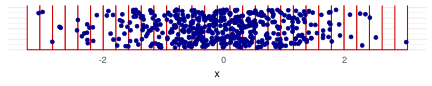
\includegraphics[width=0.7\linewidth]{Notas-Curso-Estadistica_files/figure-latex/observaciones-histograma-1} \end{center}

\begin{itemize}
\item
  Divida el número de observaciones en \(B_j\) por el tamaño de muestra \(n\) y el ancho de banda \(h\) de cada caja.
  \begin{equation*}
  f_j = \frac{n_j}{nh}
  \end{equation*}
  De esta forma si se suma las áreas definidas por el histograma da un total de 1.
\item
  Cuente la frecuencia por el tamaño de muestra \(n\) y el ancho de banda \(h\).
  \begin{equation*}
    f_j = \frac{n_j}{nh}
    \end{equation*}
\item
  Dibuje el histograma.
\end{itemize}

\begin{center}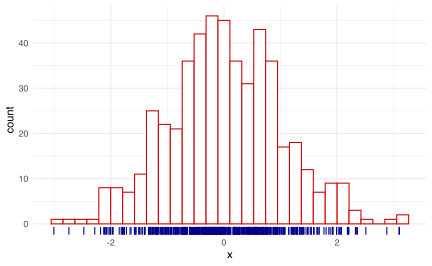
\includegraphics[width=0.7\linewidth]{Notas-Curso-Estadistica_files/figure-latex/ejemplo-inicial-histograma-1} \end{center}

Formalmente el histograma es el

\begin{equation*}
\hat{f}_h(x) = \frac{1}{nh} \sum_{i = 1}^{n} \sum_{j} I(X_i\in B_j) I(x\in B_j),
\end{equation*}

donde \(I\) es la indicadora.

\hypertarget{construcciuxf3n-probabiluxedstica}{%
\subsection{Construcción probabilística}\label{construcciuxf3n-probabiluxedstica}}

Denote \(m_j=jh-h/2\) el centro del segmento,

\begin{align*}
    \mathbb{P}\left(X\in \left[m_j - \frac{h}{2},m_j + \frac{h}{2} \right)\right)
      & =
    \int_{m_j - \frac{h}{2}}^{m_j + \frac{h}{2}} f(u)du                                             \\
      & \approx f(m_j)h
\end{align*}

Otra forma de aproximarlo es:

\begin{equation*}
    \mathbb{P} \left(X\in \left[m_j - \frac{h}{2},m_j + \frac{h}{2}\right) \right)  \approx   \frac{1}{n} \#
    \left\{X\in \left[m_j - \frac{h}{2},m_j + \frac{h}{2}\right) \right\}
\end{equation*}

Acomodando un poco la expresión

\begin{equation*}
\hat{f}_h(m_j) =  \frac{1}{nh} \#
\left\{X\in \left[m_j - \frac{h}{2},m_j + \frac{h}{2}\right) \right\}
\end{equation*}

\hypertarget{propiedades-estaduxedsticas}{%
\subsection{Propiedades estadísticas}\label{propiedades-estaduxedsticas}}

Note que el estimador de histograma \(\hat f_h\) tiende a ser más suave conforme aumenta el ancho de banda \(h\).

\hypertarget{propiedades-estaduxedsticas-1}{%
\subsection{Propiedades estadísticas}\label{propiedades-estaduxedsticas-1}}

Suponga que \(x_0 = 0\) y que \(x \in B_j\) es un punto fijo, entonces el estimador evaluado en \(x\) es:

\begin{equation*}
\hat{f}_h(x) =  \frac{1}{nh} \sum_{i = 1}^{n} I(X_i \in B_j)
\end{equation*}

\hypertarget{sesgo}{%
\subsection{Sesgo}\label{sesgo}}

Para calcular el sesgo primero calculamos:

\begin{align*}
\mathbb{E}\left[ \hat{f}_h(x)\right]
& =  \frac{1}{nh} \sum_{i = 1}^{n} \mathbb{E}\left[ I(X_i \in B_j)\right] \\
& = \frac{1}{nh} n \mathbb{E}\left[ I(X_i \in B_j)\right]
\end{align*}

donde \(I(X_i \in B_j)\) es una variable Bernoulli con valor esperado:

\begin{align*}
\mathbb{E}\left[ I(X_i \in B_j)\right] = \mathbb{P}\left(I(X_i \in
B_j)=1\right) = \int_{(j - 1)h}^{jh} f(u)du.
\end{align*}

Entonces,
\begin{align*}
\mathbb{E}\left[{f}_h(x)\right]
& = \frac{1}{h} \int_{(j - 1)h}^{jh} f(u)du
\end{align*}

y por lo tanto el sesgo de \(\hat f_h(x)\) es:
\begin{equation*}
Sesgo(\hat{f}_h(x)) = \frac{1}{h} \int_{(j -
1)h}^{jh} f(u)du - f(x)
\end{equation*}

Esto se puede aproximar usando Taylor alrededor del centro
\(m_j = jh - h/2\) de \(B_j\) de modo que
\(f(u) - f(x) \approx f^{\prime}(m_j)(u - x)\).

\begin{equation*}
Sesgo(\hat{f}_h(x)) =  \frac{1}{h} \int_{(j -
1)h}^{jh} [f(u) - f(x)] du \approx f^\prime(m_j)(m_j - x)
\end{equation*}
Entonces se puede concluir que:

\begin{itemize}
\tightlist
\item
  \(\hat f_h(x)\) es un estimador sesgado de \(f(x)\).
\item
  El sesgo tiende a ser cero cerca del punto medio de \(B_j\).
\item
  El sesgo es creciente con respecto a la pendiente de la verdadera densidad evaluada en el punto medio \(m_j\).
\end{itemize}

\hypertarget{varianza}{%
\subsection{Varianza}\label{varianza}}

Dado que todos los \(X_i\) son i.i.d., entonces

\begin{align*}
\mathrm{Var}\left( \hat{f}_h(x)\right) & =
\mathrm{Var}\left( \frac{1}{nh} \sum_{i = 1}^{n} I(X_i \in B_j)\right)                                  \\
& = \frac{1}{n^2h^2} n\mathrm{Var}\left( I(X_i \in B_j)\right)
\end{align*}

La variable \(I\) es una bernoulli con parametro
\(\int_{(j - 1)h}^{h} f(u)du\) por lo tanto su varianza es el

\begin{equation*}
\mathrm{Var}\left( \hat{f}_h(x)\right)\, =
\frac{1}{nh^2} \left(\int_{(j - 1)h}^{h} f(u)du \right)\left( 1 -\int_{(j - 1)h}^{h} f(u)du \right)
\end{equation*}

\begin{exercise}
\protect\hypertarget{exr:unnamed-chunk-4}{}\label{exr:unnamed-chunk-4}Usando un desarrollo de Taylor como en la parte anterior, pruebe que:
\begin{equation*}
\mathrm{Var}\left( \hat{f}_h(x)\right)\approx
\frac{1}{nh} f(x)
\end{equation*}
\end{exercise}

Consecuencias:

\begin{itemize}
\tightlist
\item
  La varianza del estimador es proporcional a \(f(x)\).
\item
  La varianza decrece si el ancho de banda \(h\) crece.
\end{itemize}

\hypertarget{error-cuadruxe1tico-medio}{%
\subsection{Error cuadrático medio}\label{error-cuadruxe1tico-medio}}

El error cuadrático medio del histograma es el

\begin{equation*}
\mathrm{MSE}\left( \hat{f}_h(x)\right) =
\mathrm{E}\left[\left(\hat{f}_h(x) - f(x)\right)^2\right] = \mathrm{Sesgo}^2\left( \hat{f}_h(x)\right) + \mathrm{Var}\left( \hat{f}_h(x)\right).
\end{equation*}

\begin{exercise}
\protect\hypertarget{exr:unnamed-chunk-5}{}\label{exr:unnamed-chunk-5}¿Pueden probar la segunda igualdad de la expresión anterior?
\end{exercise}

Retomando los términos anteriores se puede comprobar que:

\begin{align} 
\mathrm{MSE}\left( \hat{f}_h(x)\right) = \frac{1}{nh} f(x) +
f^\prime \left\{ \left( j - \frac{1}{2} \right) h \right\}^2 \left\{ \left( j -
\frac{1}{2} \right) h - x \right\}^2 \\
+ o\left(h \right) +        o\left(\frac{1}{nh} \right)
\label{eq:MSE}
\end{align}

\begin{remark}

Si \(h \to 0\) y \(nh \to \infty\) entonces \(\mathrm{MSE}\left( \hat{f}_h(x)\right) \to 0\). Es decir, conforme usamos más observaciones, pero el ancho de banda de banda no decrece tan rápido, entonces el error cuadrático medio converge a 0.

Como \(\mathrm{MSE}\left( \hat{f}_h(x)\right) \to 0\) (convergencia en \(\mathbb{L}^2\)) implica que \(\hat{f}_h(x) \stackrel{\mathcal{P}}{\to} f(x)\), entonces \(\hat{f}_h\) es consistente. Además según la fórmula \eqref{eq:MSE}, concluimos lo siguiente:

\begin{itemize}
\tightlist
\item
  Si \(h\to 0\), la varianza crece (converge a \(\infty\)) y el sesgo
  decrece (converge a \(f^\prime (0)x^2\)).
\item
  Si \(h\to \infty\), la varianza decrece (hacia 0) y el sesgo crece
  (hacia \(\infty\))
\end{itemize}

\end{remark}

\begin{exercise}
\protect\hypertarget{exr:unnamed-chunk-8}{}\label{exr:unnamed-chunk-8}Si \(f\sim N(0,1)\), aproxime los componentes de sesgo, varianza y MSE, y grafíquelos para distintos valores de \(h\).
\end{exercise}

Solución:

\begin{center}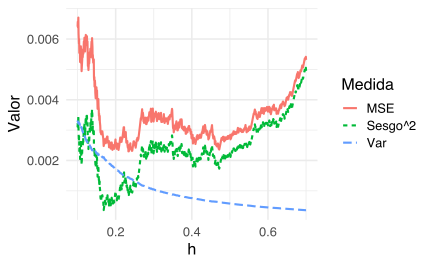
\includegraphics[width=0.7\linewidth]{Notas-Curso-Estadistica_files/figure-latex/MSE-histograma-1} \end{center}

\hypertarget{error-cuadruxe1tico-medio-integrado}{%
\subsection{Error cuadrático medio integrado}\label{error-cuadruxe1tico-medio-integrado}}

Uno de los problemas con el \(\mathrm{MSE}\left( \hat{f}_h(x)\right)\) es que depende de \(x\) y de la función de densidad \(f\) (desconocida). Integrando con respecto a \(x\) el MSE se logra resolver el primer problema:

\begin{align*}
\mathrm{MISE}\left(  \hat{f}_h\right)
& = \mathrm{E}\left[
\int_{ -\infty}^{\infty} \left\{
\hat{f}_h(x) - f(x)
\right\}^2 dx
\right]                                                       \\
& = \int_{ -\infty}^{\infty} \mathrm{E}\left[
\left\{
\hat{f}_h(x) - f(x)
\right\}^2
\right] dx                                                    \\
& = \int_{ -\infty}^{\infty}\mathrm{MSE}(\hat{f}_h(x)) \, dx
\end{align*}

Al \(\mathrm{MISE}\) se le llama error cuadrático medio integrado. Además,

\begin{align*}
\mathrm{MISE} (\hat{f}_h)
& \approx \int_{ -\infty}^{\infty} \frac{1}{nh} f(x)dx                                                                                                                                          \\
& + \int_{ -\infty}^{\infty}\, \sum_{j}^{} I(x\in B_j) \left\{ \left( j- \frac{1}{2} \right)h -x  \right\}^2 \left [f^\prime \left( \left\{j - \frac{1}{2}\right\}h \right)  \right]^2 dx \\
& = \frac{1}{nh} + \sum_{j}^{} \left [f^\prime \left( \left\{j - \frac{1}{2}\right\}h \right)  \right]^2 \int_{ B_j}    \left\{ \left( j- \frac{1}{2} \right)h -x  \right\}^2 dx          \\
& =\frac{1}{nh} + \frac{h^2}{12} \sum_{j} \left [f^\prime \left( \left\{j - \frac{1}{2}\right\}h \right)  \right]^2                                                                       \\
& \approx \frac{1}{nh} + \frac{h^2}{12} \int \{f^\prime(x)\}^2 dx                                                                                                                         \\
& =\frac{1}{nh} + \frac{h^2}{12} \Vert f^\prime\Vert_{2}^2
\end{align*}

la cual es una buena aproximación si \(h\rightarrow 0\). A este último término se le llama MISE asintótico.

\hypertarget{ancho-de-banda-uxf3ptimo-para-el-histograma}{%
\subsection{Ancho de banda óptimo para el histograma}\label{ancho-de-banda-uxf3ptimo-para-el-histograma}}

El MISE tiene un comportamiento asintótico similar al observado en el MSE. La figura siguiente presenta el comportamiento de la varianza, sesgo y MISE para nuestro ejemplo anterior:

\begin{figure}

{\centering 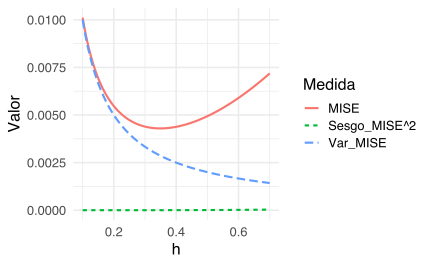
\includegraphics[width=0.7\linewidth]{Notas-Curso-Estadistica_files/figure-latex/MISE-histograma-1} 

}

\caption{ }\label{fig:MISE-histograma}
\end{figure}

Un problema frecuente en los histogramas es que la mala elección del parámetro \(h\) causa que estos no capturen toda la estructura de los datos. Por ejemplo, en el siguiente caso se muestra histogramas construídos a partir de 1000 números aleatorios según una \(N(0,1)\), bajo 4 distintas escogencias de ancho de banda.

\begin{center}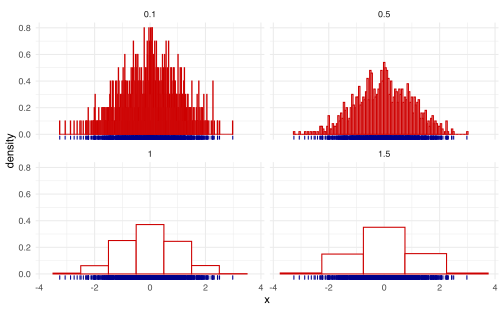
\includegraphics[width=0.7\linewidth]{Notas-Curso-Estadistica_files/figure-latex/unnamed-chunk-10-1} \end{center}

Un criterio más preciso para seleccionar el ancho de banda es a través de la minimización del MISE:

\begin{equation*}
\frac{\partial \mathrm{MISE}(f_{h})}{\partial h} = -\frac{1}{nh^2} + \frac{1}{6} h \Vert f^\prime\Vert_{2}^2 = 0
\end{equation*}

lo implica que

\begin{equation*}
h_{opt} = \left(\frac{6}{n\Vert f^\prime\Vert_{2}^2}\right) ^{1/3} = O\left( n^{-1/3} \right).
\end{equation*}

y por lo tanto

\begin{equation*}
\mathrm{MISE}(\hat{f}_{h}) = \frac{1}{n} \left(\frac{n\Vert f^\prime\Vert_{2}^2}{6}\right)  ^{1/3}
\end{equation*}

\begin{remark}[Recuerde de Estadística I]
Si \(X_1, \ldots, X_n \sim f_{\theta}\) i.i.d, con \(\mathrm{Var}(X) = \sigma^2\) y media \(\theta\), recuerde que el estimador \(\hat{\theta}\) de \(\theta\) tiene la característica que

\begin{equation*}
\mathrm{MSE}(\theta) = \mathrm{Var}(\hat{\theta}) +
\mathrm{Sesgo}^2(\hat{\theta}) = \frac{\sigma^2}{n}
\end{equation*}
\end{remark}

Según la nota anterior la tasas de convergencia del histograma es más lenta que la de un estimador parámetrico considerando la misma cantidad de datos, tal y como se ilustra en el siguiente gráfico:

\begin{center}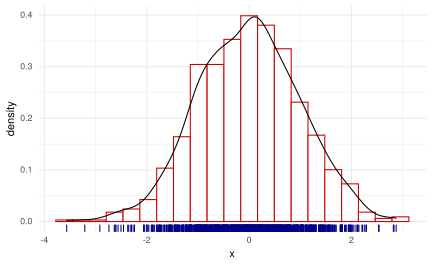
\includegraphics[width=0.7\linewidth]{Notas-Curso-Estadistica_files/figure-latex/unnamed-chunk-12-1} \end{center}

Finalmente, podemos encontrar el valor óptimo del ancho de banda (\(h=\) 0.3285) del conjunto de datos en el ejemplo anterior.

\begin{center}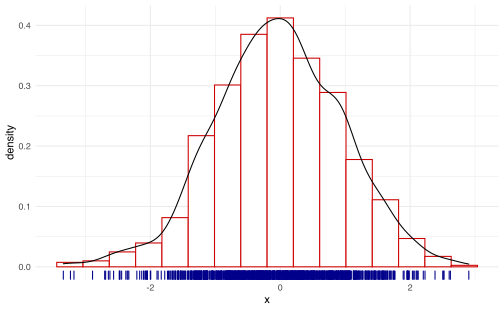
\includegraphics[width=0.7\linewidth]{Notas-Curso-Estadistica_files/figure-latex/unnamed-chunk-14-1} \end{center}

\begin{exercise}
\protect\hypertarget{exr:unnamed-chunk-15}{}\label{exr:unnamed-chunk-15}Verifique que en el caso normal estándar: \(h_{opt}\approx 3.5 n^{-1/3}\).
\end{exercise}

\hypertarget{estimaciuxf3n-de-densidades-basada-en-kernels.}{%
\section{Estimación de densidades basada en kernels.}\label{estimaciuxf3n-de-densidades-basada-en-kernels.}}

\hypertarget{primera-construcciuxf3n}{%
\subsection{Primera construcción}\label{primera-construcciuxf3n}}

Sea \(X_{1},\ldots,X_{n}\) variables aleatorias i.i.d. con distribución \(f\) en \(\mathbb{R}\). La distribución de \(f\) es \(F(x)=\int_{-\infty}^{x}f(t)dt\).

La distribución empírica de \(F\) es:
\[
F_{n}(x)=\frac{1}{n}\sum_{i=1}^{n}I(X_{i}\leq x).
\]

Por la ley de los grandes números tenemos que \(F_{n}(x) \xrightarrow{c.s} F(x)\) para todo \(x\) en \(\mathbb{R}\), conforme
\(n\rightarrow\infty\). Entonces, \(F_{n}(x)\) es un estimador consistente de \(F(x)\) para todo \(x\) in \(\mathbb{R}\).

\begin{remark}
¿Podríamos derivar \(F_n\) para encontrar el estimador \(\hat{f}_n\)?
\end{remark}

La respuesta es si (más o menos).

Suponga que \(h>0\) tenemos la aproximación
\[
f(x)\approx\frac{F(x+h)-F(x-h)}{2h}.
\]

Remplazando \(F\) por su estimador \(F_{n}\), defina
\[
\hat{f}_{n}^{R}(x)=\frac{F_{n}(x+h)-F_{n}(x-h)}{2h},
\]
donde \(\hat{f}_{n}^{R}(x)\) es el estimador de \emph{Rosenblatt} .

Podemos rescribirlo de la forma,
\[
\hat{f}_{n}^{R}(x)=\frac{1}{2nh}\sum_{i=1}^{n}I(x-h<X_{i}\leq x+h)=\frac{1}{nh}\sum_{i=1}^{n}K_{0}\left(\frac{X_{i}-x}{h}\right)
\]
con \(K_{0}(u)=\frac{1}{2}I(-1<u\leq1)\), lo cual es equivalente al caso del histograma.

\hypertarget{otra-construcciuxf3n}{%
\subsection{Otra construcción}\label{otra-construcciuxf3n}}

Con el histograma construimos una serie de segmentos fijo \(B_{j}\) y contabamos el número de datos que estaban \textbf{contenidos en \(B_{j}\)}

\begin{remark}
¿Qué pasaría si cambiamos la palabra \textbf{contenidos} por \textbf{alrededor de ``x''}?
\end{remark}

Suponga que se tienen intervalos de longitud \(2h\), es decir, intervalos de la forma \([x-h,x+h)\).

El estimador de histograma se escribe como

\begin{equation*}
\hat{f_{h}}(x) = \dfrac{1}{2hn} \# \{ X_i \in [x-h,x+h) \}.
\end{equation*}

Note que si definimos
\begin{equation*}
K(u)=\frac{1}{2} I \left( \left\vert u \right\vert \leq 1 \right)
\end{equation*}
con \(u = \frac{x-x_i}{h}\), entonces parte del estimador de histograma se puede escribir como:
\begin{equation*}
\frac{1}{2}\# \{ X_i \in [x-h,x+h) \}
=\sum_{i=1}^{n} K\left( \frac{x-x_{i}}{h} \right)
=\sum_{i=1}^{n}  \frac{1}{2} I \left( \left\vert \frac{x-x_{i}}{h}
\right\vert \leq 1 \right)
\end{equation*}

Finalmente se tendría que

\begin{equation*}
\hat{f}_{h}\left( x \right) = \frac{1}{nh}\sum_{i=1}^{n} K\left( \frac{x-x_{i}}{h} \right)
\end{equation*}

\begin{remark}
¿Qué pasaría si cambiaríamos la función \(K\) del histograma por una más general? Esto permitiría incluir la noción de ``cercanía'' de cada dato alrededor de \(x\).
\end{remark}

Esta función debería cumplir las siguientes características:

\begin{itemize}
\tightlist
\item
  \(K(u)\geq 0\).
\item
  \(\int_{-\infty}^{\infty} K(u)du = 1\).
\item
  \(\int_{-\infty}^{\infty} u K(u)du = 0\).
\item
  \(\int_{-\infty}^{\infty} u^{2} K(u)du <\infty\).
\end{itemize}

Por ejemplo:

\begin{itemize}
\tightlist
\item
  \textbf{Uniforme:} \(\frac{1}{2} I \left( \left\vert u \right\vert \leq 1 \right)\).
\item
  \textbf{Triangular:} \((1-|u|) I \left( \left\vert u \right\vert \leq 1 \right)\).
\item
  \textbf{Epanechnikov:} \(\frac{3}{4} (1-u^{2}) I \left( \left\vert u \right\vert \leq 1 \right)\).
\item
  \textbf{Gaussian:} \(\frac{1}{\sqrt{2\pi}} \exp \left( -\frac{1}{2}u^{2} \right)\).
\end{itemize}

\begin{center}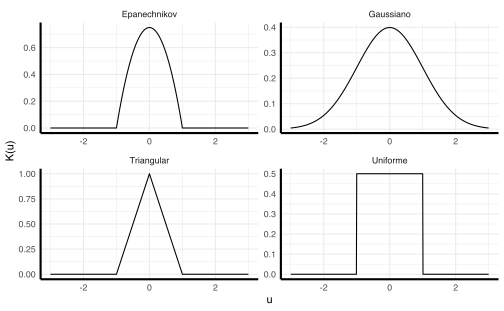
\includegraphics[width=0.7\linewidth]{Notas-Curso-Estadistica_files/figure-latex/unnamed-chunk-19-1} \end{center}

Entonces se tendría que la expresión general para un estimador por núcleos (kernel) de \(f\):

\begin{equation*}
\hat{f}_{h}\left( x \right) = \frac{1}{nh}\sum_{i=1}^{n} K\left( \frac{x-x_{i}}{h} \right)=\frac{1}{n}\sum_{i=1}^{n} K_h(x-x_{i}) 
\end{equation*}

donde \(x_1,\ldots,x_n\) es una muestra i.i.d. de \(f\),
\begin{align*}
K_h(\cdot)=\frac 1 h K(\cdot /h).
\end{align*}
y \(K\) es un kernel según las 4 propiedades anteriores.

\begin{remark}
¿Qué pasaría si modificamos el ancho de banda \(h\) para un mismo kernel?
\end{remark}

Nuevamente controlaríamos la suavidad del estimador a como se ilustra a continuación:

\begin{center}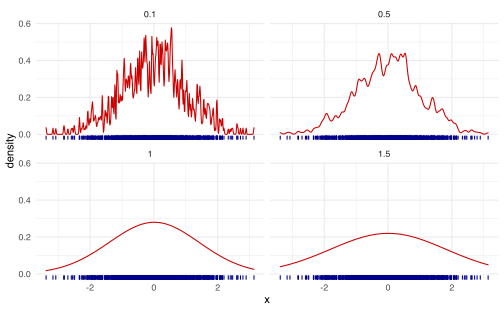
\includegraphics[width=0.7\linewidth]{Notas-Curso-Estadistica_files/figure-latex/unnamed-chunk-21-1} \end{center}

Inconveniente: no tenemos aún un criterio para un \(h\) óptimo.

\begin{remark}
¿Qué pasaría si modificamos el kernel para un mismo ancho de banda \(h\)?
\end{remark}

Usando 1000 números aleatorios según una normal estándar, con un ancho de banda fijo (\(h=0.3\)) podemos ver que no hay diferencias muy marcadas entre los estimadores por kernel:

\begin{center}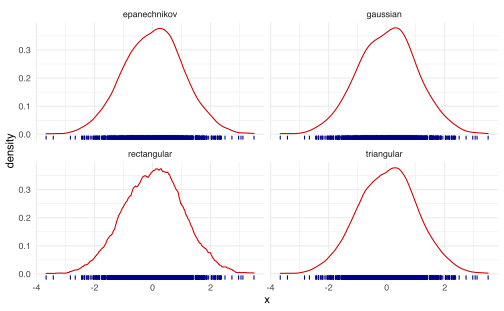
\includegraphics[width=0.7\linewidth]{Notas-Curso-Estadistica_files/figure-latex/unnamed-chunk-23-1} \end{center}

Recordemos nuevamente la fórmula

\begin{equation*}
\hat{f}_{h}\left( x \right) = \frac{1}{nh}\sum_{i=1}^{n} K\left( \frac{x-X_{i}}{h} \right)
\end{equation*}

Cada sumando de esta expresión es una función de la variable \(x\). Si la integramos se obtiene que

\begin{equation*}
\frac{1}{nh}\int K\left( \frac{x-X_{i}}{h} \right) dx
= \frac{1}{nh} \int K\left( u \right) h du
= \frac{1}{n} \int K(u) du
= \frac{1}{n}
\end{equation*}

En el siguiente gráfico se generan 10 puntos aleatorios según una normal estándar (rojo) y se grafica cada uno de los 10 componentes del estimador de la densidad usando kernels gaussianos (azul). El estimador resultante aparece en color negro. Note que cada uno de los 10 componentes tiene la misma área bajo la curva, la cual en este caso es 0.1.

\begin{center}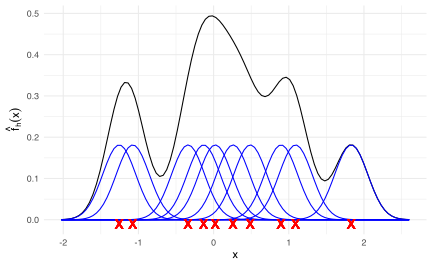
\includegraphics[width=0.7\linewidth]{Notas-Curso-Estadistica_files/figure-latex/unnamed-chunk-24-1} \end{center}

\hypertarget{propiedades-estaduxedsticas-2}{%
\subsection{Propiedades Estadísticas}\label{propiedades-estaduxedsticas-2}}

Al igual que en el caso de histograma, también aplica lo siguiente:

\begin{align*}
\mathrm{MSE}(\hat{f}_{h}(x)) & =\mathrm{Var}(\hat{f}_{h}(x))+\mathrm{Sesgo}^{2} (\hat{f}_{h}(x))            \\
\mathrm{MISE}(\hat{f}_{h})   & =\int\mathrm{Var}(\hat{f}_{h}(x))dx+\int\mathrm{Sesgo}^{2}(\hat{f}_{h}(x))dx
\end{align*}

donde

\(\mathrm{Var}\left(\hat{f}_{h}(x)\right)=\mathbb{E}\left[\hat{f}_{h}(x)-\mathbb{E}\hat{f}_{h}(x)\right]^{2}\) and \(\mathrm{Sesgo}\left(\hat{f}_{h}(x)\right)=\mathbb{E}\left[\hat{f}_{h}(x)\right]-f(x)\).

En el caso de la varianza:

\begin{align*}
\mathrm{Var}(\hat{f}_{h}(x))
& =\mathrm{Var}\left(\frac{1}{n}\sum_{i=1}^{n}K\left(\frac{x-X_{i}}{h}\right)\right)          \\
& =\frac{1}{n^{2}h^{2}}\sum_{i=1}^{n}\mathrm{Var}\left(K\left(\frac{x-X_{i}}{h}\right)\right) \\
& =\frac{1}{nh^{2}}\mathrm{Var}\left(K\left(\frac{x-X}{h}\right)\right)                       \\
& =\frac{1}{nh^{2}}\left\{
\textcolor{red}{\mathbb{E}\left[K^{2}\left(\frac{x-X}{h}\right)\right]}
-\left\{
\textcolor{blue}{\mathbb{E}\left[K\left(\frac{x-X}{h}\right)\right]}
\right\}^{2}
\right\}.
\end{align*} Usando que: \begin{align*}
\textcolor{red}{\mathbb{E}\left[K^{2}\left(\frac{x-X}{h}\right)\right]}
& =\int K^{2}\left(\frac{x-s}{h}\right)f(s)ds            \\
& =h\int K^{2}\left(u\right)f(uh+x)du                    \\
& =h\int K^{2}\left(u\right)\left\{ f(x)+o(1)\right\} du \\
& =h\left\{ \Vert K\Vert_{2}^{2}f(x)+o(1)\right\} .
\end{align*}

\begin{align*}
\textcolor{blue}{\mathbb{E}\left[K\left(\frac{x-X}{h}\right)\right]}
& =\int K\left(\frac{x-s}{h}\right)f(s)ds            \\
& = h\int K\left(u\right)f(uh+x)du                    \\
& =h\int K\left(u\right)\left\{ f(x)+o(1)\right\} du \\
& =h\left\{f(x)+o(1)\right\} .
\end{align*}

Por lo tanto se obtiene que

\begin{equation*}
\mathrm{Var}\left(\hat{f}_{h}(x)\right) = \frac{1}{nh} \Vert K\Vert_{2}^{2}f(x) + o\left(\frac{1}{nh}\right), \text{ si } nh\to \infty.
\end{equation*}

\hypertarget{sesgo-1}{%
\subsection{Sesgo}\label{sesgo-1}}

Para el sesgo tenemos

\begin{align*}
\mathrm{Sesgo}\left(\hat{f}_{h}(x)\right)
& = \mathbb{E}\left[\hat{f}_{h}(x)\right]-f(x)                                                  \\
& = \frac{1}{nh} \sum_{i=1}^{n} \mathrm{E}\left[K\left( \frac{x-X_{i}}{h} \right)\right] - f(x) \\
& = \frac{1}{h}\mathrm{E}\left[K\left( \frac{x-X_{1}}{h} \right)\right] - f(x)                  \\
& = \int \frac{1}{h} K\left( \frac{x-u}{h}\right)f(u)du -f(x)                                   \\
\end{align*}

\begin{exercise}
\protect\hypertarget{exr:unnamed-chunk-25}{}\label{exr:unnamed-chunk-25}Usando el cambio de variable \(s=\frac{u-x}{h}\) y las propiedades del kernel pruebe que

\begin{equation*}
\mathrm{Sesgo}\left(\hat{f}_{h}(x)\right) = \frac{h^{2}}{2} f^{\prime\prime} \mu_{2}(K) + o(h^{2}), \text{ si } h\to 0
\end{equation*}
donde \(\mu_{2}=\int s^{2}K(s)ds\).
\end{exercise}

\begin{remark}
En algunas pruebas más formales, se necesita además que \(f^{\prime\prime}\) sea absolutamente continua y que \(\int(f^{\prime\prime\prime}(x))dx<\infty\).\}
\end{remark}

En el siguiente gráfico se ilustra el estimador no paramétrico de la distribución de tiempos entre erupciones en la muy conocida tabla de datos \emph{faithful}. El estimador se calcula bajo dos distintas escogencias de ancho de banda.

\begin{center}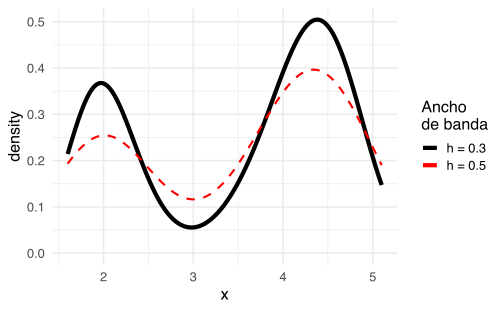
\includegraphics[width=0.7\linewidth]{Notas-Curso-Estadistica_files/figure-latex/unnamed-chunk-28-1} \end{center}

\begin{remark}
Note como los cambios en el ancho de banda modifican la suavidad (sesgo) y el aplanamiento de la curva (varianza).
\end{remark}

\hypertarget{error-cuadruxe1tico-medio-y-error-cuadruxe1tico-medio-integrado}{%
\subsection{Error cuadrático medio y Error cuadrático medio integrado}\label{error-cuadruxe1tico-medio-y-error-cuadruxe1tico-medio-integrado}}

El error cuadrático medio se escribe

\begin{align*}
\mathrm{MSE}(\hat{f}_{h}(x))
& = \mathrm{Sesgo}\left(\hat{f}_{h}(x)\right)^{2} + \mathrm{Var}\left(\hat{f}_{h}(x)\right)                                                 \\
& = \frac{h^{4}}{4}\left(\mu_{2}(K)f^{\prime\prime}(x)\right)^{2}+\frac{1}{nh}\Vert K\Vert_{2}^{2}f(x)+o(h^{4})+o\left(\frac{1}{nh}\right).
\end{align*}

Y el error cuadrático medio integrado se escribe como,

\begin{align*}
\mathrm{MISE}\left(\hat{f}_{h}\right) & = \int \mathrm{MSE}\left(\hat{f}_{h}(x)\right)dx                                                                                                        \\
& = \int \mathrm{Sesgo}\left(\hat{f}_{h}(x)\right)^{2} + \mathrm{Var}\left(\hat{f}_{h}(x)\right)dx                                                        \\
& = \frac{h^{4}}{4}\mu_{2}^{2}(K)\left\Vert f^{\prime\prime}(x)\right\Vert_{2}^{2} +\frac{1}{nh}\Vert K\Vert_{2}^{2}+o(h^{4})+o\left(\frac{1}{nh}\right).
\end{align*}

Al igual que en el caso del histograma, el estimador por kernels es un estimador consistente de \(f\) si \(h\rightarrow 0\) y \(nh\rightarrow \infty\). Además el MISE depende directamente de \(f''\).

\hypertarget{ancho-de-banda-uxf3ptimo}{%
\subsection{Ancho de banda óptimo}\label{ancho-de-banda-uxf3ptimo}}

Minimizando el \(\mathrm{MISE}\) con respecto a \(h\) obtenemos

\begin{equation*}
h_{opt}=\left(\frac{\Vert K\Vert_{2}^{2}}{\Vert f^{\prime\prime}\Vert_{2}^{2}\left(\mu_{2}(K)\right)^{2}n}\right)^{1/5}=O\left( n^{-1/5} \right).
\end{equation*}

\begin{remark}
De forma práctica, \(h_{opt}\) no es un estimador útil de \(h\) porque depende de \(\Vert f^{\prime\prime}\Vert_{2}^{2}\) que es desconocido. Más adelante veremos otra forma de encontrar este estimador.
\end{remark}

Evaluando \(h_{opt}\) en el \(\mathrm{MISE}\) tenemos que

\begin{equation*}
\mathrm{MISE}(\hat{f}_{h})=\frac{5}{4}\left(\Vert K\Vert_{2}^{2}\right)^{4/5}\left(\Vert f^{\prime\prime}\Vert_{2}^{2}\mu_{2}(K)\right)^{2/5}n^{-4/5} = O\left( n^{-4/5} \right).
\end{equation*}

y por lo tanto la tasa de convergencia del MISE a 0 es más rápida que para el caso del histograma:

\begin{center}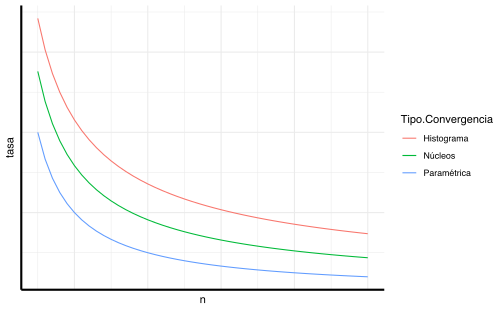
\includegraphics[width=0.7\linewidth]{Notas-Curso-Estadistica_files/figure-latex/unnamed-chunk-31-1} \end{center}

\begin{remark}
Como se comentó anteriormente, el principal inconveniente del ancho de banda:
\begin{equation*}
h_{opt}=\left(\frac{\Vert K\Vert_{2}^{2}}{\Vert f^{\prime\prime}\Vert_{2}^{2}\left(\mu_{2}(K)\right)^{2}n}\right)^{1/5}=O\left( n^{-1/5} \right).
\end{equation*}
es que depende de \(f''\).
\end{remark}

A continuación se explica dos posibles métodos para determinar para aproximar el ancho de banda óptimo:

\hypertarget{referencia-normal}{%
\subsubsection{Referencia normal}\label{referencia-normal}}

\begin{remark}
Este método es más efectivo si se conoce que la verdadera distribución es bastante suave, unimodal y simétrica. Más adelante veremos otro método para densidades más generales.
\end{remark}

Asuma que \(f\) es normal distribuida y se utiliza un kernel \(K\) gausiano.
Entonces se tiene que

\begin{align*}
\hat{h}_{rn} & =\left(\frac{\Vert K\Vert_{2}^{2}}{\Vert f^{\prime\prime}\Vert_{2}^{2}\left(\mu_{2}(K)\right)^{2}n}\right)^{1/5}=O\left( n^{-1/5} \right) \\
& =1.06 \hat{\sigma} n^{-1/5}.
\end{align*}

donde

\begin{equation*}
\hat{\sigma} = \sqrt{\frac{1}{n-1} \sum_{i=1}^{n} \left( x_{i}-\bar{x}^{2} \right)}
\end{equation*}

\begin{exercise}
\protect\hypertarget{exr:unnamed-chunk-35}{}\label{exr:unnamed-chunk-35}Pruebe que la ecuación anterior es verdadera. Utilice el hecho de que:
\begin{align*}
\Vert f^{\prime\prime}\Vert_{2}^{2}=\sigma^{-5}\int \phi^{\prime \prime}(x)^2 dx
\end{align*}
donde \(\phi\) es la función de densidad de una \(N(0,1)\).
\end{exercise}

\begin{remark}
El principal inconveniente de \(\hat{h}_{rn}\) es su sensibilidad a los valores extremos:
\end{remark}

\begin{example}
\protect\hypertarget{exm:unnamed-chunk-37}{}\label{exm:unnamed-chunk-37}La varianza empírica de 1, 2, 3, 4, 5, es 2.5.

La varianza empírica de 1, 2, 3, 4, 5, 99, es 1538.
\end{example}

Para solucionar el problema anterior, se puede considerar una medida más robusta de variación, por ejemplo el rango intercuantil IQR:

\begin{equation*}
\mathrm{IQR}^{X} = Q^{X}_{3} - Q^{X}_{1}
\end{equation*}
donde \(Q^{X}_{1}\) y \(Q^{X}_{3}\) son el primer y tercer cuartil de un conjunto de datos \(X_{1},\ldots, X_n\).

Con el supuesto que \(X\sim \mathcal{N}(\mu,\sigma^{2})\) entonces \(\displaystyle Z = \frac{X-\mu}{\sigma} \sim \mathcal{N}(0,1)\) y entonces:

\begin{align*}
\mathrm{IQR}
& = Q^{X}_{3} - Q^{X}_{1}                                                     \\
& = \left( \mu+\sigma Q^{Z}_{3} \right) - \left( \mu+\sigma Q^{Z}_{1} \right) \\
& = \sigma \left(Q^{Z}_{3} - Q^{Z}_{1} \right)                                \\
& \approx \sigma \left( 0.67 - (-0.67) \right)                                 \\
& =1.34 \sigma.
\end{align*}

Por lo tanto
\(\displaystyle \hat{\sigma} = \frac{\widehat{\mathrm{IQR}}^{X}}{1.34}\)

Podemos sustituir la varianza empírica de la fórmula inicial y tenemos
\begin{equation*}
\hat{h}_{rn} = 1.06 \frac{\widehat{\mathrm{IQR}}^{X}}{1.34} n^{-\frac{1}{5}} \approx 0.79\  \widehat{\mathrm{IQR}}^{X}\ n^{-\frac{1}{5}}
\end{equation*}

Combinando ambos estimadores, podemos obtener,

\begin{equation*}
\hat{h}_{rn} = 1.06 \min \left\{\frac{\widehat{\mathrm{IQR}}^{X}}{1.34}, \hat{\sigma }\right\} n^{-\frac{1}{5}}
\end{equation*}

pero esta aproximación es conveniente bajo el escenario de que la densidad \(f\) sea similar a una densidad normal.

\hypertarget{validaciuxf3n-cruzada}{%
\subsubsection{Validación Cruzada}\label{validaciuxf3n-cruzada}}

Defina el \emph{error cuadrático integrado} como \begin{align*}
\mathrm{ISE}(\hat{f}_{h}) & =\int\left(\hat{f}_{h}(x)-f(x)\right)^{2}dx\nonumber                   \\
& =\int \hat{f}_{h}^{2}(x)dx-2\int \hat{f}_{h}(x)f(x)dx+\int f^{2}(x)dx.
\end{align*}

\begin{remark}
El MISE es el valor esperado del ISE.
\end{remark}

Nuestro objetivo es minimizar el ISE con respecto a \(h\).

Primero note que \(\int f^{2}(x)dx\) NO DEPENDE de \(h\). Podemos minimizar
la expresión \begin{equation*}
\mathrm{ISE}(\hat{f}_{h})-\int f^{2}(x)dx=
\textcolor{red}{\int\hat{f}_{h}^{2}(x)dx}
-2
\textcolor{blue}{\int\hat{f}_{h}(x)f(x)dx}
\end{equation*}

Vamos a resolver esto en dos pasos partes

\textbf{Integral} \(\textcolor{blue}{\int\hat{f}_{h}(x)f(x)dx}\)

\textbf{Integral \(\textcolor{blue}{\int\hat{f}_{h}(x)f(x)dx}\)}

El término \(\textcolor{blue}{\int\hat{f}_{h}(x)f(x)dx}\) es el valor esperado de
\(\mathrm{E}\left[\hat{f}_h(X)\right]\). Su estimador empírico sería:
\begin{equation*}
\widehat{\mathrm{E}\left[\hat{f}_h(X)\right]}
= \frac{1}{n}\sum_{i=1}^{n}\hat{f}_{h}(X_{i})
=\frac{1}{n^{2}h}\sum_{i=1}^{n}\sum_{j=1}^{n}
K\left(\frac{X_{j}-X_{i}}{h}\right).
\end{equation*}

\begin{remark}
El problema con esta expresión es que las observaciones que se usan para estimar la esperanza son las mismas que se usan para estimar \(\hat{f}_{h}(x)\) (Se utilizan doble).
\end{remark}

La solución es remover la \(i^{\text{ésima}}\) observación de
\(\hat{f}_{h}\) para cada \(i\).

Redefiniendo el estimador anterior tenemos una estimación de \(\int \hat{f}_{h}(x)f(x)dx\) a través de:
\[
\frac{1}{n}\sum_{i=1}^{n}\hat{f}_{h,-i}(X_{i}),
\]
donde (estimador \emph{leave-one-out})
\[
\hat{f}_{h,-i}(x)=\frac{1}{(n-1)h}\sum_{\substack{j=1\\ j\neq i}}^{n}K\left( \frac{x-X_{j}}{h} \right) .
\]

de esta forma nos aseguramos que las observaciones que se usan para calcular \(\hat{f}_{h,-i}(x)\) son independientes de la observación que uno usa para definir el estimador de \(E[\hat f_h(x)]\).

Siguiendo con el término \(\textcolor{red}{\int\hat{f}_{h}^{2}(x)dx}\)
note que este se puede reescribir como

\begin{align*}
\textcolor{red}{\int\hat{f}_{h}^{2}(x)dx}
& =\int\left(\frac{1}{nh}\sum_{i=1}^{n}K\left( \frac{x-X_{i}}{h} \right)\right)^{2}dx                                    \\
& =\frac{1}{n^{2}h^{2}}\sum_{i=1}^{n}\sum_{i=1}^{n}\int K\left(\frac{x-X_{i}}{h}\right)K\left(\frac{x-X_{j}}{h}\right)dx \\
& =\frac{1}{n^{2}h}\sum_{i=1}^{n}\sum_{i=1}^{n}\int K\left(u\right)K\left(\frac{X_{i}-X_{j}}{h}-u\right)du               \\
& =\frac{1}{n^{2}h}\sum_{i=1}^{n}\sum_{i=1}^{n}K*K\left(\frac{X_{i}-X_{j}}{h}\right).
\end{align*}

donde \(K*K\) es la convolución de \(K\) consigo misma.

Finalmente tenemos la función,

Finalmente definimos la función objetivo del criterio de validación cruzada como:

\[
\mathrm{CV}(h)=\frac{1}{n^{2}h}\sum_{i=1}^{n}\sum_{j=1}^{n}K*K\left(\frac{X_{i}-X_{j}}{h}\right)-\frac{2}{n(n-1)h}\sum_{i=1}^{n}\mathop{\sum_{j=1}^{n}}_{j\neq i}K\left( \frac{X_{i}-X_{j}}{h} \right).
\]

\begin{remark}
Note que \(\mathrm{CV}(h)\) no depende de \(f\) o sus derivadas y además la función objetivo se adapta automáticamente a las características de la densidad \(f\).
\end{remark}

\hypertarget{intervalos-de-confianza-para-estimadores-de-densidad-no-paramuxe9tricos}{%
\subsection{Intervalos de confianza para estimadores de densidad no paramétricos}\label{intervalos-de-confianza-para-estimadores-de-densidad-no-paramuxe9tricos}}

Usando los resultados anteriores y asumiendo que \(h=cn^{-\frac{1}{5}}\)
entonces

\begin{equation*}
n^{\frac{2}{5}} \left\{ \hat{f}_{h}(x) -f(x)\right\}
\xrightarrow{\mathcal{L}} \mathcal{N}\left(\underbrace{\frac{c^{2}}{2} f^{\prime\prime}
\mu_{2}(K)}_{b_{x}}, \underbrace{\frac{1}{c}f(x) \left\Vert K \right\Vert_{2}^{2}}_{v_{x}}\right).
\end{equation*}

Si \(z_{1-\frac{\alpha}{2}}\) es el cuantil \(1-\frac{\alpha}{2}\) de una
distribución normal estándar, entonces

\begin{align*}
1-\alpha
& \approx \mathbb{P}\left(b_{x}-z_{1-\frac{\alpha}{2}} v_{x} \leq n^{2 / 5}\left\{\widehat{f}_{h}(x)-f(x)\right\} \leq b_{x}+z_{1-\frac{\alpha}{2}} v_{x}\right) \\
& =\mathbb{P}\left(\widehat{f}_{h}(x)-n^{-2 / 5}\left\{b_{x}+z_{1-\frac{\alpha}{2}} v_{x}\right\}\right.                                                         \\
& \qquad\qquad \left. \leq f(x)\leq \hat{f}_{h}(x)-n^{-2 / 5}\left\{b_{x}-z_{1-\frac{\alpha}{2}} v_{x}\right\}\right)
\end{align*}

Esta expresión nos dice que con una probabilidad de \(1-\alpha\) se tiene
que

\begin{equation*}
\begin{aligned}
& \left[\hat{f}_{h}(x)-\frac{h^{2}}{2} f^{\prime \prime}(x) \mu_{2}(K)-z_{1-\frac{\alpha}{2}} \sqrt{\frac{f(x)\|K\|_{2}^{2}}{n h}}\right. \\
& \left.\widehat{f}_{h}(x)-\frac{h^{2}}{2} f^{\prime \prime}(x) \mu_{2}(K)+z_{1-\frac{a}{2}} \sqrt{\frac{f(x)\|K\|_{2}^{2}}{n h}}\right]
\end{aligned}
\end{equation*}

Al igual que en los casos anteriores, este invtervalo no es útil ya que
depende de \(f(x)\) y \(f^{\prime\prime} (x)\).

Si \(h\) es pequeño relativamente a \(n^{-\frac{1}{5}}\) entonces el segundo
término \(\frac{h^{2}}{2} f^{\prime \prime}(x) \mu_{2}(K)\) podría ser
ignorado.

Si \(h\) es pequeño relativamente a \(n^{-\frac{1}{5}}\) entonces el segundo término \(\frac{h^{2}}{2} f^{\prime \prime}(x) \mu_{2}(K)\) podría ser ignorado.

Podemos reemplazar \(f(x)\) por su estimador \(\hat{f}_{h}(x)\). Entonces tendríamos una intervalo aplicable a nuestro caso:

\begin{equation*}
\left[\hat{f_{h}}(x)-z_{1-\frac{\alpha}{2}} \sqrt{\frac{\hat{f_{h}}(x)\|K\|_{2}^{2}}{n h}}, \hat{f}_{h}(x)+z_{1-\frac{\alpha}{2}} \sqrt{\frac{\hat{f}_{h}(x)\|\mathrm{K}\|_{2}^{2}}{n h}}\right]
\end{equation*}

\begin{remark}
Este intervalo de confianza está definido para \(x\) fijo y no permite hacer inferencia sobre toda la función \(f\). Una forma de determinar la banda de confianza de toda la función \(f\) es a través de la fórmula 3.52 en la página 62 de \autocite{HardleNonparametric2004}.
\end{remark}

\hypertarget{laboratorio}{%
\section{Laboratorio}\label{laboratorio}}

Comenzaremos con una librería bastante básica llamada
\texttt{KernSmooth}.

\hypertarget{efecto-de-distintos-kernels-en-la-estimaciuxf3n}{%
\subsection{Efecto de distintos Kernels en la estimación}\label{efecto-de-distintos-kernels-en-la-estimaciuxf3n}}

\begin{Shaded}
\begin{Highlighting}[]
\NormalTok{x }\OtherTok{\textless{}{-}} \FunctionTok{read.csv}\NormalTok{(}\StringTok{"data/stockres.txt"}\NormalTok{)}
\NormalTok{x }\OtherTok{\textless{}{-}} \FunctionTok{unlist}\NormalTok{(x)}
\end{Highlighting}
\end{Shaded}

\begin{Shaded}
\begin{Highlighting}[]
\FunctionTok{summary}\NormalTok{(x)}
\end{Highlighting}
\end{Shaded}

\begin{verbatim}
##       Min.    1st Qu.     Median       Mean    3rd Qu.       Max. 
## -0.6118200 -0.0204085 -0.0010632 -0.0004988  0.0215999  0.1432286
\end{verbatim}

\begin{Shaded}
\begin{Highlighting}[]
\FunctionTok{library}\NormalTok{(KernSmooth)}

\NormalTok{fhat\_normal }\OtherTok{\textless{}{-}} \FunctionTok{bkde}\NormalTok{(x, }\AttributeTok{kernel =} \StringTok{"normal"}\NormalTok{, }\AttributeTok{bandwidth =} \FloatTok{0.05}\NormalTok{)}
\FunctionTok{plot}\NormalTok{(fhat\_normal, }\AttributeTok{type =} \StringTok{"l"}\NormalTok{)}
\end{Highlighting}
\end{Shaded}

\begin{center}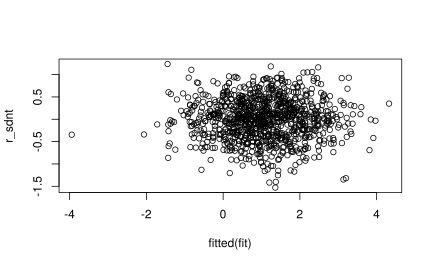
\includegraphics[width=0.7\linewidth]{Notas-Curso-Estadistica_files/figure-latex/unnamed-chunk-45-1} \end{center}

\begin{Shaded}
\begin{Highlighting}[]
\NormalTok{fhat\_unif }\OtherTok{\textless{}{-}} \FunctionTok{bkde}\NormalTok{(x, }\AttributeTok{kernel =} \StringTok{"box"}\NormalTok{, }\AttributeTok{bandwidth =} \FloatTok{0.05}\NormalTok{)}
\FunctionTok{plot}\NormalTok{(fhat\_unif, }\AttributeTok{type =} \StringTok{"l"}\NormalTok{)}
\end{Highlighting}
\end{Shaded}

\begin{center}\includegraphics[width=0.7\linewidth]{Notas-Curso-Estadistica_files/figure-latex/unnamed-chunk-45-2} \end{center}

\begin{Shaded}
\begin{Highlighting}[]
\NormalTok{fhat\_epanech }\OtherTok{\textless{}{-}} \FunctionTok{bkde}\NormalTok{(x, }\AttributeTok{kernel =} \StringTok{"epanech"}\NormalTok{, }\AttributeTok{bandwidth =} \FloatTok{0.05}\NormalTok{)}
\FunctionTok{plot}\NormalTok{(fhat\_epanech, }\AttributeTok{type =} \StringTok{"l"}\NormalTok{)}
\end{Highlighting}
\end{Shaded}

\begin{center}\includegraphics[width=0.7\linewidth]{Notas-Curso-Estadistica_files/figure-latex/unnamed-chunk-45-3} \end{center}

\begin{Shaded}
\begin{Highlighting}[]
\NormalTok{fhat\_biweight }\OtherTok{\textless{}{-}} \FunctionTok{bkde}\NormalTok{(x, }\AttributeTok{kernel =} \StringTok{"biweight"}\NormalTok{, }\AttributeTok{bandwidth =} \FloatTok{0.05}\NormalTok{)}
\FunctionTok{plot}\NormalTok{(fhat\_biweight, }\AttributeTok{type =} \StringTok{"l"}\NormalTok{)}
\end{Highlighting}
\end{Shaded}

\begin{center}\includegraphics[width=0.7\linewidth]{Notas-Curso-Estadistica_files/figure-latex/unnamed-chunk-45-4} \end{center}

\begin{Shaded}
\begin{Highlighting}[]
\NormalTok{fhat\_triweight }\OtherTok{\textless{}{-}} \FunctionTok{bkde}\NormalTok{(x, }\AttributeTok{kernel =} \StringTok{"triweight"}\NormalTok{, }\AttributeTok{bandwidth =} \FloatTok{0.05}\NormalTok{)}
\FunctionTok{plot}\NormalTok{(fhat\_triweight, }\AttributeTok{type =} \StringTok{"l"}\NormalTok{)}
\end{Highlighting}
\end{Shaded}

\begin{center}\includegraphics[width=0.7\linewidth]{Notas-Curso-Estadistica_files/figure-latex/unnamed-chunk-45-5} \end{center}

\hypertarget{efecto-del-ancho-de-banda-en-la-estimaciuxf3n}{%
\subsection{Efecto del ancho de banda en la estimación}\label{efecto-del-ancho-de-banda-en-la-estimaciuxf3n}}

** Kernel uniforme **

\begin{Shaded}
\begin{Highlighting}[]
\NormalTok{fhat }\OtherTok{\textless{}{-}} \FunctionTok{bkde}\NormalTok{(x, }\AttributeTok{kernel =} \StringTok{"box"}\NormalTok{, }\AttributeTok{bandwidth =} \FloatTok{0.001}\NormalTok{)}
\FunctionTok{plot}\NormalTok{(fhat, }\AttributeTok{type =} \StringTok{"l"}\NormalTok{)}
\end{Highlighting}
\end{Shaded}

\begin{center}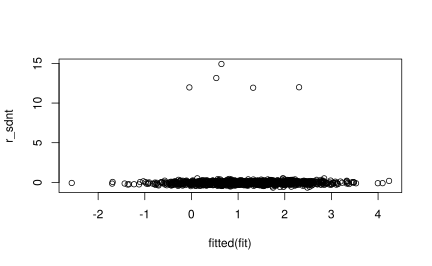
\includegraphics[width=0.7\linewidth]{Notas-Curso-Estadistica_files/figure-latex/unnamed-chunk-46-1} \end{center}

\begin{Shaded}
\begin{Highlighting}[]
\NormalTok{fhat }\OtherTok{\textless{}{-}} \FunctionTok{bkde}\NormalTok{(x, }\AttributeTok{kernel =} \StringTok{"box"}\NormalTok{, }\AttributeTok{bandwidth =} \FloatTok{0.5}\NormalTok{)}
\FunctionTok{plot}\NormalTok{(fhat, }\AttributeTok{type =} \StringTok{"l"}\NormalTok{)}
\end{Highlighting}
\end{Shaded}

\begin{center}\includegraphics[width=0.7\linewidth]{Notas-Curso-Estadistica_files/figure-latex/unnamed-chunk-46-2} \end{center}

** Kernel Epanechnikov **

\begin{Shaded}
\begin{Highlighting}[]
\NormalTok{fhat }\OtherTok{\textless{}{-}} \FunctionTok{bkde}\NormalTok{(x, }\AttributeTok{kernel =} \StringTok{"epa"}\NormalTok{, }\AttributeTok{bandwidth =} \FloatTok{0.001}\NormalTok{)}
\FunctionTok{plot}\NormalTok{(fhat, }\AttributeTok{type =} \StringTok{"l"}\NormalTok{)}
\end{Highlighting}
\end{Shaded}

\begin{center}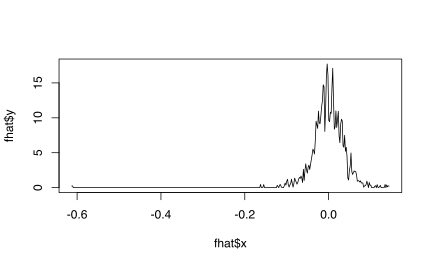
\includegraphics[width=0.7\linewidth]{Notas-Curso-Estadistica_files/figure-latex/unnamed-chunk-47-1} \end{center}

\begin{Shaded}
\begin{Highlighting}[]
\NormalTok{fhat }\OtherTok{\textless{}{-}} \FunctionTok{bkde}\NormalTok{(x, }\AttributeTok{kernel =} \StringTok{"epa"}\NormalTok{, }\AttributeTok{bandwidth =} \FloatTok{0.5}\NormalTok{)}
\FunctionTok{plot}\NormalTok{(fhat, }\AttributeTok{type =} \StringTok{"l"}\NormalTok{)}
\end{Highlighting}
\end{Shaded}

\begin{center}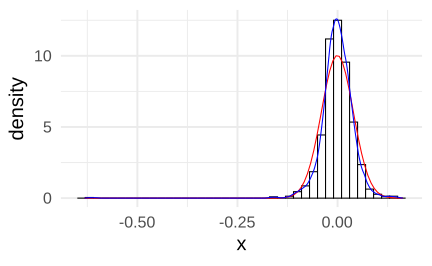
\includegraphics[width=0.7\linewidth]{Notas-Curso-Estadistica_files/figure-latex/unnamed-chunk-47-2} \end{center}

\begin{Shaded}
\begin{Highlighting}[]
\FunctionTok{suppressMessages}\NormalTok{(}\FunctionTok{library}\NormalTok{(tidyverse))}
\FunctionTok{library}\NormalTok{(gganimate)}

\NormalTok{fani }\OtherTok{\textless{}{-}} \FunctionTok{tibble}\NormalTok{()}

\ControlFlowTok{for}\NormalTok{ (b }\ControlFlowTok{in} \FunctionTok{seq}\NormalTok{(}\FloatTok{0.001}\NormalTok{, }\FloatTok{0.02}\NormalTok{, }\AttributeTok{length.out =} \DecValTok{40}\NormalTok{)) \{}
\NormalTok{    f }\OtherTok{\textless{}{-}} \FunctionTok{bkde}\NormalTok{(x, }\AttributeTok{kernel =} \StringTok{"epa"}\NormalTok{, }\AttributeTok{bandwidth =}\NormalTok{ b, }\AttributeTok{gridsize =} \FunctionTok{length}\NormalTok{(x))}
\NormalTok{    fani }\OtherTok{\textless{}{-}}\NormalTok{ fani }\SpecialCharTok{\%\textgreater{}\%}
        \FunctionTok{bind\_rows}\NormalTok{(}\FunctionTok{tibble}\NormalTok{(}\AttributeTok{xreal =} \FunctionTok{sort}\NormalTok{(x), }\AttributeTok{x =}\NormalTok{ f}\SpecialCharTok{$}\NormalTok{x,}
            \AttributeTok{y =}\NormalTok{ f}\SpecialCharTok{$}\NormalTok{y, }\AttributeTok{bw =}\NormalTok{ b))}
\NormalTok{\}}

\FunctionTok{ggplot}\NormalTok{(}\AttributeTok{data =}\NormalTok{ fani) }\SpecialCharTok{+} \FunctionTok{geom\_line}\NormalTok{(}\FunctionTok{aes}\NormalTok{(x, y), }\AttributeTok{color =} \StringTok{"blue"}\NormalTok{) }\SpecialCharTok{+}
    \FunctionTok{labs}\NormalTok{(}\AttributeTok{title =} \FunctionTok{paste0}\NormalTok{(}\StringTok{"Ancho de banda = \{closest\_state\}"}\NormalTok{)) }\SpecialCharTok{+}
    \FunctionTok{transition\_states}\NormalTok{(bw) }\SpecialCharTok{+} \FunctionTok{view\_follow}\NormalTok{() }\SpecialCharTok{+} \FunctionTok{theme\_minimal}\NormalTok{(}\AttributeTok{base\_size =} \DecValTok{20}\NormalTok{)}

\CommentTok{\# anim\_save(\textquotesingle{}manual\_figure/bandwidth{-}animation.gif\textquotesingle{})}
\end{Highlighting}
\end{Shaded}

\begin{remark}

\begin{itemize}
\tightlist
\item
  Construya una variable llamada \texttt{u} que sea una secuencia de -0.15 a 0.15 con un paso de 0.01
\item
  Asigne \texttt{x} a los datos \texttt{stockrel} y calcule su media y varianza.
\item
  Usando la función \texttt{dnorm} construya los valores de la distribución de los datos usando la media y varianza calculada anteriormente. Asigne a esta variable \texttt{f\textbackslash{}\_param}.
\item
  Defina un ancho de banda \texttt{h} en 0.02
\item
  Construya un histograma para estos datos con ancho de banda \texttt{h}. Llame a esta variable \texttt{f\textbackslash{}\_hist}
\item
  Usando el paquete \texttt{KernSmooth} y la función \texttt{bkde}, construya una función que calcule el estimador no paramétrico con un núcleo Epanechivok para un ancho de banda \(h\). Llame a esta variable \texttt{f\textbackslash{}\_epa}.
\item
  Dibuje en el mismo gráfico la estimación paramétrica y no paramétrica.
\end{itemize}

\end{remark}

\begin{Shaded}
\begin{Highlighting}[]
\NormalTok{x }\OtherTok{\textless{}{-}} \FunctionTok{read.csv}\NormalTok{(}\StringTok{"data/stockres.txt"}\NormalTok{)}
\NormalTok{x }\OtherTok{\textless{}{-}} \FunctionTok{unlist}\NormalTok{(x)}
\CommentTok{\# Eliminar nombres de las columnas}
\FunctionTok{names}\NormalTok{(x) }\OtherTok{\textless{}{-}} \ConstantTok{NULL}

\NormalTok{u }\OtherTok{\textless{}{-}} \FunctionTok{seq}\NormalTok{(}\SpecialCharTok{{-}}\FloatTok{0.15}\NormalTok{, }\FloatTok{0.15}\NormalTok{, }\AttributeTok{by =} \FloatTok{0.01}\NormalTok{)}

\NormalTok{mu }\OtherTok{\textless{}{-}} \FunctionTok{mean}\NormalTok{(x)}
\NormalTok{sigma }\OtherTok{\textless{}{-}} \FunctionTok{sd}\NormalTok{(x)}

\NormalTok{f\_param }\OtherTok{\textless{}{-}} \FunctionTok{dnorm}\NormalTok{(u, }\AttributeTok{mean =}\NormalTok{ mu, }\AttributeTok{sd =}\NormalTok{ sigma)}

\NormalTok{h }\OtherTok{\textless{}{-}} \FloatTok{0.02}

\NormalTok{n\_bins }\OtherTok{\textless{}{-}} \FunctionTok{floor}\NormalTok{(}\FunctionTok{diff}\NormalTok{(}\FunctionTok{range}\NormalTok{(x))}\SpecialCharTok{/}\NormalTok{h)}

\NormalTok{f\_hist }\OtherTok{\textless{}{-}} \FunctionTok{hist}\NormalTok{(x, }\AttributeTok{breaks =}\NormalTok{ n\_bins)}
\end{Highlighting}
\end{Shaded}

\begin{center}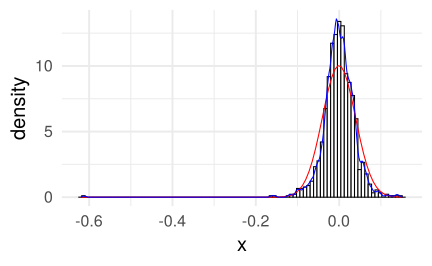
\includegraphics[width=0.7\linewidth]{Notas-Curso-Estadistica_files/figure-latex/unnamed-chunk-50-1} \end{center}

\begin{Shaded}
\begin{Highlighting}[]
\NormalTok{f\_epa }\OtherTok{\textless{}{-}} \FunctionTok{as.data.frame}\NormalTok{(}\FunctionTok{bkde}\NormalTok{(x, }\AttributeTok{kernel =} \StringTok{"epa"}\NormalTok{, }\AttributeTok{bandwidth =}\NormalTok{ h))}

\NormalTok{x\_df }\OtherTok{\textless{}{-}} \FunctionTok{data.frame}\NormalTok{(x)}

\FunctionTok{library}\NormalTok{(ggplot2)}

\FunctionTok{ggplot}\NormalTok{(x\_df, }\FunctionTok{aes}\NormalTok{(x)) }\SpecialCharTok{+} \FunctionTok{geom\_histogram}\NormalTok{(}\FunctionTok{aes}\NormalTok{(}\AttributeTok{y =}\NormalTok{ ..density..),}
    \AttributeTok{binwidth =} \FloatTok{0.02}\NormalTok{, }\AttributeTok{col =} \StringTok{"black"}\NormalTok{, }\AttributeTok{fill =} \StringTok{"white"}\NormalTok{) }\SpecialCharTok{+}
    \FunctionTok{stat\_function}\NormalTok{(}\AttributeTok{fun =}\NormalTok{ dnorm, }\AttributeTok{args =} \FunctionTok{list}\NormalTok{(}\AttributeTok{mean =}\NormalTok{ mu,}
        \AttributeTok{sd =}\NormalTok{ sigma), }\AttributeTok{color =} \StringTok{"red"}\NormalTok{) }\SpecialCharTok{+} \FunctionTok{geom\_line}\NormalTok{(}\AttributeTok{data =}\NormalTok{ f\_epa,}
    \FunctionTok{aes}\NormalTok{(x, y), }\AttributeTok{color =} \StringTok{"blue"}\NormalTok{) }\SpecialCharTok{+} \FunctionTok{theme\_minimal}\NormalTok{(}\AttributeTok{base\_size =} \DecValTok{20}\NormalTok{)}
\end{Highlighting}
\end{Shaded}

\begin{center}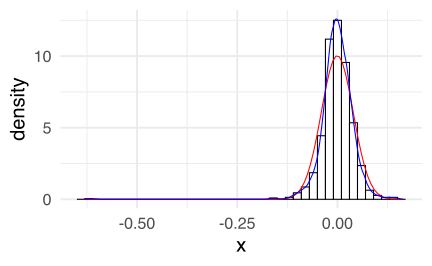
\includegraphics[width=0.7\linewidth]{Notas-Curso-Estadistica_files/figure-latex/unnamed-chunk-50-2} \end{center}

\hypertarget{ancho-de-banda-uxf3ptimo-1}{%
\subsection{Ancho de banda óptimo}\label{ancho-de-banda-uxf3ptimo-1}}

Usemos la regla de la normal o también conocida como Silverman.
\textbf{Primero recuerde que en este caso se asume que} \(f(x)\) sigue una
distribución normal. En este caso, lo que se obtiene es que

\begin{align*}
\Vert f^{\prime \prime} \Vert_2^2 & = \sigma ^{-5} \int \{\phi^{\prime \prime}\}^2 dx              \\
& = \sigma ^{-5} \frac{3}{8\sqrt{\pi}} \approx 0.212 \sigma^{-5}
\end{align*}

donde \(\phi\) es la densidad de una normal estándar.

El estimador para \(\sigma\) es

\[
s = \sqrt{\frac{1}{n-1} \sum_{i=1}^n (x_i - \bar{x})^2  }.
\]

Y usando el cálculo realizado anteriormente, se obtiene que

\[
h_{normal} = \left( \frac{4 s^5}{3n} \right)^{1/5} \approx 1.06 s n^{-1/5}.
\]

Un estimador más robusto es

\[
h_{normal} =  1.06 \min \left\{ s , \frac{IQR}{1.34} \right\} n^{-1/5}.
\]

¿Por qué es \(IQR / 1.34\)?

\begin{Shaded}
\begin{Highlighting}[]
\NormalTok{s }\OtherTok{\textless{}{-}} \FunctionTok{sd}\NormalTok{(x)}
\NormalTok{n }\OtherTok{\textless{}{-}} \FunctionTok{length}\NormalTok{(x)}
\end{Highlighting}
\end{Shaded}

\begin{Shaded}
\begin{Highlighting}[]
\NormalTok{h\_normal }\OtherTok{\textless{}{-}} \FloatTok{1.06} \SpecialCharTok{*}\NormalTok{ s }\SpecialCharTok{*}\NormalTok{ n}\SpecialCharTok{\^{}}\NormalTok{(}\SpecialCharTok{{-}}\DecValTok{1}\SpecialCharTok{/}\DecValTok{5}\NormalTok{)}

\NormalTok{h }\OtherTok{\textless{}{-}}\NormalTok{ h\_normal}

\NormalTok{n\_bins }\OtherTok{\textless{}{-}} \FunctionTok{floor}\NormalTok{(}\FunctionTok{diff}\NormalTok{(}\FunctionTok{range}\NormalTok{(x))}\SpecialCharTok{/}\NormalTok{h)}
\NormalTok{f\_hist }\OtherTok{\textless{}{-}} \FunctionTok{hist}\NormalTok{(x, }\AttributeTok{breaks =}\NormalTok{ n\_bins, }\AttributeTok{plot =} \ConstantTok{FALSE}\NormalTok{)}
\NormalTok{f\_epa }\OtherTok{\textless{}{-}} \FunctionTok{as.data.frame}\NormalTok{(}\FunctionTok{bkde}\NormalTok{(x, }\AttributeTok{kernel =} \StringTok{"epa"}\NormalTok{, }\AttributeTok{bandwidth =}\NormalTok{ h))}

\FunctionTok{ggplot}\NormalTok{(x\_df, }\FunctionTok{aes}\NormalTok{(x)) }\SpecialCharTok{+} \FunctionTok{geom\_histogram}\NormalTok{(}\FunctionTok{aes}\NormalTok{(}\AttributeTok{y =}\NormalTok{ ..density..),}
    \AttributeTok{binwidth =}\NormalTok{ h, }\AttributeTok{col =} \StringTok{"black"}\NormalTok{, }\AttributeTok{fill =} \StringTok{"white"}\NormalTok{) }\SpecialCharTok{+}
    \FunctionTok{stat\_function}\NormalTok{(}\AttributeTok{fun =}\NormalTok{ dnorm, }\AttributeTok{args =} \FunctionTok{list}\NormalTok{(}\AttributeTok{mean =}\NormalTok{ mu,}
        \AttributeTok{sd =}\NormalTok{ sigma), }\AttributeTok{color =} \StringTok{"red"}\NormalTok{) }\SpecialCharTok{+} \FunctionTok{geom\_line}\NormalTok{(}\AttributeTok{data =}\NormalTok{ f\_epa,}
    \FunctionTok{aes}\NormalTok{(x, y), }\AttributeTok{color =} \StringTok{"blue"}\NormalTok{) }\SpecialCharTok{+} \FunctionTok{theme\_minimal}\NormalTok{(}\AttributeTok{base\_size =} \DecValTok{20}\NormalTok{)}
\end{Highlighting}
\end{Shaded}

\begin{center}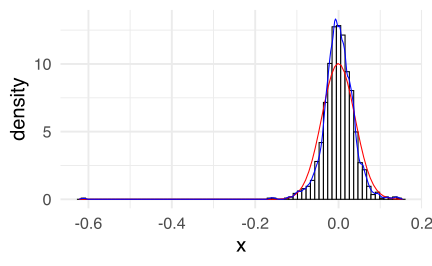
\includegraphics[width=0.7\linewidth]{Notas-Curso-Estadistica_files/figure-latex/unnamed-chunk-52-1} \end{center}

\begin{Shaded}
\begin{Highlighting}[]
\NormalTok{h\_iqr }\OtherTok{\textless{}{-}} \FloatTok{1.06} \SpecialCharTok{*} \FunctionTok{min}\NormalTok{(s, }\FunctionTok{IQR}\NormalTok{(x)}\SpecialCharTok{/}\FloatTok{1.34}\NormalTok{) }\SpecialCharTok{*}\NormalTok{ n}\SpecialCharTok{\^{}}\NormalTok{(}\SpecialCharTok{{-}}\DecValTok{1}\SpecialCharTok{/}\DecValTok{5}\NormalTok{)}

\NormalTok{h }\OtherTok{\textless{}{-}}\NormalTok{ h\_iqr}

\NormalTok{n\_bins }\OtherTok{\textless{}{-}} \FunctionTok{floor}\NormalTok{(}\FunctionTok{diff}\NormalTok{(}\FunctionTok{range}\NormalTok{(x))}\SpecialCharTok{/}\NormalTok{h)}
\NormalTok{f\_hist }\OtherTok{\textless{}{-}} \FunctionTok{hist}\NormalTok{(x, }\AttributeTok{breaks =}\NormalTok{ n\_bins, }\AttributeTok{plot =} \ConstantTok{FALSE}\NormalTok{)}
\NormalTok{f\_epa }\OtherTok{\textless{}{-}} \FunctionTok{as.data.frame}\NormalTok{(}\FunctionTok{bkde}\NormalTok{(x, }\AttributeTok{kernel =} \StringTok{"epa"}\NormalTok{, }\AttributeTok{bandwidth =}\NormalTok{ h))}

\FunctionTok{ggplot}\NormalTok{(x\_df, }\FunctionTok{aes}\NormalTok{(x)) }\SpecialCharTok{+} \FunctionTok{geom\_histogram}\NormalTok{(}\FunctionTok{aes}\NormalTok{(}\AttributeTok{y =}\NormalTok{ ..density..),}
    \AttributeTok{binwidth =}\NormalTok{ h, }\AttributeTok{col =} \StringTok{"black"}\NormalTok{, }\AttributeTok{fill =} \StringTok{"white"}\NormalTok{) }\SpecialCharTok{+}
    \FunctionTok{stat\_function}\NormalTok{(}\AttributeTok{fun =}\NormalTok{ dnorm, }\AttributeTok{args =} \FunctionTok{list}\NormalTok{(}\AttributeTok{mean =}\NormalTok{ mu,}
        \AttributeTok{sd =}\NormalTok{ sigma), }\AttributeTok{color =} \StringTok{"red"}\NormalTok{) }\SpecialCharTok{+} \FunctionTok{geom\_line}\NormalTok{(}\AttributeTok{data =}\NormalTok{ f\_epa,}
    \FunctionTok{aes}\NormalTok{(x, y), }\AttributeTok{color =} \StringTok{"blue"}\NormalTok{) }\SpecialCharTok{+} \FunctionTok{theme\_minimal}\NormalTok{(}\AttributeTok{base\_size =} \DecValTok{20}\NormalTok{)}
\end{Highlighting}
\end{Shaded}

\begin{center}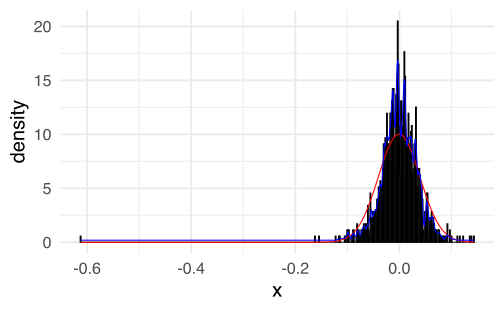
\includegraphics[width=0.7\linewidth]{Notas-Curso-Estadistica_files/figure-latex/unnamed-chunk-53-1} \end{center}

Una librería más especializada es \texttt{np} (non-parametric).

\begin{Shaded}
\begin{Highlighting}[]
\FunctionTok{library}\NormalTok{(np)}

\NormalTok{x.eval }\OtherTok{\textless{}{-}} \FunctionTok{seq}\NormalTok{(}\SpecialCharTok{{-}}\FloatTok{0.2}\NormalTok{, }\FloatTok{0.2}\NormalTok{, }\AttributeTok{length.out =} \DecValTok{200}\NormalTok{)}

\NormalTok{h\_normal\_np }\OtherTok{\textless{}{-}} \FunctionTok{npudensbw}\NormalTok{(}\AttributeTok{dat =}\NormalTok{ x, }\AttributeTok{bwmethod =} \StringTok{"normal{-}reference"}\NormalTok{)}

\NormalTok{dens.ksum }\OtherTok{\textless{}{-}} \FunctionTok{npksum}\NormalTok{(}\AttributeTok{txdat =}\NormalTok{ x, }\AttributeTok{exdat =}\NormalTok{ x.eval, }\AttributeTok{bws =}\NormalTok{ h\_normal\_np}\SpecialCharTok{$}\NormalTok{bw)}\SpecialCharTok{$}\NormalTok{ksum}\SpecialCharTok{/}\NormalTok{(n }\SpecialCharTok{*}
\NormalTok{    h\_normal\_np}\SpecialCharTok{$}\NormalTok{bw[}\DecValTok{1}\NormalTok{])}

\NormalTok{dens.ksum.df }\OtherTok{\textless{}{-}} \FunctionTok{data.frame}\NormalTok{(}\AttributeTok{x =}\NormalTok{ x.eval, }\AttributeTok{y =}\NormalTok{ dens.ksum)}

\FunctionTok{ggplot}\NormalTok{(x\_df, }\FunctionTok{aes}\NormalTok{(x)) }\SpecialCharTok{+} \FunctionTok{geom\_histogram}\NormalTok{(}\FunctionTok{aes}\NormalTok{(}\AttributeTok{y =}\NormalTok{ ..density..),}
    \AttributeTok{binwidth =}\NormalTok{ h\_normal\_np}\SpecialCharTok{$}\NormalTok{bw, }\AttributeTok{col =} \StringTok{"black"}\NormalTok{, }\AttributeTok{fill =} \StringTok{"white"}\NormalTok{) }\SpecialCharTok{+}
    \FunctionTok{stat\_function}\NormalTok{(}\AttributeTok{fun =}\NormalTok{ dnorm, }\AttributeTok{args =} \FunctionTok{list}\NormalTok{(}\AttributeTok{mean =}\NormalTok{ mu,}
        \AttributeTok{sd =}\NormalTok{ sigma), }\AttributeTok{color =} \StringTok{"red"}\NormalTok{) }\SpecialCharTok{+} \FunctionTok{geom\_line}\NormalTok{(}\AttributeTok{data =}\NormalTok{ dens.ksum.df,}
    \FunctionTok{aes}\NormalTok{(x, y), }\AttributeTok{color =} \StringTok{"blue"}\NormalTok{) }\SpecialCharTok{+} \FunctionTok{theme\_minimal}\NormalTok{(}\AttributeTok{base\_size =} \DecValTok{20}\NormalTok{)}
\end{Highlighting}
\end{Shaded}

\begin{center}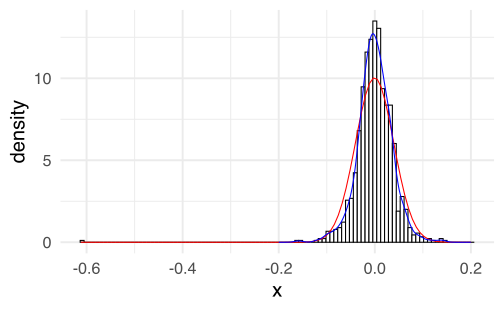
\includegraphics[width=0.7\linewidth]{Notas-Curso-Estadistica_files/figure-latex/unnamed-chunk-54-1} \end{center}

\hypertarget{validaciuxf3n-cruzada-1}{%
\subsection{Validación cruzada}\label{validaciuxf3n-cruzada-1}}

La forma que vimos en clase es la de validación cruzada por mínimos
cuadrados``least-square cross validation'\,' la cual se puede ejecutar
con este comando.

\begin{Shaded}
\begin{Highlighting}[]
\NormalTok{h\_cv\_np\_ls }\OtherTok{\textless{}{-}} \FunctionTok{npudensbw}\NormalTok{(}\AttributeTok{dat =}\NormalTok{ x, }\AttributeTok{bwmethod =} \StringTok{"cv.ls"}\NormalTok{,}
    \AttributeTok{ckertype =} \StringTok{"epa"}\NormalTok{, }\AttributeTok{ckerorder =} \DecValTok{2}\NormalTok{)}
\end{Highlighting}
\end{Shaded}

\begin{verbatim}
## Multistart 1 of 1 |Multistart 1 of 1 |Multistart 1 of 1 |Multistart 1 of 1 /Multistart 1 of 1 |Multistart 1 of 1 |                   
\end{verbatim}

\begin{Shaded}
\begin{Highlighting}[]
\NormalTok{dens.np }\OtherTok{\textless{}{-}} \FunctionTok{npudens}\NormalTok{(h\_cv\_np\_ls)}

\FunctionTok{plot}\NormalTok{(dens.np, }\AttributeTok{type =} \StringTok{"b"}\NormalTok{)}
\end{Highlighting}
\end{Shaded}

\begin{center}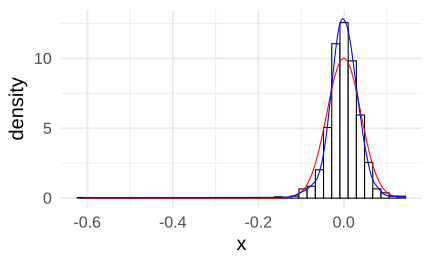
\includegraphics[width=0.7\linewidth]{Notas-Curso-Estadistica_files/figure-latex/unnamed-chunk-55-1} \end{center}

\begin{Shaded}
\begin{Highlighting}[]
\NormalTok{dens.np.df }\OtherTok{\textless{}{-}} \FunctionTok{data.frame}\NormalTok{(}\AttributeTok{x =}\NormalTok{ dens.np}\SpecialCharTok{$}\NormalTok{eval[, }\DecValTok{1}\NormalTok{], }\AttributeTok{y =}\NormalTok{ dens.np}\SpecialCharTok{$}\NormalTok{dens)}

\FunctionTok{ggplot}\NormalTok{(x\_df, }\FunctionTok{aes}\NormalTok{(x)) }\SpecialCharTok{+} \FunctionTok{geom\_histogram}\NormalTok{(}\FunctionTok{aes}\NormalTok{(}\AttributeTok{y =}\NormalTok{ ..density..),}
    \AttributeTok{binwidth =}\NormalTok{ h\_cv\_np\_ls}\SpecialCharTok{$}\NormalTok{bw, }\AttributeTok{col =} \StringTok{"black"}\NormalTok{, }\AttributeTok{fill =} \StringTok{"white"}\NormalTok{) }\SpecialCharTok{+}
    \FunctionTok{stat\_function}\NormalTok{(}\AttributeTok{fun =}\NormalTok{ dnorm, }\AttributeTok{args =} \FunctionTok{list}\NormalTok{(}\AttributeTok{mean =}\NormalTok{ mu,}
        \AttributeTok{sd =}\NormalTok{ sigma), }\AttributeTok{color =} \StringTok{"red"}\NormalTok{) }\SpecialCharTok{+} \FunctionTok{geom\_line}\NormalTok{(}\AttributeTok{data =}\NormalTok{ dens.np.df,}
    \FunctionTok{aes}\NormalTok{(x, y), }\AttributeTok{color =} \StringTok{"blue"}\NormalTok{) }\SpecialCharTok{+} \FunctionTok{theme\_minimal}\NormalTok{(}\AttributeTok{base\_size =} \DecValTok{20}\NormalTok{)}
\end{Highlighting}
\end{Shaded}

\begin{center}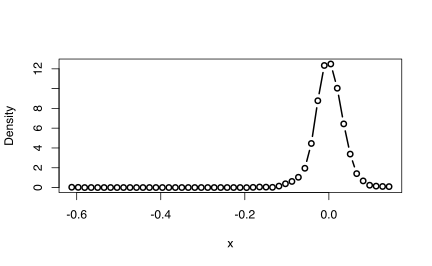
\includegraphics[width=0.7\linewidth]{Notas-Curso-Estadistica_files/figure-latex/unnamed-chunk-56-1} \end{center}

\hypertarget{temas-adicionales}{%
\subsection{Temas adicionales}\label{temas-adicionales}}

** Reducción del sesgo ** Como lo mencionamos en el texto, una forma
de mejorar el sesgo en la estimación es suponer que la función de
densidad es más veces diferenciable.

Esto se logra asumiendo que el Kernel es más veces diferenciable.

\begin{Shaded}
\begin{Highlighting}[]
\NormalTok{h\_cv\_np\_ls }\OtherTok{\textless{}{-}} \FunctionTok{npudensbw}\NormalTok{(}\AttributeTok{dat =}\NormalTok{ x, }\AttributeTok{bwmethod =} \StringTok{"cv.ls"}\NormalTok{,}
    \AttributeTok{ckertype =} \StringTok{"epa"}\NormalTok{, }\AttributeTok{ckerorder =} \DecValTok{4}\NormalTok{)}
\end{Highlighting}
\end{Shaded}

\begin{verbatim}
## Multistart 1 of 1 |Multistart 1 of 1 |Multistart 1 of 1 |Multistart 1 of 1 /Multistart 1 of 1 |Multistart 1 of 1 |                   
\end{verbatim}

\begin{Shaded}
\begin{Highlighting}[]
\NormalTok{dens.np }\OtherTok{\textless{}{-}} \FunctionTok{npudens}\NormalTok{(h\_cv\_np\_ls)}

\FunctionTok{plot}\NormalTok{(dens.np, }\AttributeTok{type =} \StringTok{"b"}\NormalTok{, }\AttributeTok{lwd =} \DecValTok{2}\NormalTok{)}
\end{Highlighting}
\end{Shaded}

\begin{center}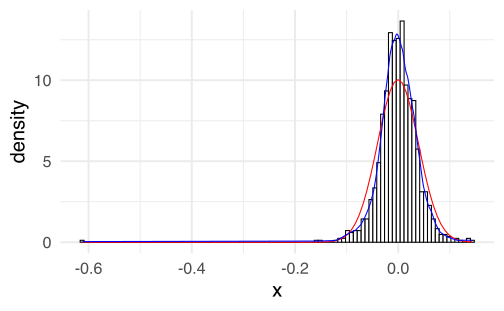
\includegraphics[width=0.7\linewidth]{Notas-Curso-Estadistica_files/figure-latex/unnamed-chunk-57-1} \end{center}

\begin{Shaded}
\begin{Highlighting}[]
\NormalTok{dens.np.df }\OtherTok{\textless{}{-}} \FunctionTok{data.frame}\NormalTok{(}\AttributeTok{x =}\NormalTok{ dens.np}\SpecialCharTok{$}\NormalTok{eval[, }\DecValTok{1}\NormalTok{], }\AttributeTok{y =}\NormalTok{ dens.np}\SpecialCharTok{$}\NormalTok{dens)}

\FunctionTok{ggplot}\NormalTok{(x\_df, }\FunctionTok{aes}\NormalTok{(x)) }\SpecialCharTok{+} \FunctionTok{geom\_histogram}\NormalTok{(}\FunctionTok{aes}\NormalTok{(}\AttributeTok{y =}\NormalTok{ ..density..),}
    \AttributeTok{binwidth =}\NormalTok{ h\_cv\_np\_ls}\SpecialCharTok{$}\NormalTok{bw, }\AttributeTok{col =} \StringTok{"black"}\NormalTok{, }\AttributeTok{fill =} \StringTok{"white"}\NormalTok{) }\SpecialCharTok{+}
    \FunctionTok{stat\_function}\NormalTok{(}\AttributeTok{fun =}\NormalTok{ dnorm, }\AttributeTok{args =} \FunctionTok{list}\NormalTok{(}\AttributeTok{mean =}\NormalTok{ mu,}
        \AttributeTok{sd =}\NormalTok{ sigma), }\AttributeTok{color =} \StringTok{"red"}\NormalTok{) }\SpecialCharTok{+} \FunctionTok{geom\_line}\NormalTok{(}\AttributeTok{data =}\NormalTok{ dens.np.df,}
    \FunctionTok{aes}\NormalTok{(x, y), }\AttributeTok{color =} \StringTok{"blue"}\NormalTok{) }\SpecialCharTok{+} \FunctionTok{theme\_minimal}\NormalTok{(}\AttributeTok{base\_size =} \DecValTok{20}\NormalTok{)}
\end{Highlighting}
\end{Shaded}

\begin{center}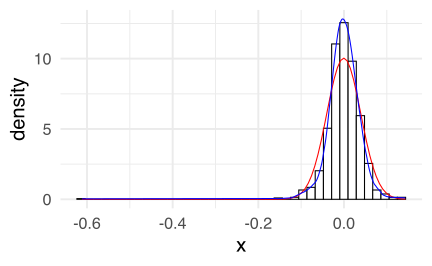
\includegraphics[width=0.7\linewidth]{Notas-Curso-Estadistica_files/figure-latex/unnamed-chunk-58-1} \end{center}

\textbf{Otra forma de estimar el ancho de banda} Otra forma de estimar ancho
de bandas óptimos es usando máxima verosimilitud. Les dejo de tarea
revisar la sección 1.1 del artículo de \autocite{Hall1987} para entender su
estructura.

\begin{Shaded}
\begin{Highlighting}[]
\NormalTok{h\_cv\_np\_ml }\OtherTok{\textless{}{-}} \FunctionTok{npudensbw}\NormalTok{(}\AttributeTok{dat =}\NormalTok{ x, }\AttributeTok{bwmethod =} \StringTok{"cv.ml"}\NormalTok{,}
    \AttributeTok{ckertype =} \StringTok{"epanechnikov"}\NormalTok{)}
\end{Highlighting}
\end{Shaded}

\begin{verbatim}
## Multistart 1 of 1 |Multistart 1 of 1 |Multistart 1 of 1 |Multistart 1 of 1 /Multistart 1 of 1 |Multistart 1 of 1 |                   
\end{verbatim}

\begin{Shaded}
\begin{Highlighting}[]
\NormalTok{dens.np }\OtherTok{\textless{}{-}} \FunctionTok{npudens}\NormalTok{(h\_cv\_np\_ml)}

\FunctionTok{plot}\NormalTok{(dens.np, }\AttributeTok{type =} \StringTok{"b"}\NormalTok{)}
\end{Highlighting}
\end{Shaded}

\begin{center}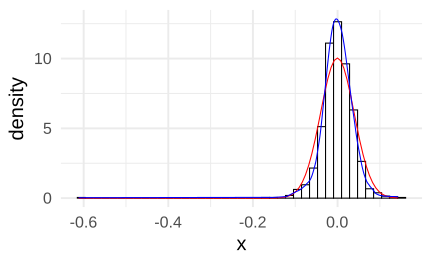
\includegraphics[width=0.7\linewidth]{Notas-Curso-Estadistica_files/figure-latex/unnamed-chunk-59-1} \end{center}

\begin{Shaded}
\begin{Highlighting}[]
\NormalTok{dens.np.df }\OtherTok{\textless{}{-}} \FunctionTok{data.frame}\NormalTok{(}\AttributeTok{x =}\NormalTok{ dens.np}\SpecialCharTok{$}\NormalTok{eval[, }\DecValTok{1}\NormalTok{], }\AttributeTok{y =}\NormalTok{ dens.np}\SpecialCharTok{$}\NormalTok{dens)}

\FunctionTok{ggplot}\NormalTok{(x\_df, }\FunctionTok{aes}\NormalTok{(x)) }\SpecialCharTok{+} \FunctionTok{geom\_histogram}\NormalTok{(}\FunctionTok{aes}\NormalTok{(}\AttributeTok{y =}\NormalTok{ ..density..),}
    \AttributeTok{binwidth =}\NormalTok{ h\_cv\_np\_ml}\SpecialCharTok{$}\NormalTok{bw, }\AttributeTok{col =} \StringTok{"black"}\NormalTok{, }\AttributeTok{fill =} \StringTok{"white"}\NormalTok{) }\SpecialCharTok{+}
    \FunctionTok{stat\_function}\NormalTok{(}\AttributeTok{fun =}\NormalTok{ dnorm, }\AttributeTok{args =} \FunctionTok{list}\NormalTok{(}\AttributeTok{mean =}\NormalTok{ mu,}
        \AttributeTok{sd =}\NormalTok{ sigma), }\AttributeTok{color =} \StringTok{"red"}\NormalTok{) }\SpecialCharTok{+} \FunctionTok{geom\_line}\NormalTok{(}\AttributeTok{data =}\NormalTok{ dens.np.df,}
    \FunctionTok{aes}\NormalTok{(x, y), }\AttributeTok{color =} \StringTok{"blue"}\NormalTok{) }\SpecialCharTok{+} \FunctionTok{theme\_minimal}\NormalTok{(}\AttributeTok{base\_size =} \DecValTok{20}\NormalTok{)}
\end{Highlighting}
\end{Shaded}

\begin{center}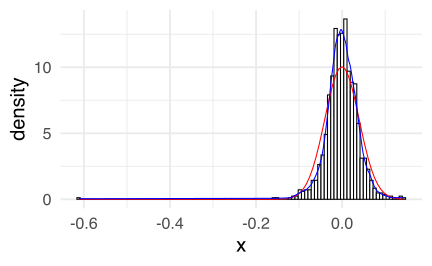
\includegraphics[width=0.7\linewidth]{Notas-Curso-Estadistica_files/figure-latex/unnamed-chunk-60-1} \end{center}

\begin{Shaded}
\begin{Highlighting}[]
\NormalTok{h\_cv\_np\_ml }\OtherTok{\textless{}{-}} \FunctionTok{npudensbw}\NormalTok{(}\AttributeTok{dat =}\NormalTok{ x, }\AttributeTok{bwmethod =} \StringTok{"cv.ml"}\NormalTok{,}
    \AttributeTok{ckertype =} \StringTok{"epanechnikov"}\NormalTok{, }\AttributeTok{ckerorder =} \DecValTok{4}\NormalTok{)}
\end{Highlighting}
\end{Shaded}

\begin{verbatim}
## Multistart 1 of 1 |Multistart 1 of 1 |Multistart 1 of 1 |Multistart 1 of 1 /Multistart 1 of 1 |Multistart 1 of 1 |                   
\end{verbatim}

\begin{Shaded}
\begin{Highlighting}[]
\NormalTok{dens.np }\OtherTok{\textless{}{-}} \FunctionTok{npudens}\NormalTok{(h\_cv\_np\_ml)}

\FunctionTok{plot}\NormalTok{(dens.np, }\AttributeTok{type =} \StringTok{"b"}\NormalTok{)}
\end{Highlighting}
\end{Shaded}

\begin{center}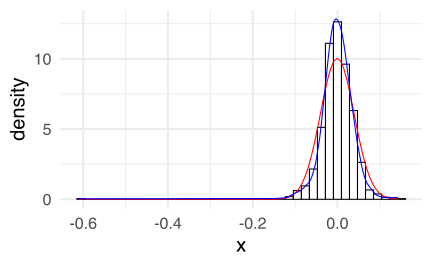
\includegraphics[width=0.7\linewidth]{Notas-Curso-Estadistica_files/figure-latex/unnamed-chunk-61-1} \end{center}

\begin{Shaded}
\begin{Highlighting}[]
\NormalTok{dens.np.df }\OtherTok{\textless{}{-}} \FunctionTok{data.frame}\NormalTok{(}\AttributeTok{x =}\NormalTok{ dens.np}\SpecialCharTok{$}\NormalTok{eval[, }\DecValTok{1}\NormalTok{], }\AttributeTok{y =}\NormalTok{ dens.np}\SpecialCharTok{$}\NormalTok{dens)}

\FunctionTok{ggplot}\NormalTok{(x\_df, }\FunctionTok{aes}\NormalTok{(x)) }\SpecialCharTok{+} \FunctionTok{geom\_histogram}\NormalTok{(}\FunctionTok{aes}\NormalTok{(}\AttributeTok{y =}\NormalTok{ ..density..),}
    \AttributeTok{binwidth =}\NormalTok{ h\_cv\_np\_ml}\SpecialCharTok{$}\NormalTok{bw, }\AttributeTok{col =} \StringTok{"black"}\NormalTok{, }\AttributeTok{fill =} \StringTok{"white"}\NormalTok{) }\SpecialCharTok{+}
    \FunctionTok{stat\_function}\NormalTok{(}\AttributeTok{fun =}\NormalTok{ dnorm, }\AttributeTok{args =} \FunctionTok{list}\NormalTok{(}\AttributeTok{mean =}\NormalTok{ mu,}
        \AttributeTok{sd =}\NormalTok{ sigma), }\AttributeTok{color =} \StringTok{"red"}\NormalTok{) }\SpecialCharTok{+} \FunctionTok{geom\_line}\NormalTok{(}\AttributeTok{data =}\NormalTok{ dens.np.df,}
    \FunctionTok{aes}\NormalTok{(x, y), }\AttributeTok{color =} \StringTok{"blue"}\NormalTok{) }\SpecialCharTok{+} \FunctionTok{theme\_minimal}\NormalTok{(}\AttributeTok{base\_size =} \DecValTok{20}\NormalTok{)}
\end{Highlighting}
\end{Shaded}

\begin{center}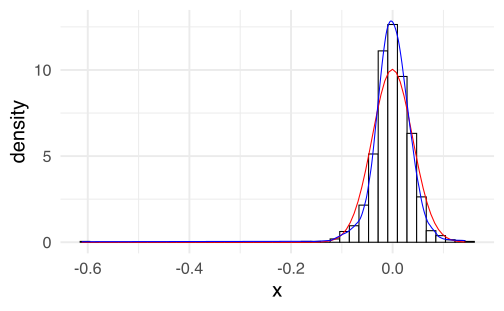
\includegraphics[width=0.7\linewidth]{Notas-Curso-Estadistica_files/figure-latex/unnamed-chunk-62-1} \end{center}

\begin{Shaded}
\begin{Highlighting}[]
\NormalTok{fani }\OtherTok{\textless{}{-}} \FunctionTok{tibble}\NormalTok{()}

\ControlFlowTok{for}\NormalTok{ (b }\ControlFlowTok{in} \FunctionTok{seq}\NormalTok{(}\FloatTok{0.001}\NormalTok{, }\FloatTok{0.05}\NormalTok{, }\AttributeTok{length.out =} \DecValTok{40}\NormalTok{)) \{}
\NormalTok{    f }\OtherTok{\textless{}{-}} \FunctionTok{npudens}\NormalTok{(}\AttributeTok{tdat =}\NormalTok{ x, }\AttributeTok{ckertype =} \StringTok{"epanechnikov"}\NormalTok{,}
        \AttributeTok{bandwidth.compute =} \ConstantTok{FALSE}\NormalTok{, }\AttributeTok{bws =}\NormalTok{ b)}
\NormalTok{    fani }\OtherTok{\textless{}{-}}\NormalTok{ fani }\SpecialCharTok{\%\textgreater{}\%}
        \FunctionTok{bind\_rows}\NormalTok{(}\FunctionTok{tibble}\NormalTok{(}\AttributeTok{xreal =} \FunctionTok{sort}\NormalTok{(x), }\AttributeTok{x =}\NormalTok{ f}\SpecialCharTok{$}\NormalTok{eval}\SpecialCharTok{$}\NormalTok{x,}
            \AttributeTok{y =}\NormalTok{ f}\SpecialCharTok{$}\NormalTok{dens, }\AttributeTok{bw =}\NormalTok{ b))}
\NormalTok{\}}

\FunctionTok{ggplot}\NormalTok{(}\AttributeTok{data =}\NormalTok{ fani) }\SpecialCharTok{+} \FunctionTok{geom\_line}\NormalTok{(}\FunctionTok{aes}\NormalTok{(x, y), }\AttributeTok{color =} \StringTok{"blue"}\NormalTok{) }\SpecialCharTok{+}
    \FunctionTok{labs}\NormalTok{(}\AttributeTok{title =} \FunctionTok{paste0}\NormalTok{(}\StringTok{"Ancho de banda = \{closest\_state\}"}\NormalTok{)) }\SpecialCharTok{+}
    \FunctionTok{theme\_minimal}\NormalTok{(}\AttributeTok{base\_size =} \DecValTok{20}\NormalTok{) }\SpecialCharTok{+} \FunctionTok{transition\_states}\NormalTok{(bw) }\SpecialCharTok{+}
    \FunctionTok{view\_follow}\NormalTok{()}

\CommentTok{\# anim\_save(\textquotesingle{}manual\_figure/bandwidth{-}animation{-}np.gif\textquotesingle{})}
\end{Highlighting}
\end{Shaded}

\begin{exercise}
\protect\hypertarget{exr:unnamed-chunk-64}{}\label{exr:unnamed-chunk-64}Implementar el intervalo confianza visto en clase para estimadores de densidades por núcleos y visualizarlo de en ggplot.

\textbf{Si se atreven: ¿Se podría hacer una versión animada de ese gráfico para visualizar el significado real de este el intervalo de confianza?}
\end{exercise}

\hypertarget{ejercicios}{%
\section{Ejercicios}\label{ejercicios}}

Del libro de \autocite{HardleNonparametric2004} hagan los siguientes ejercicios

\begin{enumerate}
\def\labelenumi{\arabic{enumi}.}
\tightlist
\item
  \textbf{Sección 2:} 1, 2, 3, 5, 7, 14
\item
  \textbf{Sección 3:} 4, 8, 10, 11, 16,
\end{enumerate}

\hypertarget{jackknife-y-bootstrap}{%
\chapter{Jackknife y Bootstrap}\label{jackknife-y-bootstrap}}

Suponga que se quiere estimar un intervalo de confianza para la media
\(\mu\) desconocida de un conjunto de datos \(X_{1},\ldots, X_{n}\)
que tiene distribución \(\mathcal{N}\left(\mu ,\sigma^{2}\right)\).

Primero se conoce que

\begin{equation*}
\sqrt{n}\left( \hat{\mu} - \mu \right)
\sim \mathcal{N}\left(0,\sigma^{2}\right),
\end{equation*}

y esto nos permite escribir el intervalo de confianza como

\begin{equation*}
\left[ \hat{\mu} - \hat{\sigma}z_{1-\frac{\alpha}{2}} ,
\hat{\mu} + \hat{\sigma}z_{1-\frac{\alpha}{2}}\right]
\end{equation*}

donde \(z_{1-\frac{\alpha}{2}}\) es el cuantil \(1-\frac{\alpha}{2}\)
de una normal estándar.

La expresión anterior es posible dado que la distribución de \(\hat{\mu}\) es normal.

\begin{remark}
¿Qué pasaría si no conocemos la distribución de \(\hat{\mu}\)?

¿Cómo podemos encontrar ese intervalo de confianza?
\end{remark}

\hypertarget{caso-concreto}{%
\section{Caso concreto}\label{caso-concreto}}

Suponga que tenemos la siguiente tabla de datos, que representa una
muestra de tiempos y distancias de viajes en Atlanta.

Cargamos la base de la siguiente forma:

\begin{Shaded}
\begin{Highlighting}[]
\NormalTok{CommuteAtlanta }\OtherTok{\textless{}{-}} \FunctionTok{read.csv2}\NormalTok{(}\StringTok{"data/CommuteAtlanta.csv"}\NormalTok{)}
\end{Highlighting}
\end{Shaded}

\begin{tabular}{l|r|r|r|l}
\hline
City & Age & Distance & Time & Sex\\
\hline
Atlanta & 19 & 10 & 15 & M\\
\hline
Atlanta & 55 & 45 & 60 & M\\
\hline
Atlanta & 48 & 12 & 45 & M\\
\hline
Atlanta & 45 & 4 & 10 & F\\
\hline
Atlanta & 48 & 15 & 30 & F\\
\hline
Atlanta & 43 & 33 & 60 & M\\
\hline
\end{tabular}

Para este ejemplo tomaremos la variable \texttt{Time} que la
llamaremos \texttt{x} para ser más breves. En este caso note que

\begin{Shaded}
\begin{Highlighting}[]
\NormalTok{x }\OtherTok{\textless{}{-}}\NormalTok{ CommuteAtlanta}\SpecialCharTok{$}\NormalTok{Time}
\end{Highlighting}
\end{Shaded}

La media es 29.11 y su varianza 429.2483968. Para efectos de lo que sigue, asignaremos la varianza a la variable \(T_n\)

\begin{Shaded}
\begin{Highlighting}[]
\NormalTok{Tn }\OtherTok{\textless{}{-}} \FunctionTok{var}\NormalTok{(x)}
\end{Highlighting}
\end{Shaded}

A partir de estos dos valores, ¿Cuál sería un intervalo de confianza
para la varianza?

Note que esta pregunta es difícil ya que no tenemos ningún tipo de
información adicional para inferir la variación de la varianza \(T_n\).

Las dos técnicas que veremos a continuación nos permitirán extraer
\emph{información adicional} de la muestra para inferir propiedades distribucionales de \(T_n\).

\begin{remark}
Para efectos de este capítulo, llamaremos \(T_{n}=T\left(  X_{1},\ldots,X_{n}\right)\) al estadístico \(T\) formado por la muestra de
los \(X_{i}\)'s.
\end{remark}

\hypertarget{jackknife}{%
\section{Jackknife}\label{jackknife}}

Esta técnica fue propuesta por \autocite{Quenouille1949}. Primero que todo se puede probar que existen estimadores que cumplen la siguiente propiedad:

\begin{equation}
\operatorname{Sesgo}\left(T_{n}\right)=\frac{a}{n}+\frac{b}{n^{2}}+O\left(\frac{1}{n^{3}}\right)
\end{equation}

para algún \(a\) and \(b\).

Por ejemplo sea \(\sigma^{2}=\mathrm{Var}\left(X_{i}\right)\) y sea
\(\widehat{\sigma}_{n}^{2}=n^{-1} \sum_{i=1}^{n}\left(X_{i}-\right.\)
\(\bar{X})^{2}\). Entonces,

\begin{equation*}
\mathbb{E}\left(\widehat{\sigma}_{n}^{2}\right)=
\frac{n-1}{n}\sigma^{2}
\end{equation*}

por lo tanto

\begin{equation*}
\mathrm{Sesgo} = -\frac{\sigma^{2}}{n}
\end{equation*}

Por lo tanto en este caso \(a=-\sigma^{2}\) y \(b=0\).

Defina \(T_{(-i)}\) como el estimador \(T_{n}\) pero eliminando el
\(i\)-ésimo elemento de la muestra.

Es claro que en este contexto, se tiene que

\begin{equation}
\operatorname{Sesgo}\left(T_{(-i)}\right)=\frac{a}{n-1}+\frac{b}{(n-1)^{2}}+O\left(\frac{1}{(n-1)^{3}}\right)
\end{equation}

\begin{exercise}
\protect\hypertarget{exr:unnamed-chunk-70}{}\label{exr:unnamed-chunk-70}Una forma fácil de construir los \(T_{(-i)}\) es primero replicando
la matriz de datos múltiple veces usando el producto de kronecker
\end{exercise}

\begin{Shaded}
\begin{Highlighting}[]
\NormalTok{n }\OtherTok{\textless{}{-}} \FunctionTok{length}\NormalTok{(x)}
\NormalTok{jackdf }\OtherTok{\textless{}{-}} \FunctionTok{kronecker}\NormalTok{(}\FunctionTok{matrix}\NormalTok{(}\DecValTok{1}\NormalTok{, }\DecValTok{1}\NormalTok{, n), x)}
\end{Highlighting}
\end{Shaded}

\begin{tabular}{r|r|r|r|r|r|r|r|r|r}
\hline
15 & 15 & 15 & 15 & 15 & 15 & 15 & 15 & 15 & 15\\
\hline
60 & 60 & 60 & 60 & 60 & 60 & 60 & 60 & 60 & 60\\
\hline
45 & 45 & 45 & 45 & 45 & 45 & 45 & 45 & 45 & 45\\
\hline
10 & 10 & 10 & 10 & 10 & 10 & 10 & 10 & 10 & 10\\
\hline
30 & 30 & 30 & 30 & 30 & 30 & 30 & 30 & 30 & 30\\
\hline
60 & 60 & 60 & 60 & 60 & 60 & 60 & 60 & 60 & 60\\
\hline
45 & 45 & 45 & 45 & 45 & 45 & 45 & 45 & 45 & 45\\
\hline
10 & 10 & 10 & 10 & 10 & 10 & 10 & 10 & 10 & 10\\
\hline
25 & 25 & 25 & 25 & 25 & 25 & 25 & 25 & 25 & 25\\
\hline
15 & 15 & 15 & 15 & 15 & 15 & 15 & 15 & 15 & 15\\
\hline
\end{tabular}

Y luego se elimina la diagonal

\begin{Shaded}
\begin{Highlighting}[]
\FunctionTok{diag}\NormalTok{(jackdf) }\OtherTok{\textless{}{-}} \ConstantTok{NA}
\end{Highlighting}
\end{Shaded}

\begin{tabular}{r|r|r|r|r|r|r|r|r|r}
\hline
NA & 15 & 15 & 15 & 15 & 15 & 15 & 15 & 15 & 15\\
\hline
60 & NA & 60 & 60 & 60 & 60 & 60 & 60 & 60 & 60\\
\hline
45 & 45 & NA & 45 & 45 & 45 & 45 & 45 & 45 & 45\\
\hline
10 & 10 & 10 & NA & 10 & 10 & 10 & 10 & 10 & 10\\
\hline
30 & 30 & 30 & 30 & NA & 30 & 30 & 30 & 30 & 30\\
\hline
60 & 60 & 60 & 60 & 60 & NA & 60 & 60 & 60 & 60\\
\hline
45 & 45 & 45 & 45 & 45 & 45 & NA & 45 & 45 & 45\\
\hline
10 & 10 & 10 & 10 & 10 & 10 & 10 & NA & 10 & 10\\
\hline
25 & 25 & 25 & 25 & 25 & 25 & 25 & 25 & NA & 25\\
\hline
15 & 15 & 15 & 15 & 15 & 15 & 15 & 15 & 15 & NA\\
\hline
\end{tabular}

Cada columna contiene toda la muestra excepto el \(i\)-ésimo
elemento. Solo basta estimar la media de cada columna:

\begin{Shaded}
\begin{Highlighting}[]
\NormalTok{T\_i }\OtherTok{\textless{}{-}} \FunctionTok{apply}\NormalTok{(jackdf, }\DecValTok{2}\NormalTok{, var, }\AttributeTok{na.rm =} \ConstantTok{TRUE}\NormalTok{)}
\end{Highlighting}
\end{Shaded}

\begin{tabular}{r}
\hline
x\\
\hline
429.7098\\
\hline
428.1905\\
\hline
429.6023\\
\hline
429.3756\\
\hline
430.1087\\
\hline
428.1905\\
\hline
429.6023\\
\hline
429.3756\\
\hline
430.0764\\
\hline
429.7098\\
\hline
\end{tabular}

Definimos el estimador de sesgo \emph{jackknife} de \(T_n\) como

\begin{equation*}
b_{jack} = (n-1) (\overline{T}_{n} - T_{n})
\end{equation*}

donde
\begin{equation*}
\overline{T}_{n} = \frac{1}{n} \sum_{i=1}^{n} T_{(-i)}
\end{equation*}

y el estimador corregido por sesgo es: \(T_{jack}=T_n-b_{jack}\).
::: \{.exercise \#unnamed-chunk-74\}
En nuestro caso tendríamos lo siguiente:
:::

\begin{Shaded}
\begin{Highlighting}[]
\NormalTok{(bjack }\OtherTok{\textless{}{-}}\NormalTok{ (n }\SpecialCharTok{{-}} \DecValTok{1}\NormalTok{) }\SpecialCharTok{*}\NormalTok{ (}\FunctionTok{mean}\NormalTok{(T\_i) }\SpecialCharTok{{-}}\NormalTok{ Tn))}
\end{Highlighting}
\end{Shaded}

\begin{verbatim}
## [1] 0
\end{verbatim}

Es decir, el sesgo aproximado (jackknife) del estimador \(T_n\) es 0.

Si se asume que \(T_n\) es un estimador del parámetro \(\theta\) entonce se puede comprobar que \(b_{jack}\) cumple:

\begin{align*}
\mathbb{E}\left(b_{\text {jack}}\right)
&= (n-1)\left(\mathbb{E}\left[\overline{T}_{n}\right] -
\mathbb{E}\left[T_{n}\right]\right) \\
&= (n-1)\left(\mathbb{E}\left[\overline{T}_{n}\right] - \theta +
\theta - \mathbb{E}\left[T_{n}\right]\right) \\
& =(n-1)\left(\mathrm{Sesgo} \left(\overline{T}_{n}\right)
-\mathrm{Sesgo}\left(T_{n}\right)\right) \\
& =(n-1)\left[\left(\frac{1}{n-1}
-\frac{1}{n}\right)
a+\left(\frac{1}{(n-1)^{2}}
-\frac{1}{n^{2}}\right) b+O\left(\frac{1}{n^{3}}\right)\right] \\
& =\frac{a}{n}
+\frac{(2 n-1) b}{n^{2}(n-1)}
+O\left(\frac{1}{n^{2}}\right) \\
& =\operatorname{Sesgo}\left(T_{n}\right)
+O\left(\frac{1}{n^{2}}\right)\\
\end{align*}

\begin{remark}
Es decir, en general, el estimador \(b_{\text{jack}}\) aproxima
correctamente \(\mathrm{Sesgo}\left( T_{n} \right)\) hasta con un
error del \(n^{-2}\).
\end{remark}

Podemos usar los \(T_i\) para generar muestras adicionales para
estimar el parámetro \(\theta\) a través del siguiente estimador:

\[
\widetilde{T}_{i}=n T_{n}-(n-1) T_{(-i)}.
\]

\begin{remark}
A \(\widetilde{T}_{i}\) se le llaman \textbf{pseudo-valor} y
representa el aporte o peso que tiene la variable \(X_{i}\) para
estimar \(T_{n}\).
\end{remark}

\begin{exercise}
\protect\hypertarget{exr:unnamed-chunk-78}{}\label{exr:unnamed-chunk-78}Usado un cálculo similar para el \(b_{jack}\) pruebe que

\[
\operatorname{Sesgo}\left(T_{\text {jack}
}\right)=-\frac{b}{n(n-1)}+O\left(\frac{1}{n^{2}}\right)=O\left(\frac{1}{n^{2}}\right).
\]

¿Qué conclusión se obtiene de este cálculo?
\end{exercise}

\begin{exercise}
\protect\hypertarget{exr:unnamed-chunk-79}{}\label{exr:unnamed-chunk-79}Los pseudo-valores se estiman de forma directa como,
\end{exercise}

\begin{Shaded}
\begin{Highlighting}[]
\NormalTok{pseudo }\OtherTok{\textless{}{-}}\NormalTok{ n }\SpecialCharTok{*}\NormalTok{ Tn }\SpecialCharTok{{-}}\NormalTok{ (n }\SpecialCharTok{{-}} \DecValTok{1}\NormalTok{) }\SpecialCharTok{*}\NormalTok{ T\_i}

\NormalTok{pseudo[}\DecValTok{1}\SpecialCharTok{:}\DecValTok{10}\NormalTok{]}
\end{Highlighting}
\end{Shaded}

\begin{verbatim}
##  [1] 199.02972209 957.16225222 252.64417993 365.79679037  -0.06666345
##  [6] 957.16225222 252.64417993 365.79679037  16.09799519 199.02972209
\end{verbatim}

Lo importante acá es notar la asociación o correspondencia que tiene con los datos reales,

\begin{Shaded}
\begin{Highlighting}[]
\FunctionTok{plot}\NormalTok{(}\AttributeTok{x =}\NormalTok{ x, }\AttributeTok{y =}\NormalTok{ pseudo)}
\end{Highlighting}
\end{Shaded}

\begin{center}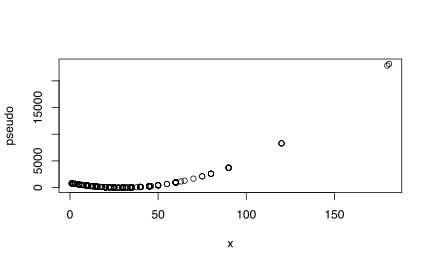
\includegraphics[width=0.7\linewidth]{Notas-Curso-Estadistica_files/figure-latex/unnamed-chunk-81-1} \end{center}

Con estos pseudo-valores, es posible estimar la media y la varianza de
\(T_{n}\) con los siguientes estimadores respectivos:

\[
T_{\text {jack }}=\frac{1}{n} \sum_{i=1}^{n} \widetilde{T}_{i}
\]

y

\[
v_{jack}=\frac{\sum_{i=1}^{n}\left(\widetilde{T}_{i}-\frac{1}{n}
\sum_{i=1}^{n} \widetilde{T}_{i}\right)^{2}}{n-1}.
\]

\begin{remark}
Sin embargo, se puede demostrar fácilmente que se pueden usar
pseudovalores para construir una prueba normal de hipótesis.

Como los pseudovalores son idénticamente distribuidos entonces su promedio se ajusta de forma aproximada a una distribución normal a medida
que el tamaño de la muestra aumenta. Por lo tanto, tenemos que
\[
  \frac{\sqrt{n}\left(T_{jack}-\theta\right)}{\sqrt{v_{jack}}}
  \rightarrow N(0,1).
\]
\end{remark}

\begin{Shaded}
\begin{Highlighting}[]
\NormalTok{(Tjack }\OtherTok{\textless{}{-}} \FunctionTok{mean}\NormalTok{(pseudo))}
\end{Highlighting}
\end{Shaded}

\begin{verbatim}
## [1] 429.2484
\end{verbatim}

\begin{Shaded}
\begin{Highlighting}[]
\NormalTok{(Vjack }\OtherTok{\textless{}{-}} \FunctionTok{var}\NormalTok{(pseudo, }\AttributeTok{na.rm =} \ConstantTok{TRUE}\NormalTok{))}
\end{Highlighting}
\end{Shaded}

\begin{verbatim}
## [1] 2701991
\end{verbatim}

\begin{Shaded}
\begin{Highlighting}[]
\NormalTok{(sdjack }\OtherTok{\textless{}{-}} \FunctionTok{sqrt}\NormalTok{(Vjack))}
\end{Highlighting}
\end{Shaded}

\begin{verbatim}
## [1] 1643.774
\end{verbatim}

\begin{Shaded}
\begin{Highlighting}[]
\NormalTok{(z }\OtherTok{\textless{}{-}} \FunctionTok{qnorm}\NormalTok{(}\DecValTok{1} \SpecialCharTok{{-}} \FloatTok{0.05}\SpecialCharTok{/}\DecValTok{2}\NormalTok{))}
\end{Highlighting}
\end{Shaded}

\begin{verbatim}
## [1] 1.959964
\end{verbatim}

\begin{Shaded}
\begin{Highlighting}[]
\FunctionTok{c}\NormalTok{(Tjack }\SpecialCharTok{{-}}\NormalTok{ z }\SpecialCharTok{*}\NormalTok{ sdjack}\SpecialCharTok{/}\FunctionTok{sqrt}\NormalTok{(n), Tjack }\SpecialCharTok{+}\NormalTok{ z }\SpecialCharTok{*}\NormalTok{ sdjack}\SpecialCharTok{/}\FunctionTok{sqrt}\NormalTok{(n))}
\end{Highlighting}
\end{Shaded}

\begin{verbatim}
## [1] 285.1679 573.3289
\end{verbatim}

\hypertarget{bootstrap}{%
\section{Bootstrap}\label{bootstrap}}

Este método es un poco más sencillo de implementar que Jackknife y es
igualmente de eficaz. Este fue propuesto por Bradley Efron en \autocite{Efron1979}.

Primero recordemos que estamos estimando la variabilidad propia de un estadístico a partir de
una muestra. Asuma que este estadístico tiene la forma \(T_{n}=g\left( X_{1},\ldots,X_{n} \right)\)
donde \(g\) es cualquier función (media, varianza, quantiles, etc).

Supongamos que conocemos la distribución real de los \(X\)'s, llamada \(F(x)\) y asumamos que \(T_n=\bar X_n\). Si uno
quisiera estimar la varianza de \(T_n\) basta con hacer

\begin{equation*}
\mathbb{V}_{F}\left(T_{n}\right):=\mathrm{Var}_{F}\left(T_{n}\right)
= \frac{\sigma^{2}}{n}=\frac{\int x^{2}  dF(x)-\left(\int x
dF(x)\right)^{2}}{n}
\end{equation*}

donde \(\sigma^{2} = \mathrm{Var}\left(X\right)\) y el subindice \(F\) es solo para indicar la dependencia con la distribución real.

Ahora dado que no tenemos la distribución real \(F(x)\), una opción es utilizar el estimador empírico \(\hat{F}_n\) como estimador plug-in en la formulación de la varianza de \(T_n\).

De manera sencilla se puede resumir la técnica de bootstrap como una simulación iid de la distribución \(\hat{F}_n\) de modo que se pueda conocer la varianza del estadístico \(T_n\).

En simples pasos la técnica es

\begin{enumerate}
\def\labelenumi{\arabic{enumi}.}
\tightlist
\item
  Seleccione \(X_{1}^{*}, \ldots, X_{n}^{*} \sim \widehat{F}_{n}\)
\item
  Estime \(T_{n}^{*}=g\left(X_{1}^{*}, \ldots, X_{n}^{*}\right)\)
\item
  Repita los Pasos 1 y 2, \(B\) veces para obtener \(T_{n, 1}^{*}, \ldots, T_{n, B}^{*}\)
\item
  Estime
  \[
  v_{\mathrm{boot}}=\frac{1}{B} \sum_{b=1}^{B}\left(T_{n, b}^{*}-\frac{1}{B} \sum_{r=1}^{B} T_{n, r}^{*}\right)^{2}
  \]
\end{enumerate}

Por la ley de los grandes números tenemos que

\begin{equation}
v_{\mathrm{boot}} \stackrel{\mathrm{a.s.}}{\longrightarrow} \mathbb{V}_{\widehat{F}_{n}}\left(T_{n}\right), \quad  \text{si} \quad B\rightarrow \infty.
\end{equation}

además llamaremos,

\begin{equation*}
\widehat{\mathrm{se}}_{\mathrm{boot}}=\sqrt{v_{\mathrm{boot}}}
\end{equation*}

En pocas palabras lo que tenemos es que

\begin{align*}
\text  {Mundo Real: }
& F
& \Longrightarrow  X_{1}, \ldots, X_{n}
& \Longrightarrow
& T_{n} = g\left(X_{1}, \ldots, X_{n}\right) \\
\text {Mundo Bootstrap: }
& \widehat{F}_{n}
& \Longrightarrow  X_{1}^{*}, \ldots, X_{n}^{*}
& \Longrightarrow
& T_{n}^{*}=g\left(X_{1}^{*}, \ldots, X_{n}^{*}\right)
\end{align*}

En términos de convergencia lo que se tiene es que
\[
\mathrm{Var}_{F}\left(T_{n}\right) \overbrace{\approx}^{O(1 / \sqrt{n})} \mathrm{Var}_{\widehat{F}_{n}}\left(T_{n}\right) \overbrace{\approx}^{O(1 / \sqrt{B})} v_{b o o t}
\]

producto de la ley de grandes números en ambos casos.

\begin{remark}
¿Cómo extraemos una muestra de \(\hat{F}_n\)?
\end{remark}

Recuerden que \(\hat{F}_{n}\) asigna la probabilidad de \(\frac{1}{n}\) a cada valor usado para construirla.

Por lo tanto, todos los puntos originales \(X_{1},\ldots,X_{n}\) tienen probabilidad \(\frac{1}{n}\) de ser escogidos, que resulta ser equivalente a un muestreo con remplazo \(n\)-veces.

Así que basta cambiar el punto 1. del algoritmo mencionando anteriormente con

\begin{enumerate}
\def\labelenumi{\arabic{enumi}.}
\tightlist
\item
  Seleccione una muestra con remplazo \(X_{1}^{*}, \ldots, X_{n}^{*}\) de \(X_{1},\ldots,X_{n}\).
\end{enumerate}

\begin{exercise}
\protect\hypertarget{exr:unnamed-chunk-89}{}\label{exr:unnamed-chunk-89}En este ejemplo podemos tomar \(B=1000\) y construir esa cantidad de veces nuestro estimador de varianza:
\end{exercise}

\begin{Shaded}
\begin{Highlighting}[]
\NormalTok{B }\OtherTok{\textless{}{-}} \DecValTok{1000}
\NormalTok{Tboot\_b }\OtherTok{\textless{}{-}} \ConstantTok{NULL}

\ControlFlowTok{for}\NormalTok{ (b }\ControlFlowTok{in} \DecValTok{1}\SpecialCharTok{:}\NormalTok{B) \{}
\NormalTok{    xb }\OtherTok{\textless{}{-}} \FunctionTok{sample}\NormalTok{(x, }\AttributeTok{size =}\NormalTok{ n, }\AttributeTok{replace =} \ConstantTok{TRUE}\NormalTok{)}
\NormalTok{    Tboot\_b[b] }\OtherTok{\textless{}{-}} \FunctionTok{var}\NormalTok{(xb)}
\NormalTok{\}}

\NormalTok{Tboot\_b[}\DecValTok{1}\SpecialCharTok{:}\DecValTok{10}\NormalTok{]}
\end{Highlighting}
\end{Shaded}

\begin{verbatim}
##  [1] 345.1819 493.5279 273.3998 446.3071 426.0340 384.2662 383.2132 455.8139
##  [9] 462.3363 594.5774
\end{verbatim}

\begin{Shaded}
\begin{Highlighting}[]
\FunctionTok{plot}\NormalTok{(Tboot\_b)}
\end{Highlighting}
\end{Shaded}

\begin{center}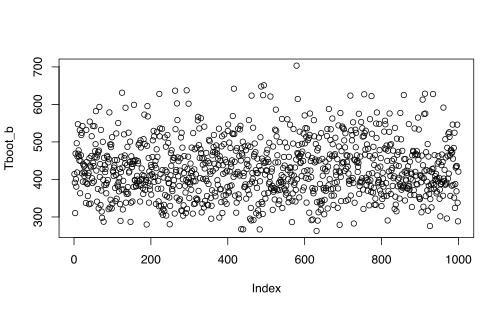
\includegraphics[width=0.7\linewidth]{Notas-Curso-Estadistica_files/figure-latex/unnamed-chunk-91-1} \end{center}

\begin{Shaded}
\begin{Highlighting}[]
\FunctionTok{hist}\NormalTok{(Tboot\_b)}
\end{Highlighting}
\end{Shaded}

\begin{center}\includegraphics[width=0.7\linewidth]{Notas-Curso-Estadistica_files/figure-latex/unnamed-chunk-91-2} \end{center}

Por supuesto podemos encontrar los estadísticos usuales para esta nueva muestra

\begin{Shaded}
\begin{Highlighting}[]
\NormalTok{(Tboot }\OtherTok{\textless{}{-}} \FunctionTok{mean}\NormalTok{(Tboot\_b))}
\end{Highlighting}
\end{Shaded}

\begin{verbatim}
## [1] 428.066
\end{verbatim}

\begin{Shaded}
\begin{Highlighting}[]
\NormalTok{(Vboot }\OtherTok{\textless{}{-}} \FunctionTok{var}\NormalTok{(Tboot\_b))}
\end{Highlighting}
\end{Shaded}

\begin{verbatim}
## [1] 5504.701
\end{verbatim}

\begin{Shaded}
\begin{Highlighting}[]
\NormalTok{(sdboot }\OtherTok{\textless{}{-}} \FunctionTok{sqrt}\NormalTok{(Vboot))}
\end{Highlighting}
\end{Shaded}

\begin{verbatim}
## [1] 74.19367
\end{verbatim}

\begin{remark}
Si \(\hat \theta\) es un estimador de \(\theta\) (bajo cualquier método) entonces podemos sustituir el paso 1 en el algoritmo de Bootstrap por lo siguiente:

\begin{enumerate}
\def\labelenumi{\arabic{enumi}.}
\tightlist
\item
  Seleccione \(X_{1}^{*}, \ldots, X_{n}^{*} \sim F_{\hat \theta}\)
\end{enumerate}

A este algoritmo modificado le llamamos Bootstrap paramétrico.
\end{remark}

\hypertarget{intervalos-de-confianza}{%
\subsection{Intervalos de confianza}\label{intervalos-de-confianza}}

\hypertarget{intervalo-normal}{%
\subsubsection{Intervalo Normal}\label{intervalo-normal}}

Este es el más sencillo y se escribe como

\begin{equation}
T_{n} \pm z_{\alpha / 2} \widehat{\mathrm{Se}}_{\mathrm{boot}}
\end{equation}

\begin{remark}
Este intervalo solo funciona si la distribución de \(T_{n}\) es normal.
\end{remark}

El cálculo de este intervalo es

\begin{Shaded}
\begin{Highlighting}[]
\FunctionTok{c}\NormalTok{(Tn }\SpecialCharTok{{-}}\NormalTok{ z }\SpecialCharTok{*}\NormalTok{ sdboot, Tn }\SpecialCharTok{+}\NormalTok{ z }\SpecialCharTok{*}\NormalTok{ sdboot)}
\end{Highlighting}
\end{Shaded}

\begin{verbatim}
## [1] 283.8315 574.6653
\end{verbatim}

\hypertarget{intervalo-pivotal}{%
\subsubsection{Intervalo pivotal}\label{intervalo-pivotal}}

Sea \(\theta=T(F)\) y \(\widehat{\theta}_{n}=T\left(\widehat{F}_{n}\right)\) y defina la cantidad pivotal \(R_{n}=\widehat{\theta}_{n}-\theta .\)

Sea \(H(r)\) la función de distribución del pivote:
\[
H(r)=\mathbb{P}_{F}\left(R_{n} \leq r\right).
\]

Además considere \(C_{n}^{\star}=(a, b)\) donde
\[
a=\widehat{\theta}_{n}-H^{-1}\left(1-\frac{\alpha}{2}\right) \quad \text { y } \quad b=\widehat{\theta}_{n}-H^{-1}\left(\frac{\alpha}{2}\right).
\]

Se sigue que
\begin{align*}
\mathbb{P}(a \leq \theta \leq b)
&=\mathbb{P}\left(\widehat{\theta}_{n}-b \leq R_{n} \leq \widehat{\theta}_{n}-a\right) \\
&=H\left(\widehat{\theta}_{n}-a\right)-H\left(\widehat{\theta}_{n}-b\right) \\
&=H\left(H^{-1}\left(1-\frac{\alpha}{2}\right)\right)-H\left(H^{-1}\left(\frac{\alpha}{2}\right)\right) \\
&=1-\frac{\alpha}{2}-\frac{\alpha}{2}=1-\alpha
\end{align*}

\begin{remark}
\(C_{n}^{\star}=(a, b)\) es un intervalo de confianza al (\(1-\alpha\))\%.

El problema es que este intervalo depende de \(H\) desconocido.
\end{remark}

Para resolver este problema, se puede construir una versión \emph{bootstrap} de \(H\) usando lo que sabemos hasta ahora:

\[
\widehat{H}(r)=\frac{1}{B} \sum_{b=1}^{B} I\left(R_{n, b}^{*} \leq r\right)
\]
donde \(R_{n, b}^{*}=\widehat{\theta}_{n, b}^{*}-\widehat{\theta}_{n}\).

Sea \(r_{\beta}^{*}\) el cuantil muestral de tamaño \(\beta\) de \(\left(R_{n, 1}^{*}, \ldots, R_{n, B}^{*}\right)\) y sea \(\theta_{\beta}^{*}\) el cuantil muestral de tamaño \(\beta\) de \(\left(\theta_{n, 1}^{*}, \ldots, \theta_{n, B}^{*}\right)\).

\begin{remark}
Según la notación anterior se cumple que:
\begin{equation*}
r_{\beta}^{*}= \theta_{\beta}^{*}-\widehat{\theta}_{n}
\end{equation*}
\end{remark}

A partir de loa estadísticos anteriores se puede construir un intervalo de confianza aproximado \(C_{n}=(\widehat{a}, \widehat{b})\) al (\(1-\alpha\))\% donde:

\begin{align*}
\widehat{a}&= \widehat{\theta}_{n}-\widehat{H}^{-1}\left(1-\frac{\alpha}{2}\right) = \widehat{\theta}_{n}-r_{1-\alpha / 2}^{*} = \widehat{\theta}_{n}-\theta_{1-\alpha / 2}^{*} + \widehat{\theta}_{n} =2 \widehat{\theta}_{n}-\theta_{1-\alpha / 2}^{*} \\
\widehat{b} &=\widehat{\theta}_{n}-\widehat{H}^{-1}\left(\frac{\alpha}{2}\right)
=\widehat{\theta}_{n}-r_{\alpha / 2}^{*}
= \widehat{\theta}_{n}-\theta_{\alpha / 2}^{*} + \widehat{\theta}_{n}
=2 \widehat{\theta}_{n}-\theta_{\alpha / 2}^{*}
\end{align*}

\begin{remark}
El intervalo de confianza pivotal de tamaño \(1-\alpha\) es
\[
  C_{n}=\left(2 \widehat{\theta}_{n}-\widehat{\theta}_{((1-\alpha / 2) B)}^{*}, 2 \widehat{\theta}_{n}-\widehat{\theta}_{((\alpha / 2) B)}^{*}\right)
  \]
\end{remark}

El intervalo anterior para un nivel de 95\% se estima de la siguiente forma

\begin{Shaded}
\begin{Highlighting}[]
\FunctionTok{c}\NormalTok{(}\DecValTok{2} \SpecialCharTok{*}\NormalTok{ Tn }\SpecialCharTok{{-}} \FunctionTok{quantile}\NormalTok{(Tboot\_b, }\DecValTok{1} \SpecialCharTok{{-}} \FloatTok{0.05}\SpecialCharTok{/}\DecValTok{2}\NormalTok{), }\DecValTok{2} \SpecialCharTok{*}\NormalTok{ Tn }\SpecialCharTok{{-}}
    \FunctionTok{quantile}\NormalTok{(Tboot\_b, }\FloatTok{0.05}\SpecialCharTok{/}\DecValTok{2}\NormalTok{))}
\end{Highlighting}
\end{Shaded}

\begin{verbatim}
##    97.5%     2.5% 
## 267.1250 552.9294
\end{verbatim}

\hypertarget{intervalo-pivotal-studentizado}{%
\subsubsection{Intervalo pivotal studentizado}\label{intervalo-pivotal-studentizado}}

Una versión mejorada del intervalo pivotal sería a través de la normalización de los estimadores de \(T_n\):

\[
Z_{n}=\frac{T_{n}-\theta}{\widehat{\mathrm{se}}_{\mathrm{boot}}}.
\]
Como \(\theta\) es desconocido, entonces la versión a estimar es
\[
Z_{n, b}^{*}=\frac{T_{n, b}^{*}-T_{n}}{\widehat{\mathrm{se}}_{b}^{*}}
\]
donde \(\widehat{\mathrm{se}}_{b}^{*}\) es un estimador del error estándar de \(T_{n, b}^{*}\) no de \(T_{n}\).

\begin{remark}
Para calcular \(Z_{n, b}^{*}\) requerimos estimar la varianza de \(T_{n,b}^*\) para cada \(b\).
\end{remark}

Con esto se puede obtener cantidades \(Z_{n, 1}^{*}, \ldots, Z_{n, B}^{*}\) que debería ser próximos a \(Z_{n}\). (Bootstrap de los estadísticos normalizados)

Sea \(z_{\alpha}^{*}\) el \(\alpha\)-cuantil de \(Z_{n, 1}^{*}, \ldots, Z_{n, B}^{*},\) entonces \(\mathbb{P}\left(Z_{n} \leq z_{\alpha}^{*}\right) \approx \alpha\).

Define el intervalo
\begin{equation*}
C_{n}=\left(T_{n}-z_{1-\alpha / 2}^{*} \widehat{\mathrm{se}}_{\mathrm{boot}}, T_{n}-z_{\alpha / 2}^{*} \widehat{\mathrm{se}}_{\mathrm{boot}}\right)
\end{equation*}

Justificado por el siguiente cálculo:

\begin{align*}
\mathbb{P}\left(\theta \in C_{n}\right) &=\mathbb{P}\left(T_{n}-z_{1-\alpha / 2}^{*} \widehat{\mathrm{Se}}_{\mathrm{boot}} \leq \theta \leq T_{n}-z_{\alpha / 2}^{*} \widehat{\mathrm{Se}}_{\mathrm{boot}}\right) \\
&=\mathbb{P}\left(z_{\alpha / 2}^{*} \leq \frac{T_{n}-\theta}{\mathrm{se}_{\mathrm{boot}}} \leq z_{1-\alpha / 2}^{*}\right) \\
&=\mathbb{P}\left(z_{\alpha / 2}^{*} \leq Z_{n} \leq z_{1-\alpha / 2}^{*}\right) \\
& \approx 1-\alpha
\end{align*}

Note que para este caso tenemos que hacer bootstrap para cada estimador bootstrap calculado.

\begin{Shaded}
\begin{Highlighting}[]
\NormalTok{B }\OtherTok{\textless{}{-}} \DecValTok{1000}
\NormalTok{Tboot\_b }\OtherTok{\textless{}{-}} \ConstantTok{NULL}
\NormalTok{Tboot\_bm }\OtherTok{\textless{}{-}} \ConstantTok{NULL}
\NormalTok{sdboot\_b }\OtherTok{\textless{}{-}} \ConstantTok{NULL}

\ControlFlowTok{for}\NormalTok{ (b }\ControlFlowTok{in} \DecValTok{1}\SpecialCharTok{:}\NormalTok{B) \{}
\NormalTok{    xb }\OtherTok{\textless{}{-}} \FunctionTok{sample}\NormalTok{(x, }\AttributeTok{size =}\NormalTok{ n, }\AttributeTok{replace =} \ConstantTok{TRUE}\NormalTok{)}
\NormalTok{    Tboot\_b[b] }\OtherTok{\textless{}{-}} \FunctionTok{var}\NormalTok{(xb)}
    \ControlFlowTok{for}\NormalTok{ (m }\ControlFlowTok{in} \DecValTok{1}\SpecialCharTok{:}\NormalTok{B) \{}
\NormalTok{        xbm }\OtherTok{\textless{}{-}} \FunctionTok{sample}\NormalTok{(xb, }\AttributeTok{size =}\NormalTok{ n, }\AttributeTok{replace =} \ConstantTok{TRUE}\NormalTok{)}
\NormalTok{        Tboot\_bm[m] }\OtherTok{\textless{}{-}} \FunctionTok{var}\NormalTok{(xbm)}
\NormalTok{    \}}
\NormalTok{    sdboot\_b[b] }\OtherTok{\textless{}{-}} \FunctionTok{sd}\NormalTok{(Tboot\_bm)}
\NormalTok{\}}

\NormalTok{z\_star }\OtherTok{\textless{}{-}}\NormalTok{ (Tboot\_b }\SpecialCharTok{{-}}\NormalTok{ Tn)}\SpecialCharTok{/}\NormalTok{sdboot\_b}

\FunctionTok{hist}\NormalTok{(z\_star)}
\end{Highlighting}
\end{Shaded}

\begin{center}\includegraphics[width=0.7\linewidth]{Notas-Curso-Estadistica_files/figure-latex/unnamed-chunk-103-1} \end{center}

\begin{Shaded}
\begin{Highlighting}[]
\FunctionTok{c}\NormalTok{(Tn }\SpecialCharTok{{-}} \FunctionTok{quantile}\NormalTok{(z\_star, }\DecValTok{1} \SpecialCharTok{{-}} \FloatTok{0.05}\SpecialCharTok{/}\DecValTok{2}\NormalTok{) }\SpecialCharTok{*}\NormalTok{ sdboot, Tn }\SpecialCharTok{{-}}
    \FunctionTok{quantile}\NormalTok{(z\_star, }\FloatTok{0.05}\SpecialCharTok{/}\DecValTok{2}\NormalTok{) }\SpecialCharTok{*}\NormalTok{ sdboot)}
\end{Highlighting}
\end{Shaded}

\begin{verbatim}
##    97.5%     2.5% 
## 317.7259 707.0044
\end{verbatim}

\hypertarget{resumiendo}{%
\subsection{Resumiendo}\label{resumiendo}}

Resumiendo todos lo métodos de cálculo de intervalos obtenemos

\begin{Shaded}
\begin{Highlighting}[]
\NormalTok{knitr}\SpecialCharTok{::}\FunctionTok{kable}\NormalTok{(}\FunctionTok{data.frame}\NormalTok{(}\AttributeTok{Metodo =} \FunctionTok{c}\NormalTok{(}\StringTok{"Jackknife"}\NormalTok{, }\StringTok{"Bootstrap Normal"}\NormalTok{,}
    \StringTok{"Bootstrap Pivotal"}\NormalTok{, }\StringTok{"Bootstrap Pivotal Estudentizado"}\NormalTok{),}
    \AttributeTok{Inferior =} \FunctionTok{c}\NormalTok{(Tjack }\SpecialCharTok{{-}}\NormalTok{ z }\SpecialCharTok{*}\NormalTok{ sdjack}\SpecialCharTok{/}\FunctionTok{sqrt}\NormalTok{(n), Tn }\SpecialCharTok{{-}}\NormalTok{ z }\SpecialCharTok{*}
\NormalTok{        sdboot, }\DecValTok{2} \SpecialCharTok{*}\NormalTok{ Tn }\SpecialCharTok{{-}} \FunctionTok{quantile}\NormalTok{(Tboot\_b, }\DecValTok{1} \SpecialCharTok{{-}} \FloatTok{0.05}\SpecialCharTok{/}\DecValTok{2}\NormalTok{),}
\NormalTok{        Tn }\SpecialCharTok{{-}} \FunctionTok{quantile}\NormalTok{(z\_star, }\DecValTok{1} \SpecialCharTok{{-}} \FloatTok{0.05}\SpecialCharTok{/}\DecValTok{2}\NormalTok{) }\SpecialCharTok{*}\NormalTok{ sdboot),}
    \AttributeTok{Superior =} \FunctionTok{c}\NormalTok{(Tjack }\SpecialCharTok{+}\NormalTok{ z }\SpecialCharTok{*}\NormalTok{ sdjack}\SpecialCharTok{/}\FunctionTok{sqrt}\NormalTok{(n), Tn }\SpecialCharTok{+}\NormalTok{ z }\SpecialCharTok{*}
\NormalTok{        sdboot, }\DecValTok{2} \SpecialCharTok{*}\NormalTok{ Tn }\SpecialCharTok{{-}} \FunctionTok{quantile}\NormalTok{(Tboot\_b, }\FloatTok{0.05}\SpecialCharTok{/}\DecValTok{2}\NormalTok{),}
\NormalTok{        Tn }\SpecialCharTok{{-}} \FunctionTok{quantile}\NormalTok{(z\_star, }\FloatTok{0.05}\SpecialCharTok{/}\DecValTok{2}\NormalTok{) }\SpecialCharTok{*}\NormalTok{ sdboot)))}
\end{Highlighting}
\end{Shaded}

\begin{tabular}{l|r|r}
\hline
Metodo & Inferior & Superior\\
\hline
Jackknife & 285.1679 & 573.3289\\
\hline
Bootstrap Normal & 283.8315 & 574.6653\\
\hline
Bootstrap Pivotal & 271.2827 & 551.4989\\
\hline
Bootstrap Pivotal Estudentizado & 317.7259 & 707.0044\\
\hline
\end{tabular}

\hypertarget{ejercicios-1}{%
\section{Ejercicios}\label{ejercicios-1}}

\begin{enumerate}
\def\labelenumi{\arabic{enumi}.}
\item
  Repita los ejercicios anteriores para calcular intervalos de confianza para la distancia promedio y la varianza del desplazamiento de las personas. Use los métodos de Jackknife y Bootstrap (con todos sus intervalos de confianza).
  Dada que la distancia es una medida que puede ser influenciada por distancias muy cortas o muy largas, se puede calcular el logaritmo de esta variable para eliminar la escala de la distancias.
\item
  Verifique que esta última variable se podría estimar paramétricamente con una distribución normal.
  Repita los cálculos anteriores tomando como cuantiles los de una normal con media 0 y varianza 1.
\item
  Compare los intervalos calculados y comente los resultados.
\item
  Del libro \autocite{Wasserman2006} \textbf{Sección 3:} 2, 3, 7, 9, 11.
\end{enumerate}

\hypertarget{muxe9todos-lineales-de-regresiuxf3n}{%
\chapter{Métodos lineales de regresión}\label{muxe9todos-lineales-de-regresiuxf3n}}

\textbf{NOTA: Para los siguientes capítulos nos basaremos en los libros \autocite{HastieElements2009} y \autocite{James2013b}.}

\hypertarget{introducciuxf3n-al-aprendizaje-estaduxedstico.}{%
\section{Introducción al Aprendizaje Estadístico.}\label{introducciuxf3n-al-aprendizaje-estaduxedstico.}}

Supongamos que tenemos \(p\) variables de entrada que provocan una respuesta \(Y\) (variable dependiente) a través de la siguiente relación:

\begin{equation}
Y = f(X_{1},\ldots,X_{p}) + \varepsilon
\label{eq:regresion-general}
\end{equation}
donde \(f\) es desconocida, las variables \(X\)'s son las variables de entrada (covariables o predictores) y \(\varepsilon\) representa un error aditivo a la relación definida por \(f\).

Hay dos motivos por los que estimamos \(f\):

\begin{enumerate}
\def\labelenumi{\arabic{enumi}.}
\tightlist
\item
  \textbf{Predicción:} Si se estima \(f\) con \(\hat{f}\) entonces
  \begin{equation*}
  \hat{Y} = \hat{f}(X_{1},\ldots,X_{p}). 
  \end{equation*}
  asumiendo que el valor medio del error \(\epsilon\) es cero. Si tuvieramos valores nuevos de los \(X\)'s entonces podríamos estimar el valor que el corresponde a \(Y\).
\end{enumerate}

En este caso obtener una estructura óptima o precisa de la función \(\hat f\) no es importante, siempre y cuando sea posible obtener buenas predicciones de \(Y\). Para entender mejor esta idea se puede definir:

\begin{enumerate}
\def\labelenumi{\alph{enumi}.}
\tightlist
\item
  \textbf{Error reducible:} Error de \(\hat{f}\) alrededor de \(f\), el cual es propio de la escogencia del modelo.
\item
  \textbf{Error irreducible:} Error que escapa a una estimación perfecta de \(f\). Puede venir de covariables no consideradas en el problema, fuentes de error que no se pueden cuantificar, etc.
\end{enumerate}

\begin{align*}
\mathbb{E}\left[(\hat{Y}-Y\right)^2] 
&=  \mathbb{E}\left[\left(  f(X_{1},\ldots,X_{p}) + \varepsilon - \hat{f}(X_{1},\ldots,X_{p}) \right)^{2}  \right] \\
&= \underbrace{\left( f(X_{1},\ldots,X_{p})- \hat{f}(X_{1},\ldots,X_{p})  \right) ^{2} }_{\text{Reducible}}
+\underbrace{\mathrm{Var}\left(\varepsilon\right)}_{\text{irreducible}}.
\end{align*}
asumiendo que \(f\) y \(X\) son conocidas y determinísticas.

\begin{enumerate}
\def\labelenumi{\arabic{enumi}.}
\setcounter{enumi}{1}
\tightlist
\item
  \textbf{Inferencia:} Entender la relación entre \(X\) y \(Y\), es decir entender cómo \(Y\) cambia como función de las covariables.
  En este caso sí nos interesa obtener un estimador preciso e interpretable de la función \(f\). Las siguientes preguntas son de interés:
\end{enumerate}

\begin{itemize}
\tightlist
\item
  ¿Cuáles covariables están asociadas con la variable respuesta o dependiente?
\item
  ¿Cuál es la relación entre cada variable predictora y la respuesta?
\item
  ¿La relación entre covariables y variable dependiente es lineal? o ¿la relación es más compleja?
\end{itemize}

\hypertarget{formas-de-estimar-f}{%
\subsection{\texorpdfstring{Formas de estimar \(f\)}{Formas de estimar f}}\label{formas-de-estimar-f}}

El proceso de estimación de \(f\) a través de \(\hat f\) se realiza sobre un subconjunto de los datos disponibles. A este conjunto se le llama \emph{datos de entrenamiento}. El resto de los datos se puede utilizar para probar la capacidad predictiva del modelo seleccionado.

Existen varias clasificaciones de modelos para estimar \(f\):

\begin{itemize}
\tightlist
\item
  Modelos paramétricos vs modelos no parámetricos. Los modelos pueden tener parámetros que facilitan el proceso de estimación, pero el número de parámetros debe ser conservador para evitar situaciones de \emph{sobreajuste}. Los modelos no-paramétricos requieren de mucha información para dar un buen ajuste, sea a través de una muestra grande o a través de manipular parámetros generales de suavidad (ancho de banda).
\item
  Modelos predictivos vs modelos interpretativos. Entre más flexible (complejo) sea un modelo, más dificil es su interpretación, por lo tanto más dificil es hacer inferencia. Hay modelos muy flexibles que permiten hacer muy buena predicción, pero fácilmente se puede caer en sobreajuste.
\item
  Modelos supervisados vs no supervisados. ¿La variable \(Y\) está disponible en la muestra?
\item
  Modelos de regresión vs modelos de clasificación. ¿La variable \(Y\) es continua o es una variable categórica?
\end{itemize}

\hypertarget{medidas-de-bondad-de-ajuste}{%
\subsection{Medidas de bondad de ajuste}\label{medidas-de-bondad-de-ajuste}}

En el caso de regresión, la medida más utilizada es el Error Cuadrático Medio (MSE):
\begin{align*}
MSE=\frac 1 n \sum_{i=1}^n(y_i-\hat f(x_i))^2
\end{align*}
calculada sobre la base de entrenamiento del modelo para evaluar la capacidad de ajuste de \(\hat f\). Para evaluar la capacidad predictiva del modelo se puede usar el mismo concepto sobre la \emph{base de prueba}. La diferencia entre la magnitud del MSE en los dos conjuntos de datos, puede ser un indicador de sobreajuste.

Para el caso de un problema de aprendizaje estadístico hay interpretaciones de los componentes de sesgo y varianza:

\begin{itemize}
\tightlist
\item
  \emph{Varianza}: variación de \(\hat f\) ante cambios en los datos de entrenamiento. Modelos más flexibles tienen mayor varianza.
\item
  \emph{Sesgo}: error al aproximar la realidad complicada con un modelo más simple. Modelos más flexibles tienen menor sesgo.
\end{itemize}

\textbf{Estrategia de búsqueda de modelos}: conforme aumenta la flexibilidad de un modelo el sesgo disminuye, y la varianza no aumenta en el mismo ritmo. A partir de un cierto momento la disminución del sesgo no es lo suficientemente fuerte como para contrarrestar el crecimiento en varianza.

\textbf{Conclusión}: un modelo parsimonioso posiblemente garantizará un valor óptimo en MSE.

\hypertarget{regresiuxf3n-lineal}{%
\section{Regresión lineal}\label{regresiuxf3n-lineal}}

El caso más sencillo es cuando se asume que la relación es lineal y se describe de la siguiente forma:

\begin{equation*}
Y = \beta_{0} + \beta_{1}X_{1} + \cdots +  \beta_{p}X_{p} + \varepsilon.
\end{equation*}

Aquí los valores \(\beta\)'s son constantes a estimar, las variables \(X\)'s son las variables de entrada y \(\varepsilon\) es el error irreducible cometido por hacer esta aproximación.

Las covariables en un modelo de regresión pueden ser:

\begin{enumerate}
\def\labelenumi{\arabic{enumi}.}
\tightlist
\item
  Cuantitativas: variables continuas.
\item
  Categóricas: variables tipo factor que admiten un número de niveles. Estas variables pueden ser ordinales o nominales, dependiendo si hay un orden natural en la escala de los niveles. Para incorporarla en el modelo de regresión debemos \emph{codificar} la variable:
\end{enumerate}

\begin{example}
\protect\hypertarget{exm:unnamed-chunk-107}{}\label{exm:unnamed-chunk-107}Se tiene la variable \(G\) codificada con Casado (1), Soltero (2), Divorciado (3) y Unión Libre (4). Si queremos incorporar esta variable en una regresión podríamos usar la siguiente codificación:

\begin{equation*}
X_{j} = \mathbf{1}_{\{G=j+1\}} 
\end{equation*}

que resulta en la matriz

\begin{equation*}
\begin{matrix}
X_{1} & X_{2} & X_{3}\\
0 & 0 & 0 \\
1 & 0 & 0 \\
0 & 1 & 0 \\
0 & 0 & 1 \\
\end{matrix}
\end{equation*}

Existen otras formas de codificar este tipo de variables, pero esta es una de las más usuales.
\end{example}

\hypertarget{forma-matricial}{%
\subsection{Forma matricial}\label{forma-matricial}}

Podemos escribir el modelo de regresión en forma matricial:

\begin{equation*}
\boldsymbol{Y} = \boldsymbol{X}\boldsymbol{\beta} + \boldsymbol{\varepsilon}
\end{equation*}

donde

\begin{multline*}
\boldsymbol{Y} = 
\begin{pmatrix}
Y_{1} \\
\vdots \\
Y_{n}
\end{pmatrix}_{n\times 1} 
\quad 
\boldsymbol{X} = 
\begin{pmatrix}
1 & X_{1,1} & \cdots & X_{p,1} \\
\vdots & \vdots & \cdots & \vdots\\
1 & X_{1,n}& \cdots & X_{p,n}
\end{pmatrix}_{n\times (p+1)}
\\
\boldsymbol{\varepsilon} = 
\begin{pmatrix}
\varepsilon_{1} \\
\vdots \\
\varepsilon_{n}
\end{pmatrix}_{n\times 1} 
\quad 
\boldsymbol{\beta} = 
\begin{pmatrix}
\beta_{0} \\
\beta_{1} \\
\vdots \\
\beta_{p}
\end{pmatrix}_{(p+1)\times 1} 
\end{multline*}

Suponemos que \(\mathbb{E}\left[\varepsilon_{i}\right] = 0\) y \(\mathrm{Var}\left(\varepsilon_{i}\right) = \sigma^{2}\).

La forma de resolver este problema es por minimos cuadrados. Es decir, buscamos el \(\hat{\beta}\) que cumpla lo siguiente:

\begin{align}
\hat{\beta} &= 
 \operatorname{argmin}_\beta (\boldsymbol{Y} - \boldsymbol{X} \boldsymbol{\beta})^{\top} (\boldsymbol{Y} - \boldsymbol{X} \boldsymbol{\beta})\\
 &=  \operatorname{argmin}_\beta \sum_{i=1}^n \left( Y_{i} -\beta_{0} - \sum_{j=1}^p X_{j,i} \beta_{j} \right)^2 
 \label{eq:minimos-cuadrados}
 \end{align}

\includegraphics{manual_figures/ols.png}
Por lo tanto buscaríamos minimizar la suma de \emph{residuos} al cuadrado.

Suponga que \(\gamma\) es un vector cualquiera en \(\mathbb{R}^{p+1}\) y defina \(V := \{\boldsymbol{X}\boldsymbol{\gamma}, \gamma \in \mathbb{R}^{p+1}\}\), es decir el espacio lineal generado por las columnas (covariables) de \(\boldsymbol{X}\). Buscamos entonces un vector \(\beta\) que cumpla:

\begin{align*}
\boldsymbol{X}\boldsymbol{\beta}
 &= \operatorname{Proy}_{V} \boldsymbol{Y}
\end{align*}

Entonces dado que \(\boldsymbol{Y}-\boldsymbol{X}\boldsymbol{\beta} \perp V\), es decir \(\boldsymbol{Y}-\boldsymbol{X}\boldsymbol{\beta} \perp \boldsymbol{X}\boldsymbol{\gamma}, \forall \boldsymbol{\gamma} \in \mathbb{R}^{p+1}\) entonces:

\begin{align*}
 \boldsymbol{X}\boldsymbol{\gamma} \cdot \left(\boldsymbol{Y}-\boldsymbol{X}\boldsymbol{\beta}\right)  &=  0 \\
 \boldsymbol{\gamma}^{\top}\boldsymbol{X}^{\top}(\boldsymbol{Y}-\boldsymbol{X}\boldsymbol{\beta}) &=  0 \\
 \boldsymbol{\gamma}^{\top}\boldsymbol{X}^{\top}\boldsymbol{Y} &= \boldsymbol{\gamma}^{\top} \boldsymbol{X}^{\top} \boldsymbol{X}\boldsymbol{\beta}  \\
  \boldsymbol{X}^{\top}\boldsymbol{Y} &=  \boldsymbol{X}^{\top} \boldsymbol{X}\boldsymbol{\beta}  \\
  \boldsymbol{\beta}  &=  (\boldsymbol{X}^{\top} \boldsymbol{X})^{-1} \boldsymbol{X}^{\top}\boldsymbol{Y} 
\end{align*}

Donde se asume que \(\boldsymbol{X}^{\top} \boldsymbol{X}\) debe ser invertible. Si no es así, se puede construir su inversa generalizada pero no garantiza la unicidad de los \(\beta\)'s. Es decir, puede existir \(\hat{\beta} \neq \tilde{\beta}\) tal que \(\boldsymbol{X}\boldsymbol{\hat{\beta}} = \boldsymbol{X}\boldsymbol{\tilde{\beta}}\). A \(\hat \beta\) se le llama estimador por mínimos cuadrados de \(\beta\).

En el caso de predicción tenemos que

\begin{align*}
\hat{Y} &=  X\hat \beta \\
&= \boldsymbol{X}(\boldsymbol{X}^{\top} \boldsymbol{X})^{-1} \boldsymbol{X}^{\top}\boldsymbol{Y} \\
&=  H \boldsymbol{Y} 
\end{align*}

Donde \(H\) es la matriz ``techo'' o ``hat''. La matriz \(H\) es la matriz de proyección de Y al espacio de las columnas de \(X\).

\begin{exercise}
\protect\hypertarget{exr:unnamed-chunk-108}{}\label{exr:unnamed-chunk-108}

Suponga que tenemos la regresión simple

\begin{equation*}
Y = \beta_{0} + \beta_{1}X_{1}+\varepsilon.
\end{equation*}

Verifique que los estimadores de mínimos cuadrados de \(\beta_{0}\) y \(\beta_{1}\) son:

\begin{align*}
\hat{\beta}_{1}&= \frac{\sum_{i=1}^{n}\left(X_{i}-\overline{X}\right)\left(Y_{i}-\overline{Y}\right)}{\sum_{i=1}^{n}\left(X_{i}-\overline{x}\right)^{2}} \\ 
\hat{\beta}_{0}&= \bar{Y}-\widehat{\beta}_{1} \bar{X}
\end{align*}

usando los siguiente métodos:

\begin{enumerate}
\def\labelenumi{\arabic{enumi}.}
\tightlist
\item
  El método de proyecciones.
\item
  Aplicando el criterio de mínimos cuadrados. Ecuación \eqref{eq:minimos-cuadrados}.
\end{enumerate}

\end{exercise}

\hypertarget{laboratorio-1}{%
\subsection{Laboratorio}\label{laboratorio-1}}

Usemos la base \texttt{mtcars} para los siguientes ejemplos. Toda la información de esta base se encuentra en \texttt{?mtcars}.

\begin{Shaded}
\begin{Highlighting}[]
\NormalTok{mtcars }\OtherTok{\textless{}{-}} \FunctionTok{within}\NormalTok{(mtcars, \{}
\NormalTok{    vs }\OtherTok{\textless{}{-}} \FunctionTok{factor}\NormalTok{(vs, }\AttributeTok{labels =} \FunctionTok{c}\NormalTok{(}\StringTok{"V{-}Shape"}\NormalTok{, }\StringTok{"Straight{-}Line"}\NormalTok{))}
\NormalTok{    am }\OtherTok{\textless{}{-}} \FunctionTok{factor}\NormalTok{(am, }\AttributeTok{labels =} \FunctionTok{c}\NormalTok{(}\StringTok{"automatic"}\NormalTok{, }\StringTok{"manual"}\NormalTok{))}
\NormalTok{    cyl }\OtherTok{\textless{}{-}} \FunctionTok{factor}\NormalTok{(cyl)}
\NormalTok{    gear }\OtherTok{\textless{}{-}} \FunctionTok{factor}\NormalTok{(gear)}
\NormalTok{    carb }\OtherTok{\textless{}{-}} \FunctionTok{factor}\NormalTok{(carb)}
\NormalTok{\})}

\FunctionTok{head}\NormalTok{(mtcars)}
\end{Highlighting}
\end{Shaded}

\begin{verbatim}
##                    mpg cyl disp  hp drat    wt  qsec            vs        am
## Mazda RX4         21.0   6  160 110 3.90 2.620 16.46       V-Shape    manual
## Mazda RX4 Wag     21.0   6  160 110 3.90 2.875 17.02       V-Shape    manual
## Datsun 710        22.8   4  108  93 3.85 2.320 18.61 Straight-Line    manual
## Hornet 4 Drive    21.4   6  258 110 3.08 3.215 19.44 Straight-Line automatic
## Hornet Sportabout 18.7   8  360 175 3.15 3.440 17.02       V-Shape automatic
## Valiant           18.1   6  225 105 2.76 3.460 20.22 Straight-Line automatic
##                   gear carb
## Mazda RX4            4    4
## Mazda RX4 Wag        4    4
## Datsun 710           4    1
## Hornet 4 Drive       3    1
## Hornet Sportabout    3    2
## Valiant              3    1
\end{verbatim}

\begin{Shaded}
\begin{Highlighting}[]
\FunctionTok{summary}\NormalTok{(mtcars)}
\end{Highlighting}
\end{Shaded}

\begin{verbatim}
##       mpg        cyl         disp             hp             drat      
##  Min.   :10.40   4:11   Min.   : 71.1   Min.   : 52.0   Min.   :2.760  
##  1st Qu.:15.43   6: 7   1st Qu.:120.8   1st Qu.: 96.5   1st Qu.:3.080  
##  Median :19.20   8:14   Median :196.3   Median :123.0   Median :3.695  
##  Mean   :20.09          Mean   :230.7   Mean   :146.7   Mean   :3.597  
##  3rd Qu.:22.80          3rd Qu.:326.0   3rd Qu.:180.0   3rd Qu.:3.920  
##  Max.   :33.90          Max.   :472.0   Max.   :335.0   Max.   :4.930  
##        wt             qsec                   vs             am     gear  
##  Min.   :1.513   Min.   :14.50   V-Shape      :18   automatic:19   3:15  
##  1st Qu.:2.581   1st Qu.:16.89   Straight-Line:14   manual   :13   4:12  
##  Median :3.325   Median :17.71                                     5: 5  
##  Mean   :3.217   Mean   :17.85                                           
##  3rd Qu.:3.610   3rd Qu.:18.90                                           
##  Max.   :5.424   Max.   :22.90                                           
##  carb  
##  1: 7  
##  2:10  
##  3: 3  
##  4:10  
##  6: 1  
##  8: 1
\end{verbatim}

Observemos las relaciones generales de las variables de esta base de datos

\begin{Shaded}
\begin{Highlighting}[]
\FunctionTok{ggplot}\NormalTok{(mtcars) }\SpecialCharTok{+} \FunctionTok{geom\_point}\NormalTok{(}\FunctionTok{aes}\NormalTok{(wt, mpg)) }\SpecialCharTok{+} \FunctionTok{theme\_minimal}\NormalTok{()}
\end{Highlighting}
\end{Shaded}

\begin{center}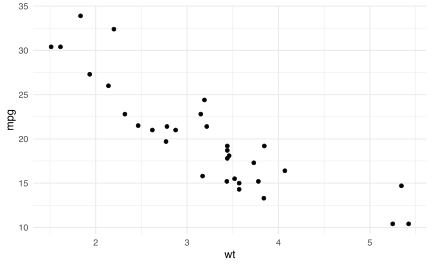
\includegraphics[width=0.7\linewidth]{Notas-Curso-Estadistica_files/figure-latex/unnamed-chunk-110-1} \end{center}

El objetivo es tratar la eficiencia del automóvil \texttt{mpg} con respecto a su peso \texttt{wt}.

Usaremos una regresión lineal para encontrar los coeficientes.

Primero hay que construir la matriz de diseño

\begin{Shaded}
\begin{Highlighting}[]
\NormalTok{X }\OtherTok{\textless{}{-}}\NormalTok{ mtcars}\SpecialCharTok{$}\NormalTok{wt}
\FunctionTok{head}\NormalTok{(X)}
\end{Highlighting}
\end{Shaded}

\begin{verbatim}
## [1] 2.620 2.875 2.320 3.215 3.440 3.460
\end{verbatim}

\begin{Shaded}
\begin{Highlighting}[]
\NormalTok{Y }\OtherTok{\textless{}{-}}\NormalTok{ mtcars}\SpecialCharTok{$}\NormalTok{mpg}
\FunctionTok{head}\NormalTok{(Y)}
\end{Highlighting}
\end{Shaded}

\begin{verbatim}
## [1] 21.0 21.0 22.8 21.4 18.7 18.1
\end{verbatim}

\begin{Shaded}
\begin{Highlighting}[]
\NormalTok{(beta1 }\OtherTok{\textless{}{-}} \FunctionTok{solve}\NormalTok{(}\FunctionTok{t}\NormalTok{(X) }\SpecialCharTok{\%*\%}\NormalTok{ X) }\SpecialCharTok{\%*\%} \FunctionTok{t}\NormalTok{(X) }\SpecialCharTok{\%*\%}\NormalTok{ Y)}
\end{Highlighting}
\end{Shaded}

\begin{verbatim}
##          [,1]
## [1,] 5.291624
\end{verbatim}

\begin{Shaded}
\begin{Highlighting}[]
\NormalTok{dfreg }\OtherTok{\textless{}{-}} \FunctionTok{data.frame}\NormalTok{(}\AttributeTok{x =}\NormalTok{ X, }\AttributeTok{yreg =}\NormalTok{ X }\SpecialCharTok{\%*\%}\NormalTok{ beta1) }\SpecialCharTok{\%\textgreater{}\%}
    \FunctionTok{arrange}\NormalTok{(x)}
\end{Highlighting}
\end{Shaded}

\begin{Shaded}
\begin{Highlighting}[]
\FunctionTok{ggplot}\NormalTok{(}\AttributeTok{data =} \FunctionTok{data.frame}\NormalTok{(}\AttributeTok{x =}\NormalTok{ X, }\AttributeTok{y =}\NormalTok{ Y)) }\SpecialCharTok{+} \FunctionTok{geom\_point}\NormalTok{(}\FunctionTok{aes}\NormalTok{(x,}
\NormalTok{    y)) }\SpecialCharTok{+} \FunctionTok{geom\_line}\NormalTok{(}\AttributeTok{data =}\NormalTok{ dfreg, }\FunctionTok{aes}\NormalTok{(x, yreg), }\AttributeTok{color =} \StringTok{"red"}\NormalTok{) }\SpecialCharTok{+}
    \FunctionTok{theme\_minimal}\NormalTok{()}
\end{Highlighting}
\end{Shaded}

\begin{center}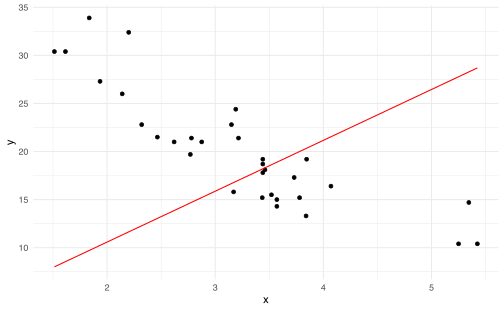
\includegraphics[width=0.7\linewidth]{Notas-Curso-Estadistica_files/figure-latex/unnamed-chunk-112-1} \end{center}

en donde podemos concluir que la relación lineal no modela de manera apropiada la relación observada en los datos. Por lo tanto es necesario incluir el intercepto \(\beta_0\) al modelo lineal:

\begin{Shaded}
\begin{Highlighting}[]
\NormalTok{X }\OtherTok{\textless{}{-}} \FunctionTok{cbind}\NormalTok{(}\DecValTok{1}\NormalTok{, mtcars}\SpecialCharTok{$}\NormalTok{wt)}
\FunctionTok{head}\NormalTok{(X)}
\end{Highlighting}
\end{Shaded}

\begin{verbatim}
##      [,1]  [,2]
## [1,]    1 2.620
## [2,]    1 2.875
## [3,]    1 2.320
## [4,]    1 3.215
## [5,]    1 3.440
## [6,]    1 3.460
\end{verbatim}

\begin{Shaded}
\begin{Highlighting}[]
\NormalTok{Y }\OtherTok{\textless{}{-}}\NormalTok{ mtcars}\SpecialCharTok{$}\NormalTok{mpg}
\FunctionTok{head}\NormalTok{(Y)}
\end{Highlighting}
\end{Shaded}

\begin{verbatim}
## [1] 21.0 21.0 22.8 21.4 18.7 18.1
\end{verbatim}

\begin{Shaded}
\begin{Highlighting}[]
\NormalTok{(beta01 }\OtherTok{\textless{}{-}} \FunctionTok{solve}\NormalTok{(}\FunctionTok{t}\NormalTok{(X) }\SpecialCharTok{\%*\%}\NormalTok{ X) }\SpecialCharTok{\%*\%} \FunctionTok{t}\NormalTok{(X) }\SpecialCharTok{\%*\%}\NormalTok{ Y)}
\end{Highlighting}
\end{Shaded}

\begin{verbatim}
##           [,1]
## [1,] 37.285126
## [2,] -5.344472
\end{verbatim}

\begin{Shaded}
\begin{Highlighting}[]
\NormalTok{dfreg }\OtherTok{\textless{}{-}} \FunctionTok{data.frame}\NormalTok{(}\AttributeTok{x =}\NormalTok{ X, }\AttributeTok{yreg =}\NormalTok{ X }\SpecialCharTok{\%*\%}\NormalTok{ beta01) }\SpecialCharTok{\%\textgreater{}\%}
    \FunctionTok{arrange}\NormalTok{(x}\FloatTok{.2}\NormalTok{)}
\end{Highlighting}
\end{Shaded}

\begin{Shaded}
\begin{Highlighting}[]
\FunctionTok{ggplot}\NormalTok{(}\AttributeTok{data =} \FunctionTok{data.frame}\NormalTok{(}\AttributeTok{x0 =}\NormalTok{ X[, }\DecValTok{1}\NormalTok{], }\AttributeTok{x1 =}\NormalTok{ X[, }\DecValTok{2}\NormalTok{],}
    \AttributeTok{y =}\NormalTok{ Y)) }\SpecialCharTok{+} \FunctionTok{geom\_point}\NormalTok{(}\FunctionTok{aes}\NormalTok{(x1, y)) }\SpecialCharTok{+} \FunctionTok{geom\_line}\NormalTok{(}\AttributeTok{data =}\NormalTok{ dfreg,}
    \FunctionTok{aes}\NormalTok{(x}\FloatTok{.2}\NormalTok{, yreg), }\AttributeTok{color =} \StringTok{"red"}\NormalTok{) }\SpecialCharTok{+} \FunctionTok{theme\_minimal}\NormalTok{()}
\end{Highlighting}
\end{Shaded}

\begin{center}\includegraphics[width=0.7\linewidth]{Notas-Curso-Estadistica_files/figure-latex/unnamed-chunk-114-1} \end{center}

El mismo resultado se puede obtener a través del comando \verb|lm|:

\begin{Shaded}
\begin{Highlighting}[]
\FunctionTok{lm}\NormalTok{(mpg }\SpecialCharTok{\textasciitilde{}} \SpecialCharTok{{-}}\DecValTok{1} \SpecialCharTok{+}\NormalTok{ wt, }\AttributeTok{data =}\NormalTok{ mtcars)}
\end{Highlighting}
\end{Shaded}

\begin{verbatim}
## 
## Call:
## lm(formula = mpg ~ -1 + wt, data = mtcars)
## 
## Coefficients:
##    wt  
## 5.292
\end{verbatim}

\begin{Shaded}
\begin{Highlighting}[]
\FunctionTok{lm}\NormalTok{(mpg }\SpecialCharTok{\textasciitilde{}}\NormalTok{ wt, }\AttributeTok{data =}\NormalTok{ mtcars)}
\end{Highlighting}
\end{Shaded}

\begin{verbatim}
## 
## Call:
## lm(formula = mpg ~ wt, data = mtcars)
## 
## Coefficients:
## (Intercept)           wt  
##      37.285       -5.344
\end{verbatim}

Suponga que queremos trabajar con la variable categorica \texttt{cyl} (Número de cilindros) como única covariable. Lo que se debe hacer es codificar la variable categórica:

\begin{Shaded}
\begin{Highlighting}[]
\NormalTok{X }\OtherTok{\textless{}{-}} \FunctionTok{model.matrix}\NormalTok{(mpg }\SpecialCharTok{\textasciitilde{}}\NormalTok{ cyl, }\AttributeTok{data =}\NormalTok{ mtcars)}

\FunctionTok{head}\NormalTok{(X)}
\end{Highlighting}
\end{Shaded}

\begin{verbatim}
##                   (Intercept) cyl6 cyl8
## Mazda RX4                   1    1    0
## Mazda RX4 Wag               1    1    0
## Datsun 710                  1    0    0
## Hornet 4 Drive              1    1    0
## Hornet Sportabout           1    0    1
## Valiant                     1    1    0
\end{verbatim}

\begin{Shaded}
\begin{Highlighting}[]
\NormalTok{(betas }\OtherTok{\textless{}{-}} \FunctionTok{solve}\NormalTok{(}\FunctionTok{t}\NormalTok{(X) }\SpecialCharTok{\%*\%}\NormalTok{ X) }\SpecialCharTok{\%*\%} \FunctionTok{t}\NormalTok{(X) }\SpecialCharTok{\%*\%}\NormalTok{ Y)}
\end{Highlighting}
\end{Shaded}

\begin{verbatim}
##                   [,1]
## (Intercept)  26.663636
## cyl6         -6.920779
## cyl8        -11.563636
\end{verbatim}

\begin{Shaded}
\begin{Highlighting}[]
\NormalTok{(cylreg }\OtherTok{\textless{}{-}} \FunctionTok{lm}\NormalTok{(mpg }\SpecialCharTok{\textasciitilde{}}\NormalTok{ cyl, }\AttributeTok{data =}\NormalTok{ mtcars))}
\end{Highlighting}
\end{Shaded}

\begin{verbatim}
## 
## Call:
## lm(formula = mpg ~ cyl, data = mtcars)
## 
## Coefficients:
## (Intercept)         cyl6         cyl8  
##      26.664       -6.921      -11.564
\end{verbatim}

\begin{Shaded}
\begin{Highlighting}[]
\NormalTok{(betaslm }\OtherTok{\textless{}{-}} \FunctionTok{coefficients}\NormalTok{(cylreg))}
\end{Highlighting}
\end{Shaded}

\begin{verbatim}
## (Intercept)        cyl6        cyl8 
##   26.663636   -6.920779  -11.563636
\end{verbatim}

\begin{Shaded}
\begin{Highlighting}[]
\CommentTok{\# Efecto cyl4: cyl4 = 1, cyl6 = 0, cyl8 = 0}

\NormalTok{betaslm[}\DecValTok{1}\NormalTok{]}
\end{Highlighting}
\end{Shaded}

\begin{verbatim}
## (Intercept) 
##    26.66364
\end{verbatim}

\begin{Shaded}
\begin{Highlighting}[]
\CommentTok{\# Efecto cyl6: cyl4 = 1, cyl6 = 1, cyl8 = 0}

\NormalTok{betaslm[}\DecValTok{1}\NormalTok{] }\SpecialCharTok{+}\NormalTok{ betaslm[}\DecValTok{2}\NormalTok{]}
\end{Highlighting}
\end{Shaded}

\begin{verbatim}
## (Intercept) 
##    19.74286
\end{verbatim}

\begin{Shaded}
\begin{Highlighting}[]
\CommentTok{\# Efecto cyl8: cyl4 = 1, cyl6 = 0, cyl8 = 1}

\NormalTok{betaslm[}\DecValTok{1}\NormalTok{] }\SpecialCharTok{+}\NormalTok{ betaslm[}\DecValTok{3}\NormalTok{]}
\end{Highlighting}
\end{Shaded}

\begin{verbatim}
## (Intercept) 
##        15.1
\end{verbatim}

\hypertarget{propiedades-estaduxedsticas-3}{%
\section{Propiedades estadísticas}\label{propiedades-estaduxedsticas-3}}

Hasta ahora se han hecho pocos supuestos acerca de la distribución de los datos. Si asumimos que las observaciones \(Y_i\) son no correlacionadas y que tienen varianza constante \(\sigma^2\) y además las covariables son fijas (no aleatorias), entonces:

\begin{align*}
E[\hat \beta]&=(\boldsymbol{X}^{\top} \boldsymbol{X})^{-1} \boldsymbol{X}^{\top}E[\boldsymbol{Y}] \\ 
&=(\boldsymbol{X}^{\top} \boldsymbol{X})^{-1} \boldsymbol{X}^{\top}\boldsymbol{X}\beta\\
&=\beta \\
\text{Var}[\hat \beta] &= (\boldsymbol{X}^{\top} \boldsymbol{X})^{-1} \boldsymbol{X}^{\top}\text{Var}[\boldsymbol{Y}] ((\boldsymbol{X}^{\top} \boldsymbol{X})^{-1} \boldsymbol{X}^{\top})^{\top} \\
& = \sigma^2 (\boldsymbol{X}^{\top} \boldsymbol{X})^{-1}
\end{align*}

Note que \(\sigma^{2}\) puede ser estimado a través de:

\begin{align*}
 \hat{\sigma}^{2} 
 &=  \frac{1}{n-p-1} \sum_{i=1}^{n} \left( Y_{i} - \hat{Y}_{i}\right)^{2} \\
 &= \frac{1}{n-p-1}\left\Vert Y - X\hat{\beta} \right\Vert^{2} \\
 &=   \frac{1}{n-p-1} \left\Vert Y-\operatorname{Proy}_{V}Y \right\Vert^{2} 
 \end{align*}

Otra forma de verlo es
\begin{align*}
Y-\operatorname{Proy}_{V}Y  
&= X\beta + \varepsilon -  \operatorname{Proy}_{V}( X\beta + \varepsilon) \\
&= X\beta - \operatorname{Proy}_{V}( \underbrace{X\beta}_{\in V}) + \varepsilon - \underbrace{\operatorname{Proy}_{V}( \varepsilon)}_{=0} \\
&= X\beta -X\beta + \varepsilon \\
&=  \operatorname{Proy}_{V^{\top}}( \varepsilon)
 \end{align*}

\begin{equation*}
\hat{\sigma}^{2} 
= \frac{1}{\operatorname{dim}(V^{\top})}\left\Vert \operatorname{Proy}_{V^{\top}}\varepsilon\right\Vert \\
\end{equation*}

Cumple con la propiedad que \(\mathbb{E}\left[\hat{\sigma}^{2}\right] = \sigma^{2}\) (estimador insesgado).

Para poder hacer inferencia sobre \(\beta\) y \(\sigma^2\) se puede asumir además que los errores son gaussianos:

\begin{equation*}
\varepsilon\sim \mathcal{N}\left(0,\sigma^{2}I\right).
\end{equation*}

y de esta forma se obtiene:

\begin{equation*}
Y = X\beta + \varepsilon \sim \mathcal{N}\left(X\beta,\sigma^{2}I\right)
\end{equation*}

Y además:

\begin{align*}
\hat{\beta} \sim  \mathcal{N}\left(\beta,\sigma^2 (X^{\top}X)^{-1}\right) 
\end{align*}

Por otro lado se puede comprobar que:
\[(n-p-1)\hat{\sigma}^{2} \sim \sigma^{2} \chi^{2}_{n-p-1}.\]
y además se puede comprobar que \(\hat \beta\) y \(\hat \sigma^2\) son independientes.

\begin{exercise}
\protect\hypertarget{exr:unnamed-chunk-118}{}\label{exr:unnamed-chunk-118}Encuentre la varianza para \(\hat \beta_{0}\) y \(\hat \beta_{1}\) para el caso de la regresión simple.
\end{exercise}

\hypertarget{prueba-t}{%
\subsection{\texorpdfstring{Prueba \(t\)}{Prueba t}}\label{prueba-t}}

La significancia de los parámetros \(\beta_j\) se puede verificar a través de la siguiente prueba de hipótesis:

\begin{equation*}
 H_{0}: \beta_{j} = 0 \quad \text{ vs } \quad H_{1}:\beta_{j}\neq 0.
 \end{equation*}

En donde el estadístico de prueba es:

\begin{equation*}
 z_{j} = \frac{\hat{\beta}_{j}}{\hat{\sigma} \sqrt{v_{j}}} 
 \end{equation*}

donde \(v_{j}\) es el \(j\)-esimo elemento de la diagonal de \((X^{\top}X)^{-1}\).

Bajo \(H_{0}\): \(z_{j} \sim t_{n-p-1}\) y se rechaza \(H_{0}\) al nivel \(\alpha\) si:

\begin{equation*}
 \left\vert z_{j} \right\vert > t_{n-p-1, 1-\frac{\alpha}{2}} 
 \end{equation*}

\hypertarget{prueba-f}{%
\subsection{\texorpdfstring{Prueba \(F\)}{Prueba F}}\label{prueba-f}}

Si uno busca medir la significancia de todos los parámetros \(\beta_j\) de forma simultánea, excepto el intercepto. En este caso podemos definir la siguiente hipótesis nula:
\begin{equation*}
 H_{0}: \beta_{1} = \cdots =\beta_{p} = 0 \quad 
 \text{  vs   }\quad H_{1}: \text{ al menos un \(\beta\) no es cero}.
 \end{equation*}

Lo cual es equivalente a comparar el modelo nulo \(Y=\beta_{0}+\varepsilon\) contra el modelo completo \(Y=\beta_{0}+ \beta_{1}X_{1} + \cdots + \beta_{p}X_{p} + \varepsilon\).

Defina la suma total de cuadrados (\(TSS\)) y la suma de residuos al cuadrado (\(RSS\)) como:
\begin{align*}
 TSS &= \sum_{i=1}^{n} \left( Y_{i} -\overline{Y} \right)^{2} \\
 RSS &= \sum_{i=1}^{n} \left( Y_{i} -\hat{Y_i} \right)^{2} \\
 \end{align*}

Entonces el estadístico de prueba es:

\begin{equation*}
 F = \frac{\frac{TSS-RSS}{p}}{\frac{RSS}{n-p-1}} \stackrel{H_0}{\sim} \frac{\chi^{2}_{p}}{\chi^{2}_{n-p-1}}.
 \end{equation*}

y rechazaríamos \(H_{0}\) al nivel \(\alpha\) si:

\begin{equation*}
 F > F_{p, n-p-1, 1-\alpha}.
 \end{equation*}

Si por otro lado queremos probar que un conjunto de \(q\) covariables son no-significativas entonces probamos (sin pérdida de generalidad):
\begin{align*}
H_0: \beta_{p-q+1}=\beta_{p-q+2}=\cdots=\beta_p=0
\end{align*}

a través de la comparación de un modelo completo y uno reducido:
\begin{align*}
Y&=\beta_{0}+ \beta_{1}X_{1} + \cdots + \beta_{p}X_{p} + \varepsilon \qquad \text{Modelo completo} \\
Y&=\beta_{0}+ \beta_{1}X_{1} + \cdots + \beta_{p-q}X_{p-q} + \varepsilon \qquad \text{Modelo reducido}
\end{align*}

usando el estadístico de prueba:

\begin{equation*}
 F = \frac{\frac{RSS_0-RSS}{q}}{\frac{RSS}{n-p-1}} \stackrel{H_0}{\sim} \frac{\chi^{2}_{q}}{\chi^{2}_{n-p-1}}.
 \end{equation*}

donde \(RSS_0\) es la suma de residuos al cuadrado del modelo reducido. En este caso se rechazaría \(H_0\) al nivel \(\alpha\) si \(F>F_{q, n-p-1, 1-\alpha}\).

\hypertarget{laboratorio-2}{%
\subsection{Laboratorio}\label{laboratorio-2}}

Siguiendo con nuestro ejemplo, vamos a explorar un poco más la función \texttt{lm}.

\begin{Shaded}
\begin{Highlighting}[]
\NormalTok{modelo\_wt }\OtherTok{\textless{}{-}} \FunctionTok{lm}\NormalTok{(mpg }\SpecialCharTok{\textasciitilde{}}\NormalTok{ wt, }\AttributeTok{data =}\NormalTok{ mtcars)}
\FunctionTok{summary}\NormalTok{(modelo\_wt)}
\end{Highlighting}
\end{Shaded}

\begin{verbatim}
## 
## Call:
## lm(formula = mpg ~ wt, data = mtcars)
## 
## Residuals:
##     Min      1Q  Median      3Q     Max 
## -4.5432 -2.3647 -0.1252  1.4096  6.8727 
## 
## Coefficients:
##             Estimate Std. Error t value Pr(>|t|)    
## (Intercept)  37.2851     1.8776  19.858  < 2e-16 ***
## wt           -5.3445     0.5591  -9.559 1.29e-10 ***
## ---
## Signif. codes:  0 '***' 0.001 '**' 0.01 '*' 0.05 '.' 0.1 ' ' 1
## 
## Residual standard error: 3.046 on 30 degrees of freedom
## Multiple R-squared:  0.7528, Adjusted R-squared:  0.7446 
## F-statistic: 91.38 on 1 and 30 DF,  p-value: 1.294e-10
\end{verbatim}

\begin{Shaded}
\begin{Highlighting}[]
\NormalTok{modelo\_wt\_cyl }\OtherTok{\textless{}{-}} \FunctionTok{lm}\NormalTok{(mpg }\SpecialCharTok{\textasciitilde{}}\NormalTok{ wt }\SpecialCharTok{+}\NormalTok{ cyl, }\AttributeTok{data =}\NormalTok{ mtcars)}
\FunctionTok{summary}\NormalTok{(modelo\_wt\_cyl)}
\end{Highlighting}
\end{Shaded}

\begin{verbatim}
## 
## Call:
## lm(formula = mpg ~ wt + cyl, data = mtcars)
## 
## Residuals:
##     Min      1Q  Median      3Q     Max 
## -4.5890 -1.2357 -0.5159  1.3845  5.7915 
## 
## Coefficients:
##             Estimate Std. Error t value Pr(>|t|)    
## (Intercept)  33.9908     1.8878  18.006  < 2e-16 ***
## wt           -3.2056     0.7539  -4.252 0.000213 ***
## cyl6         -4.2556     1.3861  -3.070 0.004718 ** 
## cyl8         -6.0709     1.6523  -3.674 0.000999 ***
## ---
## Signif. codes:  0 '***' 0.001 '**' 0.01 '*' 0.05 '.' 0.1 ' ' 1
## 
## Residual standard error: 2.557 on 28 degrees of freedom
## Multiple R-squared:  0.8374, Adjusted R-squared:   0.82 
## F-statistic: 48.08 on 3 and 28 DF,  p-value: 3.594e-11
\end{verbatim}

\begin{Shaded}
\begin{Highlighting}[]
\FunctionTok{anova}\NormalTok{(modelo\_wt, modelo\_wt\_cyl)}
\end{Highlighting}
\end{Shaded}

\begin{verbatim}
## Analysis of Variance Table
## 
## Model 1: mpg ~ wt
## Model 2: mpg ~ wt + cyl
##   Res.Df    RSS Df Sum of Sq      F   Pr(>F)   
## 1     30 278.32                                
## 2     28 183.06  2    95.263 7.2856 0.002835 **
## ---
## Signif. codes:  0 '***' 0.001 '**' 0.01 '*' 0.05 '.' 0.1 ' ' 1
\end{verbatim}

\begin{Shaded}
\begin{Highlighting}[]
\NormalTok{modelo\_nulo }\OtherTok{\textless{}{-}} \FunctionTok{lm}\NormalTok{(mpg }\SpecialCharTok{\textasciitilde{}} \DecValTok{1}\NormalTok{, }\AttributeTok{data =}\NormalTok{ mtcars)}
\FunctionTok{summary}\NormalTok{(modelo\_nulo)}
\end{Highlighting}
\end{Shaded}

\begin{verbatim}
## 
## Call:
## lm(formula = mpg ~ 1, data = mtcars)
## 
## Residuals:
##     Min      1Q  Median      3Q     Max 
## -9.6906 -4.6656 -0.8906  2.7094 13.8094 
## 
## Coefficients:
##             Estimate Std. Error t value Pr(>|t|)    
## (Intercept)   20.091      1.065   18.86   <2e-16 ***
## ---
## Signif. codes:  0 '***' 0.001 '**' 0.01 '*' 0.05 '.' 0.1 ' ' 1
## 
## Residual standard error: 6.027 on 31 degrees of freedom
\end{verbatim}

\begin{Shaded}
\begin{Highlighting}[]
\FunctionTok{anova}\NormalTok{(modelo\_nulo, modelo\_wt\_cyl)}
\end{Highlighting}
\end{Shaded}

\begin{verbatim}
## Analysis of Variance Table
## 
## Model 1: mpg ~ 1
## Model 2: mpg ~ wt + cyl
##   Res.Df     RSS Df Sum of Sq      F    Pr(>F)    
## 1     31 1126.05                                  
## 2     28  183.06  3    942.99 48.079 3.594e-11 ***
## ---
## Signif. codes:  0 '***' 0.001 '**' 0.01 '*' 0.05 '.' 0.1 ' ' 1
\end{verbatim}

\begin{Shaded}
\begin{Highlighting}[]
\NormalTok{fit }\OtherTok{\textless{}{-}} \FunctionTok{lm}\NormalTok{(mpg }\SpecialCharTok{\textasciitilde{}}\NormalTok{ ., }\AttributeTok{data =}\NormalTok{ mtcars)}
\FunctionTok{summary}\NormalTok{(fit)}
\end{Highlighting}
\end{Shaded}

\begin{verbatim}
## 
## Call:
## lm(formula = mpg ~ ., data = mtcars)
## 
## Residuals:
##     Min      1Q  Median      3Q     Max 
## -3.5087 -1.3584 -0.0948  0.7745  4.6251 
## 
## Coefficients:
##                 Estimate Std. Error t value Pr(>|t|)  
## (Intercept)     23.87913   20.06582   1.190   0.2525  
## cyl6            -2.64870    3.04089  -0.871   0.3975  
## cyl8            -0.33616    7.15954  -0.047   0.9632  
## disp             0.03555    0.03190   1.114   0.2827  
## hp              -0.07051    0.03943  -1.788   0.0939 .
## drat             1.18283    2.48348   0.476   0.6407  
## wt              -4.52978    2.53875  -1.784   0.0946 .
## qsec             0.36784    0.93540   0.393   0.6997  
## vsStraight-Line  1.93085    2.87126   0.672   0.5115  
## ammanual         1.21212    3.21355   0.377   0.7113  
## gear4            1.11435    3.79952   0.293   0.7733  
## gear5            2.52840    3.73636   0.677   0.5089  
## carb2           -0.97935    2.31797  -0.423   0.6787  
## carb3            2.99964    4.29355   0.699   0.4955  
## carb4            1.09142    4.44962   0.245   0.8096  
## carb6            4.47757    6.38406   0.701   0.4938  
## carb8            7.25041    8.36057   0.867   0.3995  
## ---
## Signif. codes:  0 '***' 0.001 '**' 0.01 '*' 0.05 '.' 0.1 ' ' 1
## 
## Residual standard error: 2.833 on 15 degrees of freedom
## Multiple R-squared:  0.8931, Adjusted R-squared:  0.779 
## F-statistic:  7.83 on 16 and 15 DF,  p-value: 0.000124
\end{verbatim}

\hypertarget{medida-de-bondad-de-ajuste}{%
\section{Medida de bondad de ajuste}\label{medida-de-bondad-de-ajuste}}

A través de la prueba \(F\) uno puede concluir si un modelo es significativo o no bajo un cierto nivel de confianza, o bien puede comparar si un modelo reducido es más significativo que uno completo, pero no nos da herramientas para decidir si un modelo es mejor que otro.

Hay varias medidas para comparar modelos (la veremos con más detalle en otro capítulo):

\begin{itemize}
\tightlist
\item
  Error estándar residual (\(\sigma\))
\item
  \(R^{2}\) y \(R^{2}\) ajustado
\item
  \(C_{p}\) de Mallows
\item
  Akaike Information Criterion (AIC)
\item
  Bayesian Information Criterion (BIC)
\end{itemize}

Los índices \(C_{p}\) de Mallows, AIC y BIC los veremos después.

\begin{description}
\tightlist
\item[Error estándar residual]
Se define como
\end{description}

\begin{align*}
\mathrm{RSE} 
&=  \sqrt{\hat{\sigma^{2}}}\\
&= \sqrt{\frac{1}{n-p-1} \sum_{i=1}^{n} \left( Y_{i} - \hat{Y}_{i}\right)^{2}} \\
&= \sqrt{\frac{\mathrm{RSS}}{n-p-1}}
\end{align*}

Entre más pequeño mejor, pero \textbf{depende de las unidades de \(Y\)}.

\begin{description}
\tightlist
\item[Estadístico \(R^{2}\)]
\begin{equation*}
R^{2} = \frac{\mathrm{TSS}-\mathrm{RSS}}{\mathrm{TSS}} = 1-\frac{\mathrm{RSS}}{\mathrm{TSS}}
\end{equation*}
\end{description}

\begin{itemize}
\tightlist
\item
  \textbf{RSS:} Varianza sin explicar por el modelo \textbf{completo}.
\item
  \textbf{TSS:} Varianza sin explicar por el modelo \textbf{nulo}.
\end{itemize}

Interpretación: proporción de variabilidad en \(Y\) que es explicada a través de las covariables en \(X\). Ya que \(TSS-RSS\) representa la variabilidad explicada a través del modelo de regresión.

Limitación: puede tener un valor alto bajo un número grande de covariables, ya que \(RSS\) tiende a ser bajo conforme aumenta la complejidad del modelo (sobreajuste).

\begin{description}
\tightlist
\item[Estadístico \(R^{2}\) ajustado]
\begin{equation*}
R^{2}_{adj} = 1-\frac{\frac{\mathrm{RSS}}{n-p-1}}{\frac{\mathrm{TSS}}{n-1}}
\end{equation*}
\end{description}

\hypertarget{laboratorio-3}{%
\subsection{Laboratorio}\label{laboratorio-3}}

\begin{Shaded}
\begin{Highlighting}[]
\CommentTok{\# Número de datos}
\NormalTok{n }\OtherTok{\textless{}{-}} \DecValTok{1000}
\CommentTok{\# Número de variables}
\NormalTok{p }\OtherTok{\textless{}{-}} \DecValTok{2}

\NormalTok{x1 }\OtherTok{\textless{}{-}} \FunctionTok{rnorm}\NormalTok{(}\DecValTok{1000}\NormalTok{)}
\NormalTok{x2 }\OtherTok{\textless{}{-}} \FunctionTok{runif}\NormalTok{(}\DecValTok{1000}\NormalTok{)}
\NormalTok{y }\OtherTok{\textless{}{-}} \DecValTok{1} \SpecialCharTok{+}\NormalTok{ x1 }\SpecialCharTok{+}\NormalTok{ x2 }\SpecialCharTok{+} \FunctionTok{rnorm}\NormalTok{(}\DecValTok{1000}\NormalTok{, }\AttributeTok{sd =} \FloatTok{0.5}\NormalTok{)}

\NormalTok{fit }\OtherTok{\textless{}{-}} \FunctionTok{lm}\NormalTok{(y }\SpecialCharTok{\textasciitilde{}}\NormalTok{ x1 }\SpecialCharTok{+}\NormalTok{ x2)}
\end{Highlighting}
\end{Shaded}

\hypertarget{r2}{%
\subsubsection{\texorpdfstring{\(R^2\)}{R\^{}2}}\label{r2}}

\begin{Shaded}
\begin{Highlighting}[]
\NormalTok{(TSS }\OtherTok{\textless{}{-}} \FunctionTok{sum}\NormalTok{((y }\SpecialCharTok{{-}} \FunctionTok{mean}\NormalTok{(y))}\SpecialCharTok{\^{}}\DecValTok{2}\NormalTok{))}
\end{Highlighting}
\end{Shaded}

\begin{verbatim}
## [1] 1404.421
\end{verbatim}

\begin{Shaded}
\begin{Highlighting}[]
\NormalTok{(RSS }\OtherTok{\textless{}{-}} \FunctionTok{sum}\NormalTok{((y }\SpecialCharTok{{-}} \FunctionTok{fitted}\NormalTok{(fit))}\SpecialCharTok{\^{}}\DecValTok{2}\NormalTok{))}
\end{Highlighting}
\end{Shaded}

\begin{verbatim}
## [1] 256.8679
\end{verbatim}

\begin{Shaded}
\begin{Highlighting}[]
\DecValTok{1} \SpecialCharTok{{-}}\NormalTok{ RSS}\SpecialCharTok{/}\NormalTok{TSS}
\end{Highlighting}
\end{Shaded}

\begin{verbatim}
## [1] 0.8171005
\end{verbatim}

Otra forma de entender el \(R^2\) es notando que

\begin{Shaded}
\begin{Highlighting}[]
\FunctionTok{cor}\NormalTok{(y, }\FunctionTok{fitted}\NormalTok{(fit))}\SpecialCharTok{\^{}}\DecValTok{2}
\end{Highlighting}
\end{Shaded}

\begin{verbatim}
## [1] 0.8171005
\end{verbatim}

\hypertarget{r2-ajustado}{%
\subsubsection{\texorpdfstring{\(R^2\) ajustado}{R\^{}2 ajustado}}\label{r2-ajustado}}

\begin{Shaded}
\begin{Highlighting}[]
\NormalTok{(TSS\_adj }\OtherTok{\textless{}{-}}\NormalTok{ TSS}\SpecialCharTok{/}\NormalTok{(n }\SpecialCharTok{{-}} \DecValTok{1}\NormalTok{))}
\end{Highlighting}
\end{Shaded}

\begin{verbatim}
## [1] 1.405827
\end{verbatim}

\begin{Shaded}
\begin{Highlighting}[]
\NormalTok{(RSS\_adj }\OtherTok{\textless{}{-}}\NormalTok{ RSS}\SpecialCharTok{/}\NormalTok{(n }\SpecialCharTok{{-}}\NormalTok{ p }\SpecialCharTok{{-}} \DecValTok{1}\NormalTok{))}
\end{Highlighting}
\end{Shaded}

\begin{verbatim}
## [1] 0.2576408
\end{verbatim}

\begin{Shaded}
\begin{Highlighting}[]
\DecValTok{1} \SpecialCharTok{{-}}\NormalTok{ RSS\_adj}\SpecialCharTok{/}\NormalTok{TSS\_adj}
\end{Highlighting}
\end{Shaded}

\begin{verbatim}
## [1] 0.8167336
\end{verbatim}

\hypertarget{summary}{%
\subsubsection{\texorpdfstring{\texttt{summary}}{summary}}\label{summary}}

\begin{Shaded}
\begin{Highlighting}[]
\FunctionTok{summary}\NormalTok{(fit)}
\end{Highlighting}
\end{Shaded}

\begin{verbatim}
## 
## Call:
## lm(formula = y ~ x1 + x2)
## 
## Residuals:
##      Min       1Q   Median       3Q      Max 
## -1.73583 -0.35052  0.01175  0.33270  1.42618 
## 
## Coefficients:
##             Estimate Std. Error t value Pr(>|t|)    
## (Intercept)  1.05443    0.03252   32.42   <2e-16 ***
## x1           1.02131    0.01573   64.92   <2e-16 ***
## x2           0.91189    0.05655   16.13   <2e-16 ***
## ---
## Signif. codes:  0 '***' 0.001 '**' 0.01 '*' 0.05 '.' 0.1 ' ' 1
## 
## Residual standard error: 0.5076 on 997 degrees of freedom
## Multiple R-squared:  0.8171, Adjusted R-squared:  0.8167 
## F-statistic:  2227 on 2 and 997 DF,  p-value: < 2.2e-16
\end{verbatim}

\hypertarget{predicciuxf3n}{%
\section{Predicción}\label{predicciuxf3n}}

Hay dos tipos de errores que se deben considerar en regresiones lineales:

\begin{enumerate}
\def\labelenumi{\arabic{enumi}.}
\tightlist
\item
  \textbf{Error Reducible:} Recuerde que \(\hat{Y} = X\hat{\beta}\) es el estimador de la función \(f(X)=X\beta = \beta_{0} + \beta_{1}X_{1}+\cdots+\beta_{p}X_{p}\).
\end{enumerate}

Por lo tanto su error (reducible) es:

\begin{equation*}
\left(  f(X) - \hat{Y}\right) ^{2}. 
\end{equation*}

Para un conjunto de datos \(X_{0}\), tenemos que

\begin{align*}
 & \hat{\beta} \sim  \mathcal{N}\left(\beta, \sigma^{2}\left( (X_{0}^{\top}X_{0})^{-1} \right)\right) \\
 \implies & \hat{Y} = X_{0}\hat{\beta} \sim \mathcal{N}\left((X_{0}\beta,\sigma^{2}X_{0}^{\top}((X_{0}^{\top}X_{0})^{-1}X_{0})) \right)
\end{align*}

Por lo tanto un \textbf{intervalo de confianza} al \(1-\alpha\) para \(X_0\beta\) es

\begin{equation*}
X_{0}\hat \beta \pm z_{1-\frac{\alpha}{2}} \hat{\sigma} \sqrt{X_{0}^{\top}(X_{0}^{\top}X_{0})^{-1}X_{0}}.
\end{equation*}

\begin{enumerate}
\def\labelenumi{\arabic{enumi}.}
\setcounter{enumi}{1}
\tightlist
\item
  \textbf{Error irreducible:} Aún conociendo perfectamente los \(\beta\)'s, existe el error desconocido \(\varepsilon\sim \mathcal{N}\left(0,\sigma^{2}\right)\) del modelo
\end{enumerate}

\begin{equation*}
Y = X\beta + \varepsilon.
\end{equation*}

Entonces la varianza total de la predicción sería

\begin{equation*}
\sigma^{2} +  \sigma^{2}X_{0}^{\top}((X_{0}^{\top}X_{0})^{-1}X_{0}) 
\end{equation*}

Entonces un \textbf{intervalo de predicción} al \(1-\alpha\) debe tomar en cuenta ese error y por lo tanto

\begin{equation*}
X_{0}\beta \pm z_{1-\frac{\alpha}{2}} \hat{\sigma} \sqrt{1+X_{0}^{\top}(X_{0}^{\top}X_{0})^{-1}X_{0}}.
\end{equation*}

\hypertarget{laboratorio-4}{%
\subsection{Laboratorio}\label{laboratorio-4}}

\begin{Shaded}
\begin{Highlighting}[]
\NormalTok{lm.r }\OtherTok{\textless{}{-}} \FunctionTok{lm}\NormalTok{(mpg }\SpecialCharTok{\textasciitilde{}}\NormalTok{ wt, }\AttributeTok{data =}\NormalTok{ mtcars)}

\FunctionTok{range}\NormalTok{(mtcars}\SpecialCharTok{$}\NormalTok{wt)}
\end{Highlighting}
\end{Shaded}

\begin{verbatim}
## [1] 1.513 5.424
\end{verbatim}

\begin{Shaded}
\begin{Highlighting}[]
\NormalTok{(datos\_nuevos }\OtherTok{\textless{}{-}} \FunctionTok{data.frame}\NormalTok{(}\AttributeTok{wt =} \FunctionTok{c}\NormalTok{(}\FloatTok{2.5}\NormalTok{, }\DecValTok{3}\NormalTok{, }\FloatTok{3.5}\NormalTok{)))}
\end{Highlighting}
\end{Shaded}

\begin{verbatim}
##    wt
## 1 2.5
## 2 3.0
## 3 3.5
\end{verbatim}

\begin{Shaded}
\begin{Highlighting}[]
\FunctionTok{predict}\NormalTok{(}\AttributeTok{object =}\NormalTok{ lm.r, }\AttributeTok{newdata =}\NormalTok{ datos\_nuevos, }\AttributeTok{interval =} \StringTok{"confidence"}\NormalTok{)}
\end{Highlighting}
\end{Shaded}

\begin{verbatim}
##        fit      lwr      upr
## 1 23.92395 22.55284 25.29506
## 2 21.25171 20.12444 22.37899
## 3 18.57948 17.43342 19.72553
\end{verbatim}

\begin{Shaded}
\begin{Highlighting}[]
\FunctionTok{predict}\NormalTok{(}\AttributeTok{object =}\NormalTok{ lm.r, }\AttributeTok{newdata =}\NormalTok{ datos\_nuevos, }\AttributeTok{interval =} \StringTok{"prediction"}\NormalTok{)}
\end{Highlighting}
\end{Shaded}

\begin{verbatim}
##        fit      lwr      upr
## 1 23.92395 17.55411 30.29378
## 2 21.25171 14.92987 27.57355
## 3 18.57948 12.25426 24.90469
\end{verbatim}

\hypertarget{ajuste-de-la-regresiuxf3n-sin-intervalos-de-confianza}{%
\subsubsection{Ajuste de la regresión sin intervalos de confianza}\label{ajuste-de-la-regresiuxf3n-sin-intervalos-de-confianza}}

\begin{Shaded}
\begin{Highlighting}[]
\NormalTok{p }\OtherTok{\textless{}{-}} \FunctionTok{ggplot}\NormalTok{(mtcars, }\FunctionTok{aes}\NormalTok{(}\AttributeTok{x =}\NormalTok{ wt, }\AttributeTok{y =}\NormalTok{ mpg)) }
\NormalTok{p }\OtherTok{\textless{}{-}}\NormalTok{ p }\SpecialCharTok{+} \FunctionTok{geom\_point}\NormalTok{(}\AttributeTok{size =} \DecValTok{2}\NormalTok{)       }\CommentTok{\# Use circulos de tamaño 2}
\NormalTok{p }\OtherTok{\textless{}{-}}\NormalTok{ p }\SpecialCharTok{+} \FunctionTok{geom\_smooth}\NormalTok{(}\AttributeTok{method =}\NormalTok{ lm,   }\CommentTok{\# Agregar la línea de regresión }
              \AttributeTok{se =} \ConstantTok{FALSE}\NormalTok{,           }\CommentTok{\# NO incluir el intervalo de confianza   }
              \AttributeTok{size =} \DecValTok{1}\NormalTok{,}
              \AttributeTok{col =} \StringTok{"red"}\NormalTok{)          }\CommentTok{\# Línea de color rojo }
\NormalTok{p }\OtherTok{\textless{}{-}}\NormalTok{ p }\SpecialCharTok{+} \FunctionTok{theme\_bw}\NormalTok{()                 }\CommentTok{\# Tema de fondo blanco}
\NormalTok{p }\OtherTok{\textless{}{-}}\NormalTok{ p }\SpecialCharTok{+} \FunctionTok{theme}\NormalTok{(}\AttributeTok{axis.text =} \FunctionTok{element\_text}\NormalTok{(}\AttributeTok{size =} \DecValTok{20}\NormalTok{),  }\CommentTok{\# Aumentar el tamaño }
               \AttributeTok{axis.title =} \FunctionTok{element\_text}\NormalTok{(}\AttributeTok{size =} \DecValTok{20}\NormalTok{)) }\CommentTok{\# de letra en los ejes}

\CommentTok{\# Dibujar el gráfico}
\NormalTok{p   }
\end{Highlighting}
\end{Shaded}

\begin{center}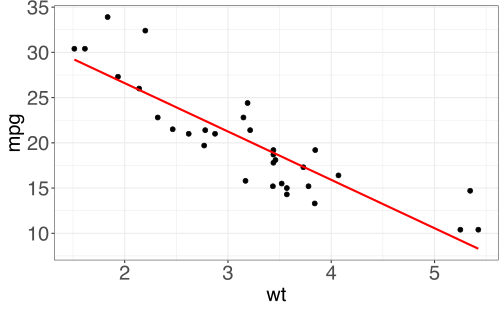
\includegraphics[width=0.7\linewidth]{Notas-Curso-Estadistica_files/figure-latex/unnamed-chunk-126-1} \end{center}

\begin{Shaded}
\begin{Highlighting}[]
\CommentTok{\# \# Guardar el gráfico en un archivo pdf}
\CommentTok{\# ggsave(filename = \textquotesingle{}linear\_reg\_sin\_IC.pdf\textquotesingle{}) \# }
\end{Highlighting}
\end{Shaded}

\hypertarget{ajuste-de-la-regresiuxf3n-con-intervalos-de-confianza}{%
\subsubsection{Ajuste de la regresión con intervalos de confianza}\label{ajuste-de-la-regresiuxf3n-con-intervalos-de-confianza}}

\begin{Shaded}
\begin{Highlighting}[]
\NormalTok{p }\OtherTok{\textless{}{-}} \FunctionTok{ggplot}\NormalTok{(mtcars, }\FunctionTok{aes}\NormalTok{(}\AttributeTok{x =}\NormalTok{ wt, }\AttributeTok{y =}\NormalTok{ mpg)) }
\NormalTok{p }\OtherTok{\textless{}{-}}\NormalTok{ p }\SpecialCharTok{+} \FunctionTok{geom\_point}\NormalTok{(}\AttributeTok{size =} \DecValTok{2}\NormalTok{)       }\CommentTok{\# Use circulos de tamaño 2}
\NormalTok{p }\OtherTok{\textless{}{-}}\NormalTok{ p }\SpecialCharTok{+} \FunctionTok{geom\_smooth}\NormalTok{(}\AttributeTok{method =}\NormalTok{ lm,   }\CommentTok{\# Agregar la línea de regresión }
              \AttributeTok{se =} \ConstantTok{TRUE}\NormalTok{,            }\CommentTok{\# Incluir el intervalo de confianza   }
              \AttributeTok{size =} \DecValTok{1}\NormalTok{,}
              \AttributeTok{col =} \StringTok{"red"}\NormalTok{)          }\CommentTok{\# Línea de color rojo }
\NormalTok{p }\OtherTok{\textless{}{-}}\NormalTok{ p }\SpecialCharTok{+} \FunctionTok{theme\_bw}\NormalTok{()                 }\CommentTok{\# Tema de fondo blanco}
\NormalTok{p }\OtherTok{\textless{}{-}}\NormalTok{ p }\SpecialCharTok{+} \FunctionTok{theme}\NormalTok{(}\AttributeTok{axis.text =} \FunctionTok{element\_text}\NormalTok{(}\AttributeTok{size =} \DecValTok{20}\NormalTok{),  }\CommentTok{\# Aumentar el tamaño }
               \AttributeTok{axis.title =} \FunctionTok{element\_text}\NormalTok{(}\AttributeTok{size =} \DecValTok{20}\NormalTok{)) }\CommentTok{\# de letra en los ejes}

\CommentTok{\# Dibujar el gráfico}
\NormalTok{p   }
\end{Highlighting}
\end{Shaded}

\begin{center}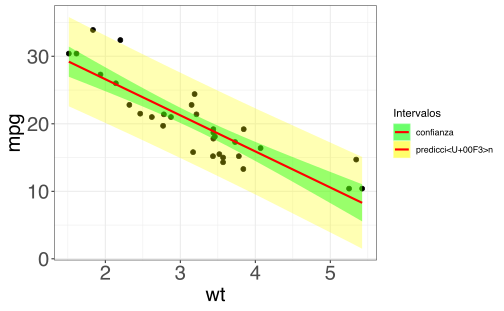
\includegraphics[width=0.7\linewidth]{Notas-Curso-Estadistica_files/figure-latex/unnamed-chunk-127-1} \end{center}

\begin{Shaded}
\begin{Highlighting}[]
\CommentTok{\# \# Guardar el gráfico en un archivo pdf}
\CommentTok{\# ggsave(filename = \textquotesingle{}linear\_reg\_con\_IC.pdf\textquotesingle{}) \# }
\end{Highlighting}
\end{Shaded}

\hypertarget{ajuste-de-la-regresiuxf3n-con-intervalos-de-confianza-y-predicciuxf3n}{%
\subsubsection{Ajuste de la regresión con intervalos de confianza y predicción}\label{ajuste-de-la-regresiuxf3n-con-intervalos-de-confianza-y-predicciuxf3n}}

\begin{Shaded}
\begin{Highlighting}[]
\CommentTok{\# Agregamos a mtcars el intervalo de predicción}
\CommentTok{\# para cada dato}
\NormalTok{mtcars.pred }\OtherTok{\textless{}{-}} \FunctionTok{data.frame}\NormalTok{(mtcars, }\FunctionTok{predict}\NormalTok{(lm.r, }\AttributeTok{interval =} \StringTok{"prediction"}\NormalTok{))}

\NormalTok{p }\OtherTok{\textless{}{-}} \FunctionTok{ggplot}\NormalTok{(mtcars.pred, }\FunctionTok{aes}\NormalTok{(}\AttributeTok{x =}\NormalTok{ wt, }\AttributeTok{y =}\NormalTok{ mpg))}
\CommentTok{\# Use circulos de tamaño 2}
\NormalTok{p }\OtherTok{\textless{}{-}}\NormalTok{ p }\SpecialCharTok{+} \FunctionTok{geom\_point}\NormalTok{(}\AttributeTok{size =} \DecValTok{2}\NormalTok{)}
\CommentTok{\# Agregue una banda de tamaño [lwr, upr] para}
\CommentTok{\# cada punto y llamela \textquotesingle{}predicción\textquotesingle{}}
\NormalTok{p }\OtherTok{\textless{}{-}}\NormalTok{ p }\SpecialCharTok{+} \FunctionTok{geom\_ribbon}\NormalTok{(}\FunctionTok{aes}\NormalTok{(}\AttributeTok{ymin =}\NormalTok{ lwr, }\AttributeTok{ymax =}\NormalTok{ upr, }\AttributeTok{fill =} \StringTok{"predicción"}\NormalTok{),}
    \AttributeTok{alpha =} \FloatTok{0.3}\NormalTok{)}
\CommentTok{\# Agregue el intervalo de confianza usual y llame}
\CommentTok{\# a ese intervalo \textquotesingle{}confianza\textquotesingle{}}
\NormalTok{p }\OtherTok{\textless{}{-}}\NormalTok{ p }\SpecialCharTok{+} \FunctionTok{geom\_smooth}\NormalTok{(}\AttributeTok{method =}\NormalTok{ lm, }\FunctionTok{aes}\NormalTok{(}\AttributeTok{fill =} \StringTok{"confianza"}\NormalTok{),}
    \AttributeTok{size =} \DecValTok{1}\NormalTok{, }\AttributeTok{col =} \StringTok{"red"}\NormalTok{)}
\CommentTok{\# Para agregar bien las leyendas}
\NormalTok{p }\OtherTok{\textless{}{-}}\NormalTok{ p }\SpecialCharTok{+} \FunctionTok{scale\_fill\_manual}\NormalTok{(}\StringTok{"Intervalos"}\NormalTok{, }\AttributeTok{values =} \FunctionTok{c}\NormalTok{(}\StringTok{"green"}\NormalTok{,}
    \StringTok{"yellow"}\NormalTok{))}
\NormalTok{p }\OtherTok{\textless{}{-}}\NormalTok{ p }\SpecialCharTok{+} \FunctionTok{theme\_bw}\NormalTok{()}
\NormalTok{p }\OtherTok{\textless{}{-}}\NormalTok{ p }\SpecialCharTok{+} \FunctionTok{theme}\NormalTok{(}\AttributeTok{axis.text =} \FunctionTok{element\_text}\NormalTok{(}\AttributeTok{size =} \DecValTok{20}\NormalTok{),}
    \AttributeTok{axis.title =} \FunctionTok{element\_text}\NormalTok{(}\AttributeTok{size =} \DecValTok{20}\NormalTok{))}

\CommentTok{\# Dibujar el gráfico}
\NormalTok{p}
\end{Highlighting}
\end{Shaded}

\begin{center}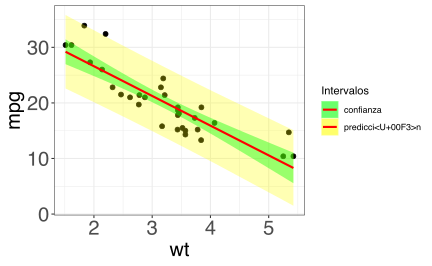
\includegraphics[width=0.7\linewidth]{Notas-Curso-Estadistica_files/figure-latex/unnamed-chunk-128-1} \end{center}

\begin{Shaded}
\begin{Highlighting}[]
\CommentTok{\# \# Guardar el gráfico en un archivo pdf}
\CommentTok{\# ggsave(filename = \textquotesingle{}linear\_reg\_con\_IC\_IP.pdf\textquotesingle{}) \#}
\end{Highlighting}
\end{Shaded}

Repitamos el mismo ejercicio anterior pero con un caso más sencillo.

\begin{Shaded}
\begin{Highlighting}[]
\NormalTok{n }\OtherTok{\textless{}{-}} \DecValTok{1000}

\NormalTok{X }\OtherTok{\textless{}{-}} \FunctionTok{runif}\NormalTok{(n, }\DecValTok{0}\NormalTok{, }\DecValTok{10}\NormalTok{)}
\NormalTok{Y }\OtherTok{\textless{}{-}} \DecValTok{10} \SpecialCharTok{+} \FunctionTok{sin}\NormalTok{(}\DecValTok{5} \SpecialCharTok{*}\NormalTok{ X) }\SpecialCharTok{+}\NormalTok{ X }\SpecialCharTok{+} \FunctionTok{rnorm}\NormalTok{(}\DecValTok{1000}\NormalTok{, }\DecValTok{0}\NormalTok{, }\DecValTok{1}\NormalTok{)}
\NormalTok{toyex.initial }\OtherTok{\textless{}{-}} \FunctionTok{data.frame}\NormalTok{(X, Y) }\SpecialCharTok{\%\textgreater{}\%}
    \FunctionTok{arrange}\NormalTok{(X)}

\FunctionTok{plot}\NormalTok{(toyex.initial)}
\end{Highlighting}
\end{Shaded}

\begin{center}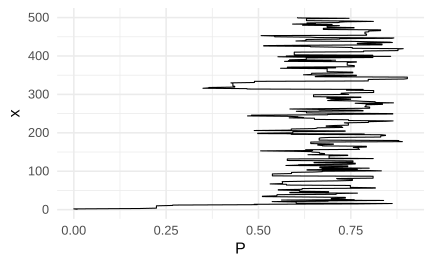
\includegraphics[width=0.7\linewidth]{Notas-Curso-Estadistica_files/figure-latex/unnamed-chunk-129-1} \end{center}

\begin{Shaded}
\begin{Highlighting}[]
\NormalTok{lm.toyex.initial }\OtherTok{\textless{}{-}} \FunctionTok{lm}\NormalTok{(Y }\SpecialCharTok{\textasciitilde{}}\NormalTok{ X, }\AttributeTok{data =}\NormalTok{ toyex.initial)}

\FunctionTok{summary}\NormalTok{(lm.toyex.initial)}
\end{Highlighting}
\end{Shaded}

\begin{verbatim}
## 
## Call:
## lm(formula = Y ~ X, data = toyex.initial)
## 
## Residuals:
##     Min      1Q  Median      3Q     Max 
## -3.4587 -0.8232  0.0468  0.8709  3.4115 
## 
## Coefficients:
##             Estimate Std. Error t value Pr(>|t|)    
## (Intercept) 10.01402    0.07847  127.61   <2e-16 ***
## X            0.98895    0.01340   73.81   <2e-16 ***
## ---
## Signif. codes:  0 '***' 0.001 '**' 0.01 '*' 0.05 '.' 0.1 ' ' 1
## 
## Residual standard error: 1.208 on 998 degrees of freedom
## Multiple R-squared:  0.8452, Adjusted R-squared:  0.845 
## F-statistic:  5448 on 1 and 998 DF,  p-value: < 2.2e-16
\end{verbatim}

\begin{Shaded}
\begin{Highlighting}[]
\NormalTok{toyex.pred.initial }\OtherTok{\textless{}{-}} \FunctionTok{data.frame}\NormalTok{(toyex.initial, }\FunctionTok{predict}\NormalTok{(lm.toyex.initial,}
    \AttributeTok{interval =} \StringTok{"prediction"}\NormalTok{))}
\end{Highlighting}
\end{Shaded}

Ahora, quisiera generar muchas muestras del mismo experimento

\begin{Shaded}
\begin{Highlighting}[]
\NormalTok{toyex.pred }\OtherTok{\textless{}{-}} \ConstantTok{NULL}

\ControlFlowTok{for}\NormalTok{ (i }\ControlFlowTok{in} \DecValTok{1}\SpecialCharTok{:}\DecValTok{10}\NormalTok{) \{}
\NormalTok{    X }\OtherTok{\textless{}{-}} \FunctionTok{runif}\NormalTok{(n, }\DecValTok{0}\NormalTok{, }\DecValTok{10}\NormalTok{)}
\NormalTok{    Y }\OtherTok{\textless{}{-}} \DecValTok{10} \SpecialCharTok{+} \FunctionTok{sin}\NormalTok{(}\DecValTok{5} \SpecialCharTok{*}\NormalTok{ X) }\SpecialCharTok{+}\NormalTok{ X }\SpecialCharTok{+} \FunctionTok{rnorm}\NormalTok{(}\DecValTok{1000}\NormalTok{, }\DecValTok{0}\NormalTok{, }\DecValTok{1}\NormalTok{)}
\NormalTok{    toyexi }\OtherTok{\textless{}{-}} \FunctionTok{data.frame}\NormalTok{(}\AttributeTok{im =}\NormalTok{ i, X, Y)}
\NormalTok{    toyexi }\OtherTok{\textless{}{-}}\NormalTok{ toyexi }\SpecialCharTok{\%\textgreater{}\%}
        \FunctionTok{arrange}\NormalTok{(X)}
\NormalTok{    toyex.pred }\OtherTok{\textless{}{-}} \FunctionTok{bind\_rows}\NormalTok{(toyex.pred, }\FunctionTok{data.frame}\NormalTok{(toyexi,}
        \FunctionTok{predict}\NormalTok{(lm.toyex.initial, }\AttributeTok{interval =} \StringTok{"prediction"}\NormalTok{)))}
\NormalTok{\}}


\ControlFlowTok{for}\NormalTok{ (i }\ControlFlowTok{in} \DecValTok{1}\SpecialCharTok{:}\DecValTok{10}\NormalTok{) \{}
\NormalTok{    toyex.pred}\SpecialCharTok{$}\NormalTok{fit }\OtherTok{\textless{}{-}} \FunctionTok{fitted}\NormalTok{(}\FunctionTok{lm}\NormalTok{(}\AttributeTok{formula =}\NormalTok{ Y }\SpecialCharTok{\textasciitilde{}}\NormalTok{ X, }\AttributeTok{data =}\NormalTok{ toyex.pred[toyex.pred}\SpecialCharTok{$}\NormalTok{im }\SpecialCharTok{==}
\NormalTok{        i, ]))}
\NormalTok{\}}

\NormalTok{toyex.pred}\SpecialCharTok{$}\NormalTok{im }\OtherTok{\textless{}{-}} \FunctionTok{as.factor}\NormalTok{(toyex.pred}\SpecialCharTok{$}\NormalTok{im)}
\end{Highlighting}
\end{Shaded}

\begin{Shaded}
\begin{Highlighting}[]
\FunctionTok{library}\NormalTok{(gganimate)}

\FunctionTok{ggplot}\NormalTok{(}\AttributeTok{data =}\NormalTok{ toyex.pred, }\FunctionTok{aes}\NormalTok{(}\AttributeTok{x =}\NormalTok{ X, }\AttributeTok{y =}\NormalTok{ Y)) }\SpecialCharTok{+} \FunctionTok{geom\_point}\NormalTok{(}\AttributeTok{size =} \DecValTok{1}\NormalTok{) }\SpecialCharTok{+}
    \FunctionTok{geom\_smooth}\NormalTok{(}\AttributeTok{data =}\NormalTok{ toyex.initial, }\AttributeTok{method =}\NormalTok{ lm,}
        \AttributeTok{mapping =} \FunctionTok{aes}\NormalTok{(}\AttributeTok{fill =} \StringTok{"confianza"}\NormalTok{), }\AttributeTok{size =} \DecValTok{1}\NormalTok{,}
        \AttributeTok{col =} \StringTok{"red"}\NormalTok{) }\SpecialCharTok{+} \FunctionTok{geom\_ribbon}\NormalTok{(}\AttributeTok{data =}\NormalTok{ toyex.pred.initial,}
    \AttributeTok{mapping =} \FunctionTok{aes}\NormalTok{(}\AttributeTok{x =}\NormalTok{ X, }\AttributeTok{ymin =}\NormalTok{ lwr, }\AttributeTok{ymax =}\NormalTok{ upr, }\AttributeTok{fill =} \StringTok{"predicción"}\NormalTok{,}
\NormalTok{        ), }\AttributeTok{alpha =} \FloatTok{0.3}\NormalTok{) }\SpecialCharTok{+} \FunctionTok{labs}\NormalTok{(}\AttributeTok{title =} \FunctionTok{paste0}\NormalTok{(}\StringTok{"Muestra \#: \{closest\_state\}"}\NormalTok{)) }\SpecialCharTok{+}
    \FunctionTok{scale\_fill\_manual}\NormalTok{(}\StringTok{"Intervalos"}\NormalTok{, }\AttributeTok{values =} \FunctionTok{c}\NormalTok{(}\StringTok{"green"}\NormalTok{,}
        \StringTok{"yellow"}\NormalTok{)) }\SpecialCharTok{+} \FunctionTok{theme\_bw}\NormalTok{() }\SpecialCharTok{+} \FunctionTok{theme}\NormalTok{(}\AttributeTok{axis.text =} \FunctionTok{element\_text}\NormalTok{(}\AttributeTok{size =} \DecValTok{20}\NormalTok{),}
    \AttributeTok{axis.title =} \FunctionTok{element\_text}\NormalTok{(}\AttributeTok{size =} \DecValTok{20}\NormalTok{)) }\SpecialCharTok{+} \FunctionTok{transition\_states}\NormalTok{(im)}
\end{Highlighting}
\end{Shaded}

\hypertarget{interacciones}{%
\section{Interacciones}\label{interacciones}}

Suponga un modelo lineal con dos covariables:

\begin{equation*}
Y = \beta_{0} + \beta_{1} X_{1} + \beta_{2} X_{2} + \varepsilon
\end{equation*}

Aumentemos en 1 unidad \(X_{1}\) y rescribamos el modelo original

\begin{align*}
Y &=  \beta_{0} + \beta_{1} (X_{1}+1) + \beta_{2} X_{2} + \varepsilon \\
Y &=  (\beta_{0} + \beta_{1}) + \beta_{1} X_{1} + \beta_{2} X_{2} + \varepsilon \\
Y &=  \tilde{\beta_{0}} + \beta_{1} X_{1} + \beta_{2} X_{2} + \varepsilon \\
\end{align*}

Es decir, el modelo original sigue siendo teniendo la misma estructura aunque hayamos cambiado el \(X_1\). Este fenómeno ocurre siempre bajo transformaciones lineales de las variables.

Ahora suponga que tenemos el siguiente modelo:
\begin{align*}
Y =  \beta_{0} + \beta_{1} X_{1} X_{2} +\varepsilon \\
\end{align*}

y aumentamos en 1 el \(X_1\):

\begin{align*}
Y &=  \beta_{0} + \beta_{1} (X_{1}+1) X_{2} +\varepsilon \\
Y &=  \beta_{0} + \beta_{1}X_{2} +  \beta_{1} X_{1} X_{2} +\varepsilon \\
\end{align*}

Note que en este caso no se logra mantener el mismo tipo de estructura. Una forma de arreglar el problema es incluir las \emph{interacciones} junto con todos sus \emph{efectos principales}.

\begin{equation*}
Y =  \beta_{0} + \beta_{1}X_{1} + \beta_{2} X_{2} +  \beta_{3} X_{1} X_{2} +\varepsilon \\
\end{equation*}

Este modelo se le conoce como modelo lineal con interacciones (caso de 2 covariables). Este modelo considera la posible interacción entre las covariables \(X_1\) y \(X_2\) que permiten cambiar tanto el intercepto como las pendientes de los efectos principales.

\textbf{Principio de jerarquía}. Con el fin de mantener la estructura del modelo lineal, siempre es necesario incluir los efectos principales cuando se determina que una interacción entre ellos es significativa.

\begin{exercise}
\protect\hypertarget{exr:unnamed-chunk-133}{}\label{exr:unnamed-chunk-133}Compruebe que para el caso anterior, si aumenta en una unidad \(X_{1}\), el modelo preserva su estructura.
\end{exercise}

\hypertarget{laboratorio-5}{%
\subsection{Laboratorio}\label{laboratorio-5}}

Generamos una base de datos nueva con solamente \texttt{wt} centrado

\begin{Shaded}
\begin{Highlighting}[]
\CommentTok{\# La función across y where solo funciona solo}
\CommentTok{\# para dplyr 1.0 Si tienen otra versión, pueden}
\CommentTok{\# usar mutate\_if}

\NormalTok{mtcars\_centered }\OtherTok{\textless{}{-}}\NormalTok{ mtcars }\SpecialCharTok{\%\textgreater{}\%}
    \FunctionTok{mutate}\NormalTok{(}\FunctionTok{across}\NormalTok{(}\StringTok{"wt"}\NormalTok{, scale, }\AttributeTok{scale =} \ConstantTok{FALSE}\NormalTok{, }\AttributeTok{center =} \ConstantTok{TRUE}\NormalTok{))}

\CommentTok{\# Si no se tiene dplyr 1.0}

\NormalTok{mtcars\_centered }\OtherTok{\textless{}{-}}\NormalTok{ mtcars }\SpecialCharTok{\%\textgreater{}\%}
    \FunctionTok{mutate\_at}\NormalTok{(}\StringTok{"wt"}\NormalTok{, scale, }\AttributeTok{scale =} \ConstantTok{FALSE}\NormalTok{, }\AttributeTok{center =} \ConstantTok{TRUE}\NormalTok{)}
\end{Highlighting}
\end{Shaded}

Compare lo que ocurre con los coeficientes de la base original y la nueva base.

\begin{Shaded}
\begin{Highlighting}[]
\FunctionTok{summary}\NormalTok{(}\FunctionTok{lm}\NormalTok{(mpg }\SpecialCharTok{\textasciitilde{}}\NormalTok{ wt }\SpecialCharTok{+}\NormalTok{ disp, }\AttributeTok{data =}\NormalTok{ mtcars))}
\end{Highlighting}
\end{Shaded}

\begin{verbatim}
## 
## Call:
## lm(formula = mpg ~ wt + disp, data = mtcars)
## 
## Residuals:
##     Min      1Q  Median      3Q     Max 
## -3.4087 -2.3243 -0.7683  1.7721  6.3484 
## 
## Coefficients:
##             Estimate Std. Error t value Pr(>|t|)    
## (Intercept) 34.96055    2.16454  16.151 4.91e-16 ***
## wt          -3.35082    1.16413  -2.878  0.00743 ** 
## disp        -0.01773    0.00919  -1.929  0.06362 .  
## ---
## Signif. codes:  0 '***' 0.001 '**' 0.01 '*' 0.05 '.' 0.1 ' ' 1
## 
## Residual standard error: 2.917 on 29 degrees of freedom
## Multiple R-squared:  0.7809, Adjusted R-squared:  0.7658 
## F-statistic: 51.69 on 2 and 29 DF,  p-value: 2.744e-10
\end{verbatim}

\begin{Shaded}
\begin{Highlighting}[]
\FunctionTok{summary}\NormalTok{(}\FunctionTok{lm}\NormalTok{(mpg }\SpecialCharTok{\textasciitilde{}}\NormalTok{ wt }\SpecialCharTok{+}\NormalTok{ disp, }\AttributeTok{data =}\NormalTok{ mtcars\_centered))}
\end{Highlighting}
\end{Shaded}

\begin{verbatim}
## 
## Call:
## lm(formula = mpg ~ wt + disp, data = mtcars_centered)
## 
## Residuals:
##     Min      1Q  Median      3Q     Max 
## -3.4087 -2.3243 -0.7683  1.7721  6.3484 
## 
## Coefficients:
##             Estimate Std. Error t value Pr(>|t|)    
## (Intercept) 24.18011    2.18221  11.081 6.12e-12 ***
## wt          -3.35082    1.16413  -2.878  0.00743 ** 
## disp        -0.01773    0.00919  -1.929  0.06362 .  
## ---
## Signif. codes:  0 '***' 0.001 '**' 0.01 '*' 0.05 '.' 0.1 ' ' 1
## 
## Residual standard error: 2.917 on 29 degrees of freedom
## Multiple R-squared:  0.7809, Adjusted R-squared:  0.7658 
## F-statistic: 51.69 on 2 and 29 DF,  p-value: 2.744e-10
\end{verbatim}

Supongamos que formamos un modelo con solo la interacción y no incluimos los efectos directos.

\begin{Shaded}
\begin{Highlighting}[]
\FunctionTok{summary}\NormalTok{(}\FunctionTok{lm}\NormalTok{(mpg }\SpecialCharTok{\textasciitilde{}}\NormalTok{ wt }\SpecialCharTok{*}\NormalTok{ disp }\SpecialCharTok{{-}}\NormalTok{ wt }\SpecialCharTok{{-}}\NormalTok{ disp, }\AttributeTok{data =}\NormalTok{ mtcars))}
\end{Highlighting}
\end{Shaded}

\begin{verbatim}
## 
## Call:
## lm(formula = mpg ~ wt * disp - wt - disp, data = mtcars)
## 
## Residuals:
##    Min     1Q Median     3Q    Max 
## -4.259 -2.603 -1.657  2.165  8.589 
## 
## Coefficients:
##               Estimate Std. Error t value Pr(>|t|)    
## (Intercept) 26.2621926  1.0418029  25.208  < 2e-16 ***
## wt:disp     -0.0072897  0.0009721  -7.499 2.33e-08 ***
## ---
## Signif. codes:  0 '***' 0.001 '**' 0.01 '*' 0.05 '.' 0.1 ' ' 1
## 
## Residual standard error: 3.614 on 30 degrees of freedom
## Multiple R-squared:  0.6521, Adjusted R-squared:  0.6405 
## F-statistic: 56.24 on 1 and 30 DF,  p-value: 2.329e-08
\end{verbatim}

\begin{Shaded}
\begin{Highlighting}[]
\FunctionTok{summary}\NormalTok{(}\FunctionTok{lm}\NormalTok{(mpg }\SpecialCharTok{\textasciitilde{}}\NormalTok{ wt }\SpecialCharTok{*}\NormalTok{ disp }\SpecialCharTok{{-}}\NormalTok{ wt }\SpecialCharTok{{-}}\NormalTok{ disp, }\AttributeTok{data =}\NormalTok{ mtcars\_centered))}
\end{Highlighting}
\end{Shaded}

\begin{verbatim}
## 
## Call:
## lm(formula = mpg ~ wt * disp - wt - disp, data = mtcars_centered)
## 
## Residuals:
##    Min     1Q Median     3Q    Max 
## -5.878 -2.775 -1.162  2.409 11.150 
## 
## Coefficients:
##              Estimate Std. Error t value Pr(>|t|)    
## (Intercept) 21.460008   0.859706  24.962  < 2e-16 ***
## wt:disp     -0.013127   0.002714  -4.837 3.69e-05 ***
## ---
## Signif. codes:  0 '***' 0.001 '**' 0.01 '*' 0.05 '.' 0.1 ' ' 1
## 
## Residual standard error: 4.592 on 30 degrees of freedom
## Multiple R-squared:  0.4382, Adjusted R-squared:  0.4195 
## F-statistic:  23.4 on 1 and 30 DF,  p-value: 3.686e-05
\end{verbatim}

El modelo correcto sería el siguiente:

\begin{Shaded}
\begin{Highlighting}[]
\FunctionTok{summary}\NormalTok{(}\FunctionTok{lm}\NormalTok{(mpg }\SpecialCharTok{\textasciitilde{}}\NormalTok{ wt }\SpecialCharTok{+}\NormalTok{ disp }\SpecialCharTok{+}\NormalTok{ wt }\SpecialCharTok{*}\NormalTok{ disp, }\AttributeTok{data =}\NormalTok{ mtcars))}
\end{Highlighting}
\end{Shaded}

\begin{verbatim}
## 
## Call:
## lm(formula = mpg ~ wt + disp + wt * disp, data = mtcars)
## 
## Residuals:
##    Min     1Q Median     3Q    Max 
## -3.267 -1.677 -0.836  1.351  5.017 
## 
## Coefficients:
##              Estimate Std. Error t value Pr(>|t|)    
## (Intercept) 44.081998   3.123063  14.115 2.96e-14 ***
## wt          -6.495680   1.313383  -4.946 3.22e-05 ***
## disp        -0.056358   0.013239  -4.257  0.00021 ***
## wt:disp      0.011705   0.003255   3.596  0.00123 ** 
## ---
## Signif. codes:  0 '***' 0.001 '**' 0.01 '*' 0.05 '.' 0.1 ' ' 1
## 
## Residual standard error: 2.455 on 28 degrees of freedom
## Multiple R-squared:  0.8501, Adjusted R-squared:  0.8341 
## F-statistic: 52.95 on 3 and 28 DF,  p-value: 1.158e-11
\end{verbatim}

\begin{Shaded}
\begin{Highlighting}[]
\FunctionTok{summary}\NormalTok{(}\FunctionTok{lm}\NormalTok{(mpg }\SpecialCharTok{\textasciitilde{}}\NormalTok{ wt }\SpecialCharTok{+}\NormalTok{ disp }\SpecialCharTok{+}\NormalTok{ wt }\SpecialCharTok{*}\NormalTok{ disp, }\AttributeTok{data =}\NormalTok{ mtcars\_centered))}
\end{Highlighting}
\end{Shaded}

\begin{verbatim}
## 
## Call:
## lm(formula = mpg ~ wt + disp + wt * disp, data = mtcars_centered)
## 
## Residuals:
##    Min     1Q Median     3Q    Max 
## -3.267 -1.677 -0.836  1.351  5.017 
## 
## Coefficients:
##              Estimate Std. Error t value Pr(>|t|)    
## (Intercept) 23.183772   1.857605  12.480 5.87e-13 ***
## wt          -6.495680   1.313383  -4.946 3.22e-05 ***
## disp        -0.018699   0.007741  -2.416  0.02248 *  
## wt:disp      0.011705   0.003255   3.596  0.00123 ** 
## ---
## Signif. codes:  0 '***' 0.001 '**' 0.01 '*' 0.05 '.' 0.1 ' ' 1
## 
## Residual standard error: 2.455 on 28 degrees of freedom
## Multiple R-squared:  0.8501, Adjusted R-squared:  0.8341 
## F-statistic: 52.95 on 3 and 28 DF,  p-value: 1.158e-11
\end{verbatim}

\begin{exercise}

Repita los comandos anteriores con la siguiente base de datos y explique los resultados.

\begin{Shaded}
\begin{Highlighting}[]
\NormalTok{mtcars\_scaled }\OtherTok{\textless{}{-}}\NormalTok{ mtcars }\SpecialCharTok{\%\textgreater{}\%}
    \FunctionTok{mutate}\NormalTok{(}\FunctionTok{across}\NormalTok{(}\FunctionTok{c}\NormalTok{(}\StringTok{"wt"}\NormalTok{, }\StringTok{"disp"}\NormalTok{), scale, }\AttributeTok{scale =} \ConstantTok{TRUE}\NormalTok{,}
        \AttributeTok{center =} \ConstantTok{TRUE}\NormalTok{))}
\end{Highlighting}
\end{Shaded}

\end{exercise}

\hypertarget{supuestos}{%
\section{Supuestos}\label{supuestos}}

El modelo lineal tiene los siguientes supuestos:

\begin{description}
\tightlist
\item[Linealidad]
En la forma lineal de la relación variable dependiente-covariables.
\item[Errores centrados]
\(\mathbb{E}(\varepsilon_i) = 0\).
\item[Homocedasticidad]
\(\text{Var}(\varepsilon_t) = \mathbb{E}(\varepsilon_t - \mathbb{E} \varepsilon_t)^2 = \mathbb{E} \varepsilon_t^2 = \sigma^2\) para todo \(t\). Es decir, la varianza del modelo (\textbf{error irreducible}) no depende de las variables independientes u otro factor.
\item[Normalidad de los residuos]
\(\varepsilon \sim N(0, \sigma^2 )\).
\item[Independencia de los errores]
\(\text{Cov}(\varepsilon_t,\varepsilon_s ) = \mathbb{E} (\varepsilon_t - \mathbb{E} \varepsilon_t) (\varepsilon_s - \mathbb{E} \varepsilon_s) = \mathbb{E} \varepsilon_t \varepsilon_s = 0\) para todo \(t,s\) con \(t\neq s\): si para una observación dada existe un error, este no debe depender del error de otra observación.
\end{description}

Si este supuesto no se cumple puede provocar que los errores estándar en intervalos de confianza y predicción sean subestimados. Es decir que un intervalo del 95\% tendrá un margen de error menor y se rechazaría más fácilmente la hipotesis nula de las pruebas \(t\) y \(F\).

\begin{description}
\tightlist
\item[Multicolinealidad]
Se asume que la matriz \(X^TX\) es invertible, es decir \(X\) es una matriz de rango completo. Para esto cada una las covariables no debe ser linealmente dependientes, es decir \(X^TX\) de debe acercarse a ser a una matriz singular con determinante cercano a 0. Es decir que cada variable explica aproximadamente ``un aspecto o característica'' del modelo. Sin embargo puede pasar que varias variables expliquen la misma característica y el modelo se vuelve \textbf{inestable} por decidir entre las dos variables. Por ejemplo: la temperatura en grados centigrados y farenheit.
\end{description}

Esto generaría que \(\mathrm{Var}\left(\beta\right)\) sea alto ya que
\begin{equation*}
\text{Var}(\beta) =  \sigma^2(X^{\top}X)^{-1}
\end{equation*}

\begin{description}
\tightlist
\item[Más observaciones que predictores]
En caso contrario existen formas alternativas de definir el problema de regresión. (Volveremos a esto cuando veamos selección de modelos)
\end{description}

\hypertarget{chequeos-buxe1sicos-de-las-hipuxf3tesis-de-regresiuxf3n-lineal}{%
\subsection{Chequeos básicos de las hipótesis de regresión lineal}\label{chequeos-buxe1sicos-de-las-hipuxf3tesis-de-regresiuxf3n-lineal}}

\hypertarget{linealidad-errores-con-esperanza-nula-homocedasticidad}{%
\subsubsection{Linealidad, Errores con esperanza nula, Homocedasticidad}\label{linealidad-errores-con-esperanza-nula-homocedasticidad}}

Estos supuestos se puede constantar a partir de un gráfico de residuos ya que en el caso ideal \(e_{i} = \hat{Y}_{i}- Y_{i} \perp \hat{Y}_{i}\). Entonces si este gráfico presenta patrones, quiere indicar que la regresión, no es lineal, que los errores no tienen esperanza nula y que la varianza no es constante.

Se pueden aplicar transformaciones para resolver estos problemas. Normalmente se usan transformaciones como raiz cuadrada o logaritmos.

\begin{example}

\textbf{Caso ideal}

\begin{Shaded}
\begin{Highlighting}[]
\NormalTok{x }\OtherTok{\textless{}{-}} \FunctionTok{rnorm}\NormalTok{(}\DecValTok{1000}\NormalTok{)}
\NormalTok{y }\OtherTok{\textless{}{-}}\NormalTok{ x }\SpecialCharTok{+} \FunctionTok{rnorm}\NormalTok{(}\DecValTok{1000}\NormalTok{, }\AttributeTok{sd =} \FloatTok{0.5}\NormalTok{)}

\NormalTok{fit }\OtherTok{\textless{}{-}} \FunctionTok{lm}\NormalTok{(y }\SpecialCharTok{\textasciitilde{}}\NormalTok{ x)}
\FunctionTok{plot}\NormalTok{(x, y)}
\FunctionTok{abline}\NormalTok{(}\AttributeTok{a =} \FunctionTok{coef}\NormalTok{(fit)[}\DecValTok{1}\NormalTok{], }\AttributeTok{b =} \FunctionTok{coef}\NormalTok{(fit)[}\DecValTok{2}\NormalTok{], }\AttributeTok{col =} \StringTok{"red"}\NormalTok{)}
\end{Highlighting}
\end{Shaded}

\begin{center}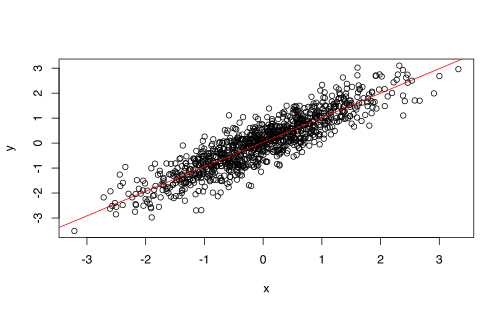
\includegraphics[width=0.7\linewidth]{Notas-Curso-Estadistica_files/figure-latex/unnamed-chunk-139-1} \end{center}

\begin{Shaded}
\begin{Highlighting}[]
\FunctionTok{plot}\NormalTok{(}\FunctionTok{fitted}\NormalTok{(fit), }\FunctionTok{residuals}\NormalTok{(fit))}
\FunctionTok{abline}\NormalTok{(}\AttributeTok{h =} \DecValTok{0}\NormalTok{, }\AttributeTok{col =} \StringTok{"red"}\NormalTok{)}
\end{Highlighting}
\end{Shaded}

\begin{figure}

{\centering 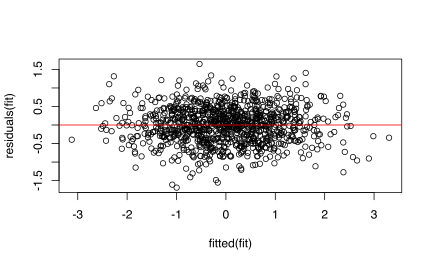
\includegraphics[width=0.7\linewidth]{Notas-Curso-Estadistica_files/figure-latex/grafico-residuos-lineal-1} 

}

\caption{Gráfico de residuos caso lineal}\label{fig:grafico-residuos-lineal}
\end{figure}

\textbf{Caso no-lineal}

\begin{Shaded}
\begin{Highlighting}[]
\NormalTok{x }\OtherTok{\textless{}{-}} \FunctionTok{exp}\NormalTok{(}\FunctionTok{rnorm}\NormalTok{(}\DecValTok{1000}\NormalTok{))}
\NormalTok{y }\OtherTok{\textless{}{-}} \FunctionTok{log}\NormalTok{(x) }\SpecialCharTok{+} \FunctionTok{rnorm}\NormalTok{(}\DecValTok{1000}\NormalTok{, }\AttributeTok{sd =} \FloatTok{0.5}\NormalTok{)}

\NormalTok{fit }\OtherTok{\textless{}{-}} \FunctionTok{lm}\NormalTok{(y }\SpecialCharTok{\textasciitilde{}}\NormalTok{ x)}
\FunctionTok{plot}\NormalTok{(x, y)}
\FunctionTok{abline}\NormalTok{(}\AttributeTok{a =} \FunctionTok{coef}\NormalTok{(fit)[}\DecValTok{1}\NormalTok{], }\AttributeTok{b =} \FunctionTok{coef}\NormalTok{(fit)[}\DecValTok{2}\NormalTok{], }\AttributeTok{col =} \StringTok{"red"}\NormalTok{)}
\end{Highlighting}
\end{Shaded}

\begin{center}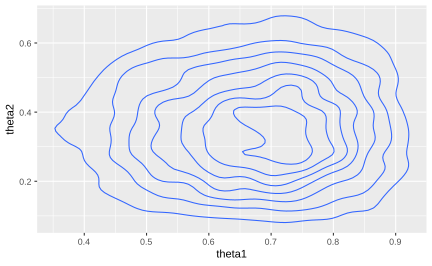
\includegraphics[width=0.7\linewidth]{Notas-Curso-Estadistica_files/figure-latex/unnamed-chunk-140-1} \end{center}

\begin{Shaded}
\begin{Highlighting}[]
\FunctionTok{plot}\NormalTok{(}\FunctionTok{fitted}\NormalTok{(fit), }\FunctionTok{residuals}\NormalTok{(fit))}
\FunctionTok{abline}\NormalTok{(}\AttributeTok{h =} \DecValTok{0}\NormalTok{, }\AttributeTok{col =} \StringTok{"red"}\NormalTok{)}
\end{Highlighting}
\end{Shaded}

\begin{figure}

{\centering \includegraphics[width=0.7\linewidth]{Notas-Curso-Estadistica_files/figure-latex/grafico-residuos-no-lineal-1} 

}

\caption{Gráfico de residuos caso no-lineal}\label{fig:grafico-residuos-no-lineal}
\end{figure}

\textbf{Caso no-lineal transformado}

\begin{Shaded}
\begin{Highlighting}[]
\NormalTok{xt }\OtherTok{\textless{}{-}} \FunctionTok{log}\NormalTok{(x)}


\NormalTok{fit }\OtherTok{\textless{}{-}} \FunctionTok{lm}\NormalTok{(y }\SpecialCharTok{\textasciitilde{}}\NormalTok{ xt)}
\FunctionTok{plot}\NormalTok{(xt, y)}
\FunctionTok{abline}\NormalTok{(}\AttributeTok{a =} \FunctionTok{coef}\NormalTok{(fit)[}\DecValTok{1}\NormalTok{], }\AttributeTok{b =} \FunctionTok{coef}\NormalTok{(fit)[}\DecValTok{2}\NormalTok{], }\AttributeTok{col =} \StringTok{"red"}\NormalTok{)}
\end{Highlighting}
\end{Shaded}

\begin{center}\includegraphics[width=0.7\linewidth]{Notas-Curso-Estadistica_files/figure-latex/unnamed-chunk-141-1} \end{center}

\begin{Shaded}
\begin{Highlighting}[]
\FunctionTok{plot}\NormalTok{(}\FunctionTok{fitted}\NormalTok{(fit), }\FunctionTok{residuals}\NormalTok{(fit))}
\FunctionTok{abline}\NormalTok{(}\AttributeTok{h =} \DecValTok{0}\NormalTok{, }\AttributeTok{col =} \StringTok{"red"}\NormalTok{)}
\end{Highlighting}
\end{Shaded}

\begin{center}\includegraphics[width=0.7\linewidth]{Notas-Curso-Estadistica_files/figure-latex/unnamed-chunk-141-2} \end{center}

\end{example}

\hypertarget{independencia-de-los-errores}{%
\subsubsection{Independencia de los errores}\label{independencia-de-los-errores}}

En este caso defina \(\rho(k) = \text{Cov}(\varepsilon_i,\varepsilon_{i+k} )\). Si los residuos son independientes, entonces debe ocurrir que

\begin{equation*}
\rho(k) = \begin{cases}
1 & k=0\\
0 & k\neq 0.
\end{cases}  
\end{equation*}

Se calcula la función de autocorrelación empírica y se grafica para analizar su comportamiento

\textbf{Caso ideal}

\begin{Shaded}
\begin{Highlighting}[]
\NormalTok{x }\OtherTok{\textless{}{-}} \FunctionTok{rnorm}\NormalTok{(}\DecValTok{1000}\NormalTok{)}
\NormalTok{y }\OtherTok{\textless{}{-}} \DecValTok{1} \SpecialCharTok{+}\NormalTok{ x }\SpecialCharTok{+} \FunctionTok{rnorm}\NormalTok{(}\DecValTok{1000}\NormalTok{, }\AttributeTok{sd =} \DecValTok{1}\NormalTok{)}
\end{Highlighting}
\end{Shaded}

\begin{Shaded}
\begin{Highlighting}[]
\NormalTok{fit }\OtherTok{\textless{}{-}} \FunctionTok{lm}\NormalTok{(y }\SpecialCharTok{\textasciitilde{}}\NormalTok{ x)}
\FunctionTok{plot}\NormalTok{(x, y)}
\FunctionTok{abline}\NormalTok{(}\AttributeTok{a =} \FunctionTok{coef}\NormalTok{(fit)[}\DecValTok{1}\NormalTok{], }\AttributeTok{b =} \FunctionTok{coef}\NormalTok{(fit)[}\DecValTok{2}\NormalTok{], }\AttributeTok{col =} \StringTok{"red"}\NormalTok{)}
\end{Highlighting}
\end{Shaded}

\begin{center}\includegraphics[width=0.7\linewidth]{Notas-Curso-Estadistica_files/figure-latex/unnamed-chunk-143-1} \end{center}

\begin{Shaded}
\begin{Highlighting}[]
\FunctionTok{summary}\NormalTok{(fit)}
\end{Highlighting}
\end{Shaded}

\begin{verbatim}
## 
## Call:
## lm(formula = y ~ x)
## 
## Residuals:
##     Min      1Q  Median      3Q     Max 
## -3.2665 -0.6871  0.0002  0.6670  2.9410 
## 
## Coefficients:
##             Estimate Std. Error t value Pr(>|t|)    
## (Intercept)  1.04643    0.03183   32.87   <2e-16 ***
## x            0.95650    0.03287   29.10   <2e-16 ***
## ---
## Signif. codes:  0 '***' 0.001 '**' 0.01 '*' 0.05 '.' 0.1 ' ' 1
## 
## Residual standard error: 1.007 on 998 degrees of freedom
## Multiple R-squared:  0.4589, Adjusted R-squared:  0.4584 
## F-statistic: 846.6 on 1 and 998 DF,  p-value: < 2.2e-16
\end{verbatim}

\begin{Shaded}
\begin{Highlighting}[]
\FunctionTok{acf}\NormalTok{(}\FunctionTok{residuals}\NormalTok{(fit))}
\end{Highlighting}
\end{Shaded}

\begin{center}\includegraphics[width=0.7\linewidth]{Notas-Curso-Estadistica_files/figure-latex/unnamed-chunk-144-1} \end{center}

\textbf{Caso errores auto-correlacionados}

\begin{Shaded}
\begin{Highlighting}[]
\NormalTok{x }\OtherTok{\textless{}{-}} \FunctionTok{rnorm}\NormalTok{(}\DecValTok{1000}\NormalTok{)}
\NormalTok{y }\OtherTok{\textless{}{-}} \DecValTok{1} \SpecialCharTok{+}\NormalTok{ x }\SpecialCharTok{+} \FunctionTok{diffinv}\NormalTok{(}\FunctionTok{rnorm}\NormalTok{(}\DecValTok{999}\NormalTok{, }\AttributeTok{sd =} \DecValTok{1}\NormalTok{), }\AttributeTok{lag =} \DecValTok{1}\NormalTok{)}
\end{Highlighting}
\end{Shaded}

\begin{Shaded}
\begin{Highlighting}[]
\NormalTok{fit }\OtherTok{\textless{}{-}} \FunctionTok{lm}\NormalTok{(y }\SpecialCharTok{\textasciitilde{}}\NormalTok{ x)}
\FunctionTok{plot}\NormalTok{(x, y)}
\FunctionTok{abline}\NormalTok{(}\AttributeTok{a =} \FunctionTok{coef}\NormalTok{(fit)[}\DecValTok{1}\NormalTok{], }\AttributeTok{b =} \FunctionTok{coef}\NormalTok{(fit)[}\DecValTok{2}\NormalTok{], }\AttributeTok{col =} \StringTok{"red"}\NormalTok{)}
\end{Highlighting}
\end{Shaded}

\begin{center}\includegraphics[width=0.7\linewidth]{Notas-Curso-Estadistica_files/figure-latex/unnamed-chunk-146-1} \end{center}

\begin{Shaded}
\begin{Highlighting}[]
\FunctionTok{summary}\NormalTok{(fit)}
\end{Highlighting}
\end{Shaded}

\begin{verbatim}
## 
## Call:
## lm(formula = y ~ x)
## 
## Residuals:
##     Min      1Q  Median      3Q     Max 
## -45.109 -13.583   3.439  11.036  26.104 
## 
## Coefficients:
##             Estimate Std. Error t value Pr(>|t|)    
## (Intercept)  43.4918     0.4791  90.787  < 2e-16 ***
## x             1.5347     0.4771   3.217  0.00134 ** 
## ---
## Signif. codes:  0 '***' 0.001 '**' 0.01 '*' 0.05 '.' 0.1 ' ' 1
## 
## Residual standard error: 15.15 on 998 degrees of freedom
## Multiple R-squared:  0.01026,    Adjusted R-squared:  0.00927 
## F-statistic: 10.35 on 1 and 998 DF,  p-value: 0.001339
\end{verbatim}

\begin{Shaded}
\begin{Highlighting}[]
\FunctionTok{acf}\NormalTok{(}\FunctionTok{residuals}\NormalTok{(fit))}
\end{Highlighting}
\end{Shaded}

\begin{center}\includegraphics[width=0.7\linewidth]{Notas-Curso-Estadistica_files/figure-latex/unnamed-chunk-147-1} \end{center}

\hypertarget{normalidad-de-los-errores}{%
\subsubsection{Normalidad de los errores}\label{normalidad-de-los-errores}}

Este hipótesis es crucial para hacer las pruebas \(t\) y \(F\) que vimos anteriormente.

Para revisar si se cumple solo basta hacer una \texttt{qqplot} de los residuos.

\textbf{Caso ideal}

\begin{Shaded}
\begin{Highlighting}[]
\NormalTok{x }\OtherTok{\textless{}{-}} \FunctionTok{rnorm}\NormalTok{(}\DecValTok{1000}\NormalTok{)}
\NormalTok{y }\OtherTok{\textless{}{-}} \DecValTok{1} \SpecialCharTok{+}\NormalTok{ x }\SpecialCharTok{+} \FunctionTok{rnorm}\NormalTok{(}\DecValTok{1000}\NormalTok{, }\AttributeTok{sd =} \DecValTok{1}\NormalTok{)}
\NormalTok{fit }\OtherTok{\textless{}{-}} \FunctionTok{lm}\NormalTok{(y }\SpecialCharTok{\textasciitilde{}}\NormalTok{ x)}
\end{Highlighting}
\end{Shaded}

\begin{Shaded}
\begin{Highlighting}[]
\FunctionTok{qqnorm}\NormalTok{(}\FunctionTok{residuals}\NormalTok{(fit), }\AttributeTok{asp =} \DecValTok{1}\NormalTok{)}
\FunctionTok{qqline}\NormalTok{(}\FunctionTok{residuals}\NormalTok{(fit), }\AttributeTok{col =} \StringTok{"red"}\NormalTok{)}
\end{Highlighting}
\end{Shaded}

\begin{center}\includegraphics[width=0.7\linewidth]{Notas-Curso-Estadistica_files/figure-latex/unnamed-chunk-149-1} \end{center}

\textbf{Caso errores auto-correlacionados}

\begin{Shaded}
\begin{Highlighting}[]
\NormalTok{x }\OtherTok{\textless{}{-}} \FunctionTok{rnorm}\NormalTok{(}\DecValTok{1000}\NormalTok{)}
\NormalTok{y }\OtherTok{\textless{}{-}} \DecValTok{1} \SpecialCharTok{+}\NormalTok{ x }\SpecialCharTok{+} \FunctionTok{diffinv}\NormalTok{(}\FunctionTok{rnorm}\NormalTok{(}\DecValTok{999}\NormalTok{, }\AttributeTok{sd =} \DecValTok{1}\NormalTok{), }\AttributeTok{lag =} \DecValTok{1}\NormalTok{)}
\NormalTok{fit }\OtherTok{\textless{}{-}} \FunctionTok{lm}\NormalTok{(y }\SpecialCharTok{\textasciitilde{}}\NormalTok{ x)}
\end{Highlighting}
\end{Shaded}

\begin{Shaded}
\begin{Highlighting}[]
\FunctionTok{qqnorm}\NormalTok{(}\FunctionTok{residuals}\NormalTok{(fit), }\AttributeTok{asp =} \DecValTok{0}\NormalTok{)}
\FunctionTok{qqline}\NormalTok{(}\FunctionTok{residuals}\NormalTok{(fit), }\AttributeTok{col =} \StringTok{"red"}\NormalTok{)}
\end{Highlighting}
\end{Shaded}

\begin{center}\includegraphics[width=0.7\linewidth]{Notas-Curso-Estadistica_files/figure-latex/unnamed-chunk-151-1} \end{center}

\textbf{Caso no-lineal}

\begin{Shaded}
\begin{Highlighting}[]
\NormalTok{x }\OtherTok{\textless{}{-}} \FunctionTok{rnorm}\NormalTok{(}\DecValTok{1000}\NormalTok{)}
\NormalTok{y }\OtherTok{\textless{}{-}}\NormalTok{ x}\SpecialCharTok{\^{}}\DecValTok{2} \SpecialCharTok{+} \FunctionTok{rnorm}\NormalTok{(}\DecValTok{1000}\NormalTok{, }\AttributeTok{sd =} \FloatTok{0.5}\NormalTok{)}
\NormalTok{fit }\OtherTok{\textless{}{-}} \FunctionTok{lm}\NormalTok{(y }\SpecialCharTok{\textasciitilde{}}\NormalTok{ x)}
\end{Highlighting}
\end{Shaded}

\begin{Shaded}
\begin{Highlighting}[]
\FunctionTok{qqnorm}\NormalTok{(}\FunctionTok{residuals}\NormalTok{(fit), }\AttributeTok{asp =} \DecValTok{0}\NormalTok{)}
\FunctionTok{qqline}\NormalTok{(}\FunctionTok{residuals}\NormalTok{(fit), }\AttributeTok{col =} \StringTok{"red"}\NormalTok{)}
\end{Highlighting}
\end{Shaded}

\begin{center}\includegraphics[width=0.7\linewidth]{Notas-Curso-Estadistica_files/figure-latex/unnamed-chunk-153-1} \end{center}

\begin{Shaded}
\begin{Highlighting}[]
\NormalTok{x }\OtherTok{\textless{}{-}} \FunctionTok{rnorm}\NormalTok{(}\DecValTok{1000}\NormalTok{)}
\NormalTok{y }\OtherTok{\textless{}{-}}\NormalTok{ x}\SpecialCharTok{\^{}}\DecValTok{2} \SpecialCharTok{+} \FunctionTok{rnorm}\NormalTok{(}\DecValTok{1000}\NormalTok{, }\AttributeTok{sd =} \FloatTok{0.5}\NormalTok{)}
\NormalTok{fit }\OtherTok{\textless{}{-}} \FunctionTok{lm}\NormalTok{(y }\SpecialCharTok{\textasciitilde{}}\NormalTok{ x }\SpecialCharTok{+} \FunctionTok{I}\NormalTok{(x}\SpecialCharTok{\^{}}\DecValTok{2}\NormalTok{))}
\FunctionTok{summary}\NormalTok{(fit)}
\end{Highlighting}
\end{Shaded}

\begin{verbatim}
## 
## Call:
## lm(formula = y ~ x + I(x^2))
## 
## Residuals:
##      Min       1Q   Median       3Q      Max 
## -1.84371 -0.30372 -0.01256  0.32728  1.68466 
## 
## Coefficients:
##             Estimate Std. Error t value Pr(>|t|)    
## (Intercept)  0.01010    0.01979   0.511   0.6098    
## x           -0.03009    0.01587  -1.896   0.0582 .  
## I(x^2)       0.99172    0.01196  82.906   <2e-16 ***
## ---
## Signif. codes:  0 '***' 0.001 '**' 0.01 '*' 0.05 '.' 0.1 ' ' 1
## 
## Residual standard error: 0.5001 on 997 degrees of freedom
## Multiple R-squared:  0.8734, Adjusted R-squared:  0.8731 
## F-statistic:  3438 on 2 and 997 DF,  p-value: < 2.2e-16
\end{verbatim}

\begin{Shaded}
\begin{Highlighting}[]
\FunctionTok{qqnorm}\NormalTok{(}\FunctionTok{residuals}\NormalTok{(fit), }\AttributeTok{asp =} \DecValTok{0}\NormalTok{)}
\FunctionTok{qqline}\NormalTok{(}\FunctionTok{residuals}\NormalTok{(fit), }\AttributeTok{col =} \StringTok{"red"}\NormalTok{)}
\end{Highlighting}
\end{Shaded}

\begin{center}\includegraphics[width=0.7\linewidth]{Notas-Curso-Estadistica_files/figure-latex/unnamed-chunk-155-1} \end{center}

\hypertarget{multicolinealidad}{%
\subsubsection{Multicolinealidad}\label{multicolinealidad}}

Hay dos formas de detectar multicolinealidad

\begin{enumerate}
\def\labelenumi{\arabic{enumi}.}
\item
  Analizar la matriz de correlaciones de las variables (solamente detecta colinealidad entre pares).
\item
  Analizar la correlación multiple entre un predictor y el resto.
\end{enumerate}

Defina \(R^{2}_{X_{j}\vert X_{-j}}\) como el \(R^{2}\) de la regresión multiple entre \(X_{j}\) vs el resto de covariables.

Si \(R^{2}_{X_{j}\vert X_{-j}}\) es cercano a 1 entonces hay alta correlación entre \(X_j\) y el resto.

Defina el factor de inflación de la varianza como:

\begin{equation*}
 \mathrm{VIF}(\hat{\beta}_{j}) = \frac{1}{1-R^{2}_{X_{j}\vert X_{-j}}}
\end{equation*}

Si \(\mathrm{VIF}\) es alto

\begin{itemize}
\tightlist
\item
  Quitar las variables
\item
  Combinar variables
\end{itemize}

Hay muchos paquetes que tienen implementado la función \texttt{vif} (car, rms, entre otros).

\textbf{Caso variables colineales}

La variable \texttt{wt} está en unidades de 1000lb. La convertimos a Kilogramos.

\begin{Shaded}
\begin{Highlighting}[]
\NormalTok{mtcars\_kg }\OtherTok{\textless{}{-}}\NormalTok{ mtcars }\SpecialCharTok{\%\textgreater{}\%}
    \FunctionTok{mutate}\NormalTok{(}\AttributeTok{wt\_kg =}\NormalTok{ wt }\SpecialCharTok{*} \DecValTok{1000} \SpecialCharTok{*} \FloatTok{0.4535} \SpecialCharTok{+} \FunctionTok{rnorm}\NormalTok{(}\DecValTok{32}\NormalTok{))}


\NormalTok{fit\_kg }\OtherTok{\textless{}{-}} \FunctionTok{lm}\NormalTok{(mpg }\SpecialCharTok{\textasciitilde{}}\NormalTok{ disp }\SpecialCharTok{+}\NormalTok{ wt }\SpecialCharTok{+}\NormalTok{ wt\_kg, }\AttributeTok{data =}\NormalTok{ mtcars\_kg)}
\FunctionTok{summary}\NormalTok{(fit\_kg)}
\end{Highlighting}
\end{Shaded}

\begin{verbatim}
## 
## Call:
## lm(formula = mpg ~ disp + wt + wt_kg, data = mtcars_kg)
## 
## Residuals:
##     Min      1Q  Median      3Q     Max 
## -4.0609 -1.8566 -0.6442  1.1658  6.1471 
## 
## Coefficients:
##               Estimate Std. Error t value Pr(>|t|)    
## (Intercept)  36.263681   2.143546  16.918 3.11e-16 ***
## disp         -0.016980   0.008712  -1.949   0.0614 .  
## wt          455.378192 220.448899   2.066   0.0482 *  
## wt_kg        -1.012338   0.486488  -2.081   0.0467 *  
## ---
## Signif. codes:  0 '***' 0.001 '**' 0.01 '*' 0.05 '.' 0.1 ' ' 1
## 
## Residual standard error: 2.762 on 28 degrees of freedom
## Multiple R-squared:  0.8103, Adjusted R-squared:  0.7899 
## F-statistic: 39.86 on 3 and 28 DF,  p-value: 3.079e-10
\end{verbatim}

\begin{Shaded}
\begin{Highlighting}[]
\FunctionTok{library}\NormalTok{(car)}
\FunctionTok{options}\NormalTok{(}\AttributeTok{scipen =} \DecValTok{1000}\NormalTok{)}

\NormalTok{VIFs }\OtherTok{\textless{}{-}} \FunctionTok{vif}\NormalTok{(fit\_kg)}

\NormalTok{VIFs }\OtherTok{\textless{}{-}} \FunctionTok{as.data.frame}\NormalTok{(VIFs) }\SpecialCharTok{\%\textgreater{}\%}
    \FunctionTok{rownames\_to\_column}\NormalTok{(}\AttributeTok{var =} \StringTok{"vars"}\NormalTok{)}

\FunctionTok{ggplot}\NormalTok{(VIFs, }\FunctionTok{aes}\NormalTok{(}\AttributeTok{x =}\NormalTok{ vars, }\AttributeTok{y =}\NormalTok{ VIFs, }\AttributeTok{group =} \DecValTok{1}\NormalTok{)) }\SpecialCharTok{+}
    \FunctionTok{geom\_point}\NormalTok{() }\SpecialCharTok{+} \FunctionTok{geom\_line}\NormalTok{() }\SpecialCharTok{+} \FunctionTok{theme\_minimal}\NormalTok{(}\AttributeTok{base\_size =} \DecValTok{16}\NormalTok{)}
\end{Highlighting}
\end{Shaded}

\begin{center}\includegraphics[width=0.7\linewidth]{Notas-Curso-Estadistica_files/figure-latex/unnamed-chunk-157-1} \end{center}

\hypertarget{otros-chequeos-importantes}{%
\subsection{Otros chequeos importantes}\label{otros-chequeos-importantes}}

\hypertarget{puntos-extremos}{%
\subsubsection{Puntos extremos}\label{puntos-extremos}}

Estos puntos son aquellos que \(Y_i\) esta lejos de \(\hat{Y}_i\), es decir son puntos en donde los residuos son particularmente muy altos.

Se puede hacer un gráfico de los residuos vs los valores ajustados como en \ref{fig:grafico-residuos-lineal} y \ref{fig:grafico-residuos-no-lineal}.

¿Qué tan grande deben ser los residuos?

\textbf{Solución:} Se debe escalar los residuos adecuadamente.

Se construyen los residuos semi-studendizados

\begin{equation*}
r_{i}^{s} = \frac{e_{i}}{\sqrt{\mathrm{Var}\left(e_{i}\right)}} 
\end{equation*}

donde \(e_i=Y_i-\hat Y_i\). Como \(H=X(X^{\top}X)^{-1}X^{\top}\) es la matriz de proyección entonces sabemos que

\begin{align*}
\hat{Y}&=  H Y \\
e &= Y - \hat{Y}  
\end{align*}

Entonces tenemos que

\begin{align*}
\mathrm{Var}\left(e\right) 
&=  \mathrm{Var}\left((I-H)Y\right)\\
&= (I-H)^{2}\mathrm{Var}\left(Y\right)\\
&= (I-H) \sigma^{2} 
\end{align*}

ya que \(I-H\) es idempotente. Por lo tanto

\begin{equation*}
\mathrm{Var}\left(e_{i}\right) = (1-h_{ii}) \sigma^{2}
\end{equation*}

Para cada observación se estandarizan los residuos de siguiente forma

\begin{equation*}
r_{i}^{s} = \frac{e_i}{\sqrt{(1-h_{ii}) \sigma^{2}}}
\end{equation*}

\textbf{Caso sin valores extremos}

\begin{Shaded}
\begin{Highlighting}[]
\NormalTok{x }\OtherTok{\textless{}{-}} \FunctionTok{rnorm}\NormalTok{(}\DecValTok{1000}\NormalTok{)}
\NormalTok{y }\OtherTok{\textless{}{-}} \DecValTok{1} \SpecialCharTok{+}\NormalTok{ x }\SpecialCharTok{+} \FunctionTok{rnorm}\NormalTok{(}\DecValTok{1000}\NormalTok{, }\AttributeTok{sd =} \FloatTok{0.5}\NormalTok{)}
\NormalTok{fit }\OtherTok{\textless{}{-}} \FunctionTok{lm}\NormalTok{(y }\SpecialCharTok{\textasciitilde{}}\NormalTok{ x)}

\NormalTok{X }\OtherTok{\textless{}{-}} \FunctionTok{model.matrix}\NormalTok{(y }\SpecialCharTok{\textasciitilde{}}\NormalTok{ x)}
\NormalTok{H }\OtherTok{\textless{}{-}}\NormalTok{ X }\SpecialCharTok{\%*\%} \FunctionTok{solve}\NormalTok{(}\FunctionTok{t}\NormalTok{(X) }\SpecialCharTok{\%*\%}\NormalTok{ X) }\SpecialCharTok{\%*\%} \FunctionTok{t}\NormalTok{(X)}
\NormalTok{I }\OtherTok{\textless{}{-}} \FunctionTok{diag}\NormalTok{(}\DecValTok{1}\NormalTok{, }\AttributeTok{nrow =} \DecValTok{1000}\NormalTok{)}
\NormalTok{I\_H }\OtherTok{\textless{}{-}}\NormalTok{ I }\SpecialCharTok{{-}}\NormalTok{ H}
\NormalTok{r\_sdnt }\OtherTok{\textless{}{-}} \FunctionTok{residuals}\NormalTok{(fit)}\SpecialCharTok{/}\FunctionTok{sqrt}\NormalTok{(}\FunctionTok{diag}\NormalTok{(I\_H) }\SpecialCharTok{*} \FunctionTok{var}\NormalTok{(y))}
\FunctionTok{plot}\NormalTok{(}\FunctionTok{fitted}\NormalTok{(fit), r\_sdnt)}
\end{Highlighting}
\end{Shaded}

\begin{center}\includegraphics[width=0.7\linewidth]{Notas-Curso-Estadistica_files/figure-latex/unnamed-chunk-158-1} \end{center}

\begin{Shaded}
\begin{Highlighting}[]
\NormalTok{fit}
\end{Highlighting}
\end{Shaded}

\begin{verbatim}
## 
## Call:
## lm(formula = y ~ x)
## 
## Coefficients:
## (Intercept)            x  
##      0.9893       0.9701
\end{verbatim}

\textbf{Caso con valores extremos}

\begin{Shaded}
\begin{Highlighting}[]
\NormalTok{x }\OtherTok{\textless{}{-}} \FunctionTok{rnorm}\NormalTok{(}\DecValTok{1000}\NormalTok{)}
\NormalTok{y }\OtherTok{\textless{}{-}} \DecValTok{1} \SpecialCharTok{+}\NormalTok{ x }\SpecialCharTok{+} \FunctionTok{rnorm}\NormalTok{(}\DecValTok{1000}\NormalTok{, }\AttributeTok{sd =} \FloatTok{0.5}\NormalTok{)}
\NormalTok{y[}\DecValTok{1}\SpecialCharTok{:}\DecValTok{5}\NormalTok{] }\OtherTok{\textless{}{-}} \FunctionTok{runif}\NormalTok{(}\DecValTok{5}\NormalTok{, }\DecValTok{30}\NormalTok{, }\DecValTok{40}\NormalTok{)}
\NormalTok{fit }\OtherTok{\textless{}{-}} \FunctionTok{lm}\NormalTok{(y }\SpecialCharTok{\textasciitilde{}}\NormalTok{ x)}

\NormalTok{X }\OtherTok{\textless{}{-}} \FunctionTok{model.matrix}\NormalTok{(y }\SpecialCharTok{\textasciitilde{}}\NormalTok{ x)}
\NormalTok{H }\OtherTok{\textless{}{-}}\NormalTok{ X }\SpecialCharTok{\%*\%} \FunctionTok{solve}\NormalTok{(}\FunctionTok{t}\NormalTok{(X) }\SpecialCharTok{\%*\%}\NormalTok{ X) }\SpecialCharTok{\%*\%} \FunctionTok{t}\NormalTok{(X)}
\NormalTok{I }\OtherTok{\textless{}{-}} \FunctionTok{diag}\NormalTok{(}\DecValTok{1}\NormalTok{, }\AttributeTok{nrow =} \DecValTok{1000}\NormalTok{)}
\NormalTok{I\_H }\OtherTok{\textless{}{-}}\NormalTok{ I }\SpecialCharTok{{-}}\NormalTok{ H}
\NormalTok{r\_sdnt }\OtherTok{\textless{}{-}} \FunctionTok{residuals}\NormalTok{(fit)}\SpecialCharTok{/}\FunctionTok{sqrt}\NormalTok{(}\FunctionTok{diag}\NormalTok{(I\_H) }\SpecialCharTok{*} \FunctionTok{var}\NormalTok{(y))}
\FunctionTok{plot}\NormalTok{(}\FunctionTok{fitted}\NormalTok{(fit), r\_sdnt)}
\end{Highlighting}
\end{Shaded}

\begin{center}\includegraphics[width=0.7\linewidth]{Notas-Curso-Estadistica_files/figure-latex/unnamed-chunk-159-1} \end{center}

\begin{Shaded}
\begin{Highlighting}[]
\NormalTok{fit}
\end{Highlighting}
\end{Shaded}

\begin{verbatim}
## 
## Call:
## lm(formula = y ~ x)
## 
## Coefficients:
## (Intercept)            x  
##      1.1505       0.9397
\end{verbatim}

\hypertarget{puntos-de-apalancamiento-leverage}{%
\subsubsection{Puntos de apalancamiento (leverage)}\label{puntos-de-apalancamiento-leverage}}

Un outlier puede ser detectado pero aún así este puede no afectar el modelo como un todo.

El \(r_{i}^s\) puede ser alto por 2 razones:

\begin{enumerate}
\def\labelenumi{\arabic{enumi}.}
\tightlist
\item
  los residuos \(e_i\) son altos (un outlier)
\item
  el valor \(h_{ii}\) es cercano a 1. (Se tiene que \(0\leq h_{ii}\leq 1\)).
\end{enumerate}

Los valores donde \(h_{ii}\approx 1\) se les denomina de \textbf{gran apalancamiento}.

Como la matriz \(H\) es de idempotente y de rango completo:

\begin{equation*}
\sum_{i=1}^{n} h_{ii} = p +1 \text{  (Los predictores más el intercepto)   }
\end{equation*}

\textbf{Regla empírica:} Si \(h_{ii}>\frac{p+1}{n}\) entonces decimos que el punto de \textbf{gran apalancamiento}.

\hypertarget{distancia-de-cook.}{%
\paragraph{Distancia de Cook.}\label{distancia-de-cook.}}

La distancia de Cook mide la influencia de las observaciones con respecto al ajuste del modelo lineal con \(p\) variables. Esta se define como:

\[
\displaystyle D_i = \frac{\sum\limits_{j=1}^n (\hat{Y}_j - \hat{Y}_{j(-i)})^2}{(p+1) \sigma^2}
\]

donde \(\hat{Y}_{j(-i)}\) significa el ajuste del modelo lineal, removiendo la observación \(i\)-ésima.

\textbf{Caso base}

\begin{Shaded}
\begin{Highlighting}[]
\FunctionTok{set.seed}\NormalTok{(}\DecValTok{42}\NormalTok{)}
\NormalTok{apa\_df }\OtherTok{=} \FunctionTok{data.frame}\NormalTok{(}\AttributeTok{x =} \DecValTok{1}\SpecialCharTok{:}\DecValTok{10}\NormalTok{, }\AttributeTok{y =} \DecValTok{10}\SpecialCharTok{:}\DecValTok{1} \SpecialCharTok{+} \FunctionTok{rnorm}\NormalTok{(}\AttributeTok{n =} \DecValTok{10}\NormalTok{))}
\end{Highlighting}
\end{Shaded}

\begin{Shaded}
\begin{Highlighting}[]
\NormalTok{modelo }\OtherTok{\textless{}{-}} \FunctionTok{lm}\NormalTok{(y }\SpecialCharTok{\textasciitilde{}}\NormalTok{ x, }\AttributeTok{data =}\NormalTok{ apa\_df)}
\FunctionTok{coef}\NormalTok{(modelo)}
\end{Highlighting}
\end{Shaded}

\begin{verbatim}
## (Intercept)           x 
##  11.3801152  -0.9696033
\end{verbatim}

\begin{Shaded}
\begin{Highlighting}[]
\FunctionTok{plot}\NormalTok{(modelo, }\DecValTok{5}\NormalTok{, }\AttributeTok{col =} \FunctionTok{c}\NormalTok{(}\FunctionTok{rep}\NormalTok{(}\StringTok{"black"}\NormalTok{, }\DecValTok{10}\NormalTok{), }\StringTok{"red"}\NormalTok{), }\AttributeTok{cex =} \DecValTok{2}\NormalTok{,}
    \AttributeTok{pch =} \DecValTok{16}\NormalTok{)}
\end{Highlighting}
\end{Shaded}

\begin{center}\includegraphics[width=0.7\linewidth]{Notas-Curso-Estadistica_files/figure-latex/unnamed-chunk-162-1} \end{center}

\begin{Shaded}
\begin{Highlighting}[]
\FunctionTok{plot}\NormalTok{(}\FunctionTok{hatvalues}\NormalTok{(modelo), }\AttributeTok{col =} \FunctionTok{c}\NormalTok{(}\FunctionTok{rep}\NormalTok{(}\StringTok{"black"}\NormalTok{, }\DecValTok{10}\NormalTok{), }\StringTok{"red"}\NormalTok{),}
    \AttributeTok{cex =} \DecValTok{2}\NormalTok{, }\AttributeTok{pch =} \DecValTok{16}\NormalTok{)}
\FunctionTok{abline}\NormalTok{(}\AttributeTok{h =} \DecValTok{2}\SpecialCharTok{/}\DecValTok{10}\NormalTok{, }\AttributeTok{col =} \StringTok{"blue"}\NormalTok{)}
\end{Highlighting}
\end{Shaded}

\begin{center}\includegraphics[width=0.7\linewidth]{Notas-Curso-Estadistica_files/figure-latex/unnamed-chunk-163-1} \end{center}

\begin{Shaded}
\begin{Highlighting}[]
\FunctionTok{plot}\NormalTok{(apa\_df, }\AttributeTok{col =} \FunctionTok{c}\NormalTok{(}\FunctionTok{rep}\NormalTok{(}\StringTok{"black"}\NormalTok{, }\DecValTok{10}\NormalTok{), }\StringTok{"red"}\NormalTok{), }\AttributeTok{cex =} \DecValTok{2}\NormalTok{,}
    \AttributeTok{pch =} \DecValTok{16}\NormalTok{)}
\FunctionTok{abline}\NormalTok{(}\AttributeTok{a =} \FunctionTok{coef}\NormalTok{(modelo)[}\DecValTok{1}\NormalTok{], }\AttributeTok{b =} \FunctionTok{coef}\NormalTok{(modelo)[}\DecValTok{2}\NormalTok{], }\AttributeTok{col =} \StringTok{"blue"}\NormalTok{)}
\end{Highlighting}
\end{Shaded}

\begin{center}\includegraphics[width=0.7\linewidth]{Notas-Curso-Estadistica_files/figure-latex/unnamed-chunk-164-1} \end{center}

\textbf{Bajo apalancamiento, residuos grandes, influencia pequeña}

\begin{Shaded}
\begin{Highlighting}[]
\NormalTok{p\_1 }\OtherTok{\textless{}{-}} \FunctionTok{c}\NormalTok{(}\FloatTok{5.4}\NormalTok{, }\DecValTok{11}\NormalTok{)}
\NormalTok{apa\_df\_1 }\OtherTok{\textless{}{-}} \FunctionTok{rbind}\NormalTok{(apa\_df, p\_1)}
\NormalTok{modelo\_1 }\OtherTok{\textless{}{-}} \FunctionTok{lm}\NormalTok{(y }\SpecialCharTok{\textasciitilde{}}\NormalTok{ x, }\AttributeTok{data =}\NormalTok{ apa\_df\_1)}
\FunctionTok{coef}\NormalTok{(modelo\_1)}
\end{Highlighting}
\end{Shaded}

\begin{verbatim}
## (Intercept)           x 
##  11.8509232  -0.9749534
\end{verbatim}

\begin{Shaded}
\begin{Highlighting}[]
\FunctionTok{plot}\NormalTok{(modelo\_1, }\DecValTok{5}\NormalTok{, }\AttributeTok{col =} \FunctionTok{c}\NormalTok{(}\FunctionTok{rep}\NormalTok{(}\StringTok{"black"}\NormalTok{, }\DecValTok{10}\NormalTok{), }\StringTok{"red"}\NormalTok{),}
    \AttributeTok{cex =} \DecValTok{2}\NormalTok{, }\AttributeTok{pch =} \DecValTok{16}\NormalTok{)}
\end{Highlighting}
\end{Shaded}

\begin{center}\includegraphics[width=0.7\linewidth]{Notas-Curso-Estadistica_files/figure-latex/unnamed-chunk-166-1} \end{center}

\begin{Shaded}
\begin{Highlighting}[]
\FunctionTok{plot}\NormalTok{(}\FunctionTok{hatvalues}\NormalTok{(modelo\_1), }\AttributeTok{col =} \FunctionTok{c}\NormalTok{(}\FunctionTok{rep}\NormalTok{(}\StringTok{"black"}\NormalTok{, }\DecValTok{10}\NormalTok{),}
    \StringTok{"red"}\NormalTok{), }\AttributeTok{cex =} \DecValTok{2}\NormalTok{, }\AttributeTok{pch =} \DecValTok{16}\NormalTok{)}
\FunctionTok{abline}\NormalTok{(}\AttributeTok{h =} \DecValTok{2}\SpecialCharTok{/}\DecValTok{11}\NormalTok{, }\AttributeTok{col =} \StringTok{"blue"}\NormalTok{)}
\end{Highlighting}
\end{Shaded}

\begin{center}\includegraphics[width=0.7\linewidth]{Notas-Curso-Estadistica_files/figure-latex/unnamed-chunk-167-1} \end{center}

\begin{Shaded}
\begin{Highlighting}[]
\FunctionTok{plot}\NormalTok{(apa\_df\_1, }\AttributeTok{col =} \FunctionTok{c}\NormalTok{(}\FunctionTok{rep}\NormalTok{(}\StringTok{"black"}\NormalTok{, }\DecValTok{10}\NormalTok{), }\StringTok{"red"}\NormalTok{), }\AttributeTok{cex =} \DecValTok{2}\NormalTok{,}
    \AttributeTok{pch =} \DecValTok{16}\NormalTok{)}
\FunctionTok{abline}\NormalTok{(}\AttributeTok{a =} \FunctionTok{coef}\NormalTok{(modelo)[}\DecValTok{1}\NormalTok{], }\AttributeTok{b =} \FunctionTok{coef}\NormalTok{(modelo)[}\DecValTok{2}\NormalTok{], }\AttributeTok{col =} \StringTok{"blue"}\NormalTok{)}
\FunctionTok{abline}\NormalTok{(}\AttributeTok{a =} \FunctionTok{coef}\NormalTok{(modelo\_1)[}\DecValTok{1}\NormalTok{], }\AttributeTok{b =} \FunctionTok{coef}\NormalTok{(modelo\_1)[}\DecValTok{2}\NormalTok{],}
    \AttributeTok{col =} \StringTok{"red"}\NormalTok{)}
\end{Highlighting}
\end{Shaded}

\begin{center}\includegraphics[width=0.7\linewidth]{Notas-Curso-Estadistica_files/figure-latex/unnamed-chunk-168-1} \end{center}

\textbf{Alto apalancamiento, residuo pequeño, influencia pequeña}

\begin{Shaded}
\begin{Highlighting}[]
\NormalTok{p\_2 }\OtherTok{\textless{}{-}} \FunctionTok{c}\NormalTok{(}\DecValTok{18}\NormalTok{, }\SpecialCharTok{{-}}\FloatTok{5.7}\NormalTok{)}
\NormalTok{apa\_df\_2 }\OtherTok{\textless{}{-}} \FunctionTok{rbind}\NormalTok{(apa\_df, p\_2)}
\NormalTok{modelo\_2 }\OtherTok{\textless{}{-}} \FunctionTok{lm}\NormalTok{(y }\SpecialCharTok{\textasciitilde{}}\NormalTok{ x, }\AttributeTok{data =}\NormalTok{ apa\_df\_2)}
\FunctionTok{coef}\NormalTok{(modelo\_2)}
\end{Highlighting}
\end{Shaded}

\begin{verbatim}
## (Intercept)           x 
##  11.2888153  -0.9507397
\end{verbatim}

\begin{Shaded}
\begin{Highlighting}[]
\FunctionTok{plot}\NormalTok{(modelo\_2, }\DecValTok{5}\NormalTok{, }\AttributeTok{col =} \FunctionTok{c}\NormalTok{(}\FunctionTok{rep}\NormalTok{(}\StringTok{"black"}\NormalTok{, }\DecValTok{10}\NormalTok{), }\StringTok{"red"}\NormalTok{),}
    \AttributeTok{cex =} \DecValTok{2}\NormalTok{, }\AttributeTok{pch =} \DecValTok{16}\NormalTok{)}
\end{Highlighting}
\end{Shaded}

\begin{center}\includegraphics[width=0.7\linewidth]{Notas-Curso-Estadistica_files/figure-latex/unnamed-chunk-170-1} \end{center}

\begin{Shaded}
\begin{Highlighting}[]
\FunctionTok{plot}\NormalTok{(}\FunctionTok{hatvalues}\NormalTok{(modelo\_2), }\AttributeTok{col =} \FunctionTok{c}\NormalTok{(}\FunctionTok{rep}\NormalTok{(}\StringTok{"black"}\NormalTok{, }\DecValTok{10}\NormalTok{),}
    \StringTok{"red"}\NormalTok{), }\AttributeTok{cex =} \DecValTok{2}\NormalTok{, }\AttributeTok{pch =} \DecValTok{16}\NormalTok{)}
\FunctionTok{abline}\NormalTok{(}\AttributeTok{h =} \DecValTok{2}\SpecialCharTok{/}\DecValTok{11}\NormalTok{, }\AttributeTok{col =} \StringTok{"blue"}\NormalTok{)}
\end{Highlighting}
\end{Shaded}

\begin{center}\includegraphics[width=0.7\linewidth]{Notas-Curso-Estadistica_files/figure-latex/unnamed-chunk-171-1} \end{center}

\begin{Shaded}
\begin{Highlighting}[]
\FunctionTok{plot}\NormalTok{(apa\_df\_2, }\AttributeTok{col =} \FunctionTok{c}\NormalTok{(}\FunctionTok{rep}\NormalTok{(}\StringTok{"black"}\NormalTok{, }\DecValTok{10}\NormalTok{), }\StringTok{"red"}\NormalTok{), }\AttributeTok{cex =} \DecValTok{2}\NormalTok{,}
    \AttributeTok{pch =} \DecValTok{16}\NormalTok{)}
\FunctionTok{abline}\NormalTok{(}\AttributeTok{a =} \FunctionTok{coef}\NormalTok{(modelo)[}\DecValTok{1}\NormalTok{], }\AttributeTok{b =} \FunctionTok{coef}\NormalTok{(modelo)[}\DecValTok{2}\NormalTok{], }\AttributeTok{col =} \StringTok{"blue"}\NormalTok{)}
\FunctionTok{abline}\NormalTok{(}\AttributeTok{a =} \FunctionTok{coef}\NormalTok{(modelo\_2)[}\DecValTok{1}\NormalTok{], }\AttributeTok{b =} \FunctionTok{coef}\NormalTok{(modelo\_2)[}\DecValTok{2}\NormalTok{],}
    \AttributeTok{col =} \StringTok{"red"}\NormalTok{)}
\end{Highlighting}
\end{Shaded}

\begin{center}\includegraphics[width=0.7\linewidth]{Notas-Curso-Estadistica_files/figure-latex/unnamed-chunk-172-1} \end{center}

\textbf{Alto apalancamiento, residuo altos, influencia grande}

\begin{Shaded}
\begin{Highlighting}[]
\NormalTok{p\_3 }\OtherTok{\textless{}{-}} \FunctionTok{c}\NormalTok{(}\DecValTok{14}\NormalTok{, }\FloatTok{5.1}\NormalTok{)}
\NormalTok{apa\_df\_3 }\OtherTok{\textless{}{-}} \FunctionTok{rbind}\NormalTok{(apa\_df, p\_3)}
\NormalTok{modelo\_3 }\OtherTok{\textless{}{-}} \FunctionTok{lm}\NormalTok{(y }\SpecialCharTok{\textasciitilde{}}\NormalTok{ x, }\AttributeTok{data =}\NormalTok{ apa\_df\_3)}
\FunctionTok{coef}\NormalTok{(modelo\_3)}
\end{Highlighting}
\end{Shaded}

\begin{verbatim}
## (Intercept)           x 
##   9.6572209  -0.5892241
\end{verbatim}

\begin{Shaded}
\begin{Highlighting}[]
\FunctionTok{plot}\NormalTok{(modelo\_3, }\DecValTok{5}\NormalTok{, }\AttributeTok{col =} \FunctionTok{c}\NormalTok{(}\FunctionTok{rep}\NormalTok{(}\StringTok{"black"}\NormalTok{, }\DecValTok{10}\NormalTok{), }\StringTok{"red"}\NormalTok{),}
    \AttributeTok{cex =} \DecValTok{2}\NormalTok{, }\AttributeTok{pch =} \DecValTok{16}\NormalTok{)}
\end{Highlighting}
\end{Shaded}

\begin{center}\includegraphics[width=0.7\linewidth]{Notas-Curso-Estadistica_files/figure-latex/unnamed-chunk-174-1} \end{center}

\begin{Shaded}
\begin{Highlighting}[]
\FunctionTok{plot}\NormalTok{(}\FunctionTok{hatvalues}\NormalTok{(modelo\_3), }\AttributeTok{col =} \FunctionTok{c}\NormalTok{(}\FunctionTok{rep}\NormalTok{(}\StringTok{"black"}\NormalTok{, }\DecValTok{10}\NormalTok{),}
    \StringTok{"red"}\NormalTok{), }\AttributeTok{cex =} \DecValTok{2}\NormalTok{, }\AttributeTok{pch =} \DecValTok{16}\NormalTok{)}
\FunctionTok{abline}\NormalTok{(}\AttributeTok{h =} \DecValTok{2}\SpecialCharTok{/}\DecValTok{11}\NormalTok{, }\AttributeTok{col =} \StringTok{"blue"}\NormalTok{)}
\end{Highlighting}
\end{Shaded}

\begin{center}\includegraphics[width=0.7\linewidth]{Notas-Curso-Estadistica_files/figure-latex/unnamed-chunk-175-1} \end{center}

\begin{Shaded}
\begin{Highlighting}[]
\FunctionTok{plot}\NormalTok{(apa\_df\_3, }\AttributeTok{col =} \FunctionTok{c}\NormalTok{(}\FunctionTok{rep}\NormalTok{(}\StringTok{"black"}\NormalTok{, }\DecValTok{10}\NormalTok{), }\StringTok{"red"}\NormalTok{), }\AttributeTok{cex =} \DecValTok{2}\NormalTok{,}
    \AttributeTok{pch =} \DecValTok{16}\NormalTok{)}
\FunctionTok{abline}\NormalTok{(}\AttributeTok{a =} \FunctionTok{coef}\NormalTok{(modelo)[}\DecValTok{1}\NormalTok{], }\AttributeTok{b =} \FunctionTok{coef}\NormalTok{(modelo)[}\DecValTok{2}\NormalTok{], }\AttributeTok{col =} \StringTok{"blue"}\NormalTok{)}
\FunctionTok{abline}\NormalTok{(}\AttributeTok{a =} \FunctionTok{coef}\NormalTok{(modelo\_3)[}\DecValTok{1}\NormalTok{], }\AttributeTok{b =} \FunctionTok{coef}\NormalTok{(modelo\_3)[}\DecValTok{2}\NormalTok{],}
    \AttributeTok{col =} \StringTok{"red"}\NormalTok{)}
\end{Highlighting}
\end{Shaded}

\begin{center}\includegraphics[width=0.7\linewidth]{Notas-Curso-Estadistica_files/figure-latex/unnamed-chunk-176-1} \end{center}

\begin{Shaded}
\begin{Highlighting}[]
\StringTok{\textasciigrave{}}\AttributeTok{?}\StringTok{\textasciigrave{}}\NormalTok{(stats}\SpecialCharTok{:::}\NormalTok{plot.lm)}
\end{Highlighting}
\end{Shaded}

\begin{Shaded}
\begin{Highlighting}[]
\FunctionTok{plot}\NormalTok{(modelo\_3, }\AttributeTok{which =} \DecValTok{1}\SpecialCharTok{:}\DecValTok{6}\NormalTok{)}
\end{Highlighting}
\end{Shaded}

\begin{center}\includegraphics[width=0.7\linewidth]{Notas-Curso-Estadistica_files/figure-latex/unnamed-chunk-178-1} \end{center}

\begin{center}\includegraphics[width=0.7\linewidth]{Notas-Curso-Estadistica_files/figure-latex/unnamed-chunk-178-2} \end{center}

\begin{center}\includegraphics[width=0.7\linewidth]{Notas-Curso-Estadistica_files/figure-latex/unnamed-chunk-178-3} \end{center}

\begin{center}\includegraphics[width=0.7\linewidth]{Notas-Curso-Estadistica_files/figure-latex/unnamed-chunk-178-4} \end{center}

\begin{center}\includegraphics[width=0.7\linewidth]{Notas-Curso-Estadistica_files/figure-latex/unnamed-chunk-178-5} \end{center}

\begin{center}\includegraphics[width=0.7\linewidth]{Notas-Curso-Estadistica_files/figure-latex/unnamed-chunk-178-6} \end{center}

\begin{Shaded}
\begin{Highlighting}[]
\FunctionTok{plot}\NormalTok{(modelo, }\AttributeTok{which =} \DecValTok{1}\SpecialCharTok{:}\DecValTok{6}\NormalTok{)}
\end{Highlighting}
\end{Shaded}

\begin{center}\includegraphics[width=0.7\linewidth]{Notas-Curso-Estadistica_files/figure-latex/unnamed-chunk-179-1} \end{center}

\begin{center}\includegraphics[width=0.7\linewidth]{Notas-Curso-Estadistica_files/figure-latex/unnamed-chunk-179-2} \end{center}

\begin{center}\includegraphics[width=0.7\linewidth]{Notas-Curso-Estadistica_files/figure-latex/unnamed-chunk-179-3} \end{center}

\begin{center}\includegraphics[width=0.7\linewidth]{Notas-Curso-Estadistica_files/figure-latex/unnamed-chunk-179-4} \end{center}

\begin{center}\includegraphics[width=0.7\linewidth]{Notas-Curso-Estadistica_files/figure-latex/unnamed-chunk-179-5} \end{center}

\begin{center}\includegraphics[width=0.7\linewidth]{Notas-Curso-Estadistica_files/figure-latex/unnamed-chunk-179-6} \end{center}

\hypertarget{ejercicios-2}{%
\section{Ejercicios}\label{ejercicios-2}}

Del libro \autocite{James2013b}

\begin{itemize}
\tightlist
\item
  Capítulo 3: 1, 3, 4, 5, 8, 9
\end{itemize}

\backmatter

\printbibliography

\end{document}
